\begin{multicols}{2}
	
\section{Introduction}

L'histoire des sciences n'est pas exempte d'injustices. Henri Poincaré,
à qui Einstein a emprunté les outils pour créer la relativité
restreinte, est tombé dans l'oubli, tandis qu'Einstein a reçu la lumière
de tous les projecteurs.

Il en va de même de Louis de Broglie. Beaucoup lui ont reproché de
s'arc-bouter sur une vision réaliste de la physique, en cherchant un
sens derrière les pures abstractions mathématiques de la mécanique
quantique. Il ne lui manquait malheureusement que le langage pour
prouver ses fulgurantes visions. Par une seconde ironie de l'histoire,
ce langage est pourtant né contemporainement à de Broglie : il s'agit de la
géométrie algébrique. Puisse le succès de la plénodynamique quantique
refocaliser les projecteurs sur cet homme dont l'histoire a quasiment
effacé la trace, à l'exception de sa célèbre formule d'équivalence
entre la quantité de mouvement et la fréquence.
\medskip

Les théories physiques ne naissent jamais de rien. Selon Henri
Poincaré \cite{poincare:1902:sh}, le physicien tente
d'extrapoler une théorie à partir de faits expérimentaux. Ce sont deux
traces, deux points, à partir desquels le physicien extrapole une loi.
En réalité, il existe une infinité de manières d'extrapoler une loi, car il y a une infinité de façon de relier deux points expérimentaux. La physique --~du moins jusqu'à la mécanique quantique~--
a toujours postulé la continuité entre les deux points, ainsi que le
principe de moindre action de Maupertuis, qui est la façon naturelle
de minimiser l'énergie en passant par le «plus court chemin». Une
autre façon de voir ce principe est l'application du principe du
rasoir d'Ockham: entre toutes les théories possibles, la meilleure
est la plus simple, ce qui est encore une autre façon de dire que la
simplicité va de pair avec la beauté. C'est l'un de deux pivots sur
lequel s'est articulé la création de la plénodynamique quantique. Le
second pivot est celui de l'ancrage dans le réel, cher à Albert
Einstein\footnote{«Je ne peux pas croire que Dieu joue aux dés. [$\ldots$] Si la physique ne représente pas la réalité, elle n'est qu'un divertissement pour mathématiciens.» \cite{EinsteinBorn2005}}. \cite{einstein1949autobiographical} Et à Louis de Broglie. \cite{debroglie1976physique}

Les physiciens ont donc élaboré des théories remarquables à partir de
leurs points expérimentaux. Ils ont ensuite tenté de relier les
théories en partant du principe qu'elles étaient justes, puisqu'elles
fonctionnaient. Une théorie du tout devait donc partir d'une de ces
théories et absorber les autres. Mais pas un instant ils n'ont pensé
que ces théories n'étaient que de très bonnes approximations et qu'à
partir d'une approximation, il n'était pas possible de faire émerger
un modèle plus fin et plus englobant.

Il est possible aussi qu'un autre facteur ait joué. Puisque les
théories «approximatives» étaient très compliquées, alors la théorie
de l'ensemble devait être encore plus compliquée. Il se trouve que
fondamentalement, la théorie de la plénodynamique quantique est partie
du postulat inverse. Le modèle qui structure l'univers, la vie ou la
science, doit être un modèle simple, accessible à tous, au moins dans
son explication générale. Le sens physique doit pouvoir s'expliquer et
se comprendre. Après tout, la physique n'est-elle pas \textit{stricto sensu}
l'application de deux principes élémentaires, la causalité et
l'action-réaction qui, eux aussi, sont parfaitement compréhensibles de
tous? La simplicité, la beauté et le réel. Voici les trois piliers de
la plénodynamique quantique!

C'est la raison pour laquelle ce présent article va être exposé selon
deux angles. Le premier est ontologique et pratique, presque purement
mécanique. On verra d'où sort la théorie, quelles sont les choix qui
ont présidé à sa naissance et à son développement. Le second est plus
mathématique. On verra comment plaquer une topologie et surtout une
métrologie sur le modèle, qui sera évidemment --~et sans surprise~-- une
algèbre de Clifford, confortant le modèle tout en lui permettant
d'ajouter une finesse structurelle qu'une simple analyse ontologique
ne permet pas, comme les formes que peuvent prendre les particules
élémentaires du modèle standard.

Cependant, la plénodynamique ne sort pas pour autant d'un chapeau et
elle prend naissance à partir des résultats expérimentaux fournis par
la mécanique quantique. Elle aurait sans doute pu se fonder sur des
grandeurs extraites de la gravité, mais par une sorte de réflexe
d'échelle, ce qui ne manque pas d'ironie pour une théorie fractale,
l'idée s'est d'abord cristallisée autour des structures les plus
petites de la physique. Ce n'est pas le moindre des paradoxes que de
construire une Physique Fondamentale de l'Univers à partir de
résultats de physiques approximatives. En réalité, la boucle est
bouclée, au sens où la plénodynamique quantique se base bien sur des
valeurs expérimentales --~les fameux deux points de départ~--, mais
cette fois sans en omettre aucun.

Si la première partie se veut plus littéraire, elle ne s'adresse pas
pour autant à un public novice en physique. Elle postule une
connaissance générale de toute la physique actuelle. Ce n'est pas
innocent: la plénodynamique quantique contient en germe toute la
physique!
\vfill\pagebreak
\clearpage

\section{De l'existence d'une structure du vide}

\vspace*{-0.8cm}
\begin{center}
	\begin{longtblr}[
		%theme=widecaption 
		caption={\footnotesize{\textbf{Énergie des particules élémentaires}}},
		%label = {tblr:4-2},
		]{
			colspec={Q[c, co=1] Q[c, co=1] },
			rowspec={Q[m]},
			row{odd}={bg=blue!10!white},
			row{1}={c,mode=text,fg=white,bg=pkcolor, cmd=\textbf}, %cmd=\textbf, blue!80!orange
			rowsep=2pt, colsep=3pt,
			vline{2-Y} = {1}{0.3pt,gray!50},
			vline{2-Y} = {2-Z}{0.3pt,gray!30},
			hline{Z} = {0.1pt,blue},
			% nombre de col début et fin qui apparaissent à chaque page
			% 1 pour le titre par exempel
			rowhead = 1, %rowfoot = 1, 
		}
		Particules               &   Masse                    \\
		Photon                   &    0                       \\
		Gluon                    &    0                       \\
		Neutrino électronique    &    < 0,8 $eV/c^2$          \\
		Neutrino muonique        &    < 0,17 $MeV/c^2$        \\
		Électron                 &    0,511  $MeV/c^2$        \\
		Quark up (u)             &    $\approx$ 2,2 $MeV/c^2$ \\
        Quark down (d)           &    $\approx$ 4,7 $MeV/c^2$ \\
		Neutrino tauique         &    < 18,2 $MeV/c^2$        \\
		Muon                     &    105,7 $MeV/c^2$         \\
		Quark strange (s)        &    $\approx$ 95 $MeV/c^2$  \\
		Quark charm (c)          &    $\approx$ 1,28 $GeV/c^2$\\
		Tau                      &    1,77 $GeV/c^2$          \\
		Quark bottom (b)         &    $\approx$ 4,18 $GeV/c^2$\\
		Boson W                  &    80,4 $GeV/c^2$          \\
		Boson Z                  &    91,2 $GeV/c^2$          \\
		Boson de Higgs           &    125,1 $GeV/c^2$         \\
		Quark top (t)            &    $\approx$ 173 $GeV/c^2$ \\
	\end{longtblr}
\end{center}
\vspace*{-0.2cm}
\begin{center}
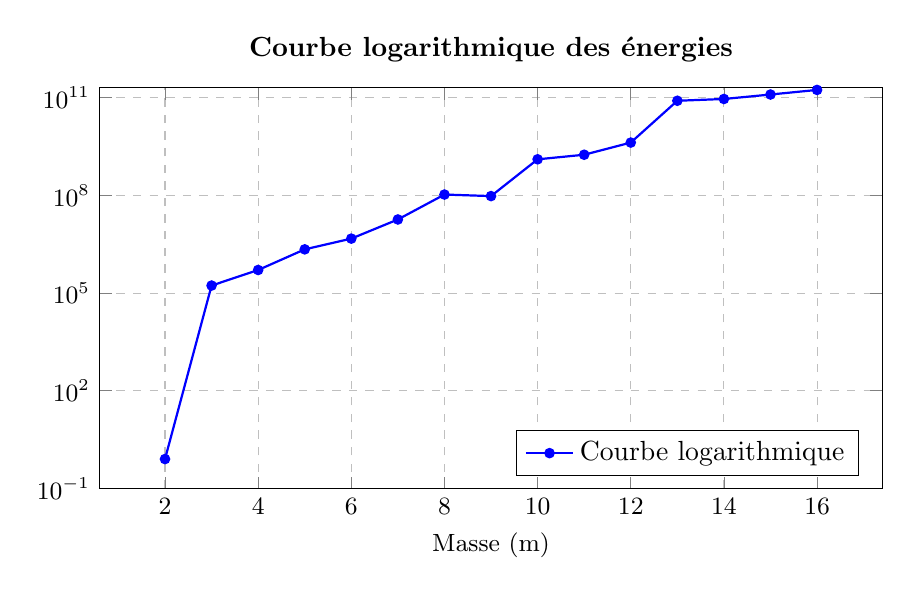
\begin{tikzpicture}
	\begin{axis}[
		width=0.95\columnwidth,          % <-- largeur exacte de la page
		height=0.55\columnwidth,     % hauteur proportionnelle (tu peux ajuster)
		%width=14cm,
		%height=9cm,
		xlabel={Masse (m)},
		ylabel={},
		title={Courbe logarithmique des énergies},
		xmajorgrids=true,
		ymajorgrids=true,
		grid style=dashed,
		ymode=log,                  % <--- échelle logarithmique sur l'axe y
		log basis y=10,
		ymin=0.1,                   % pour éviter le log(0)
		ymax=2e11,
		xlabel style={font=\small},
		ylabel style={font=\small},
		title style={font=\bfseries},
		tick label style={font=\small},
		legend pos=south east,
		]
		
		% Données (x = indice, y = valeur)
		\addplot[
		color=blue,
		thick,
		mark=*, 
		mark size=1.5pt,
		] coordinates {
			(0,0)
			(1,0)
			(2,0.8)
			(3,1.70E5)
			(4,5.11E5)
			(5,2.20E6)
			(6,4.70E6)
			(7,1.82E7)
			(8,1.06E8)
			(9,9.50E7)
			(10,1.28E9)
			(11,1.77E9)
			(12,4.18E9)
			(13,8.04E10)
			(14,9.12E10)
			(15,1.25E11)
			(16,1.73E11)
		};
		
		\legend{Courbe logarithmique}
		
	\end{axis}
\end{tikzpicture}
\end{center}
\vspace*{-0.5cm}

Les masses des particules élémentaires du modèle standard de la
physique font clairement apparaître une dispersion log-périodique. Il
existe donc un élément générateur qui suit une loi normale permettant
de reconstituer les particules élémentaires. Cet élément dépend \textit{a
	minima} d'une distance et d'un temps (structure bi-échelle) et suit une
loi fractale.

Il est raisonnable de penser que cet élément est la structure du vide. 

\begin{mybox}[breakable,colback=blue!10, colbacktitle=pkcolor]{Postulat 1}
Le vide n'est pas vide, mais est fabriqué à partir d'un élément unique.
\end{mybox}
\medskip

De façon assumée, la plénodynamique quantique part \textit{a contrario} des
idées reçues. L'éther existe et on va le construire. Einstein, qui a
démontré que l'éther luminifère, le fluide du \textsc{xix}\ieme\ siècle, n'existait
pas, n'y était d'ailleurs pas \textit{stricto sensu} opposé. À l'Université de
Leyde, le 5 mai 1920, il déclara \cite{einstein1920ether}:«En
résumé, nous pouvons dire que d’après la théorie de la relativité
générale, l’espace est doté de propriétés physiques; dans ce sens,
par conséquent, un éther existe. Selon la théorie de la relativité
générale, un espace sans éther est inconcevable, car dans un tel
espace, non seulement il n’y aurait aucune propagation de la lumière,
mais aucune possibilité d’existence pour des règles et des horloges,
et, par conséquent, aucune distance spatio-temporelle au sens de la
physique.» La physique moderne «sent» d'ailleurs qu'il y a bien
quelque chose, comme la mousse quantique de la gravité quantique à
boucles. Ici, on va franchir un pas de plus et construire un modèle
mécanique et thermodynamique de l'espace, en lui donnant une substance
réelle. C'est, en quelque sorte, un retour au source: l'éther n'est
pas un fluide luminifère, c'est un cristal luminifère.


\section{Le modèle du vide: le plenum}

Maintenant que l'existence d'une structure du vide est postulé, il est
capital de modéliser cette structure.

La première réflexion qui vient à l'esprit est que si le vide est
constitué d'un élément générateur, le vide n'existe pas. Tout le vide
est constitué de ces éléments.

\begin{mybox}[breakable,colback=blue!10, colbacktitle=pkcolor]{Postulat 2}
Le vide n'existe pas. Tout le vide est rempli d'éléments joints.
\end{mybox}
\medskip

Le vide n'étant plus vide, et pour éviter toute confusion, on
appellera désormais ce vide un plenum (du latin: assemblée pleine).
Une conséquence immédiate est que, puisque l'élément trouvé est
générateur, il est premier. Il n'existe pas d'élément plus petit. Il
ne peut donc être écrasé. L'élément est rigide.

\begin{mybox}[breakable,colback=blue!10, colbacktitle=pkcolor]{Postulat 3}
Le plenum est rigide.
\end{mybox}
\medskip

Techniquement, le plenum ressemble donc à un cristal. Il a une maille
--~l'élément générateur~-- et une rigidité.

Le plenum est donc topologiquement quantifié.

\section{Le modèle de l'élément générateur du plenum: le vorespace}
	
Il est temps de s'occuper de l'élément générateur, afin de
le modéliser.

Techniquement, toujours selon Poincaré, n'importe quel objet à deux dimensions
d'échelle, une d'espace et une de temps, devrait pouvoir convenir. On
pourra toujours extrapoler une loi plus ou moins compliquée
pour coller au modèle (qui, \textit{in fine}, doit engendrer une particule du
modèle standard). La continuité du plenum élimine cependant tout objet
qui ne soit pas capable de le remplir pleinement, par répétions, comme
un objet circulaire ou sphérique.

C'est ici que le principe du rasoir d'Ockham va servir. L'idée est de trouver
l'objet \textbf{réel} le plus simple, qui construit la loi la plus simple et
qui mène à la création des particules élémentaires.

Après quelques tâtonnements qui ont conduit à des impasses de
sur-complexité de loi\footnote{La difficulté principale est de rendre
la propriété de spin si elle n'est pas intrinsèque.}, le plus simple a
été de postuler l'existence d'un objet qui possède déjà certaines
propriétés des particules élémentaires.

On cherche donc un objet \textbf{réel} ayant au moins intrinsèquement la
propriété de spin et de charge électrique. Cet objet existe: le plus
simple est le bi-vecteur de Clifford de dimension 3, auquel on ajoute
une vitesse de rotation permettant d'assurer la chiralité, et donc la
charge électrique. La vitesse nous apporte en plus, mécaniquement,
l'unité de temps de la loi fractale.

On pourrait donc se précipiter sur cet objet, nommé $S_3$ dans l'algèbre
de Clifford, et construire notre plenum avec ce bi-vecteur. Toutefois, il serait
dommage de ne pas profiter d'une propriété de cette algèbre
géométrique. Elle postule en effet l'existence de 7 nœuds stables, des
v-sphères, nommées $S_1$ à $S_7$, chacune se construisant sur la
combinaison du nœud précédent. C'est intrinsèquement une loi
fractale. 

Le fait donc que $S_3$ soit l'objet le plus simple répondant à
notre problématique et qu'il suive déjà une loi fractale d'ordre 7 nous
pousse, toujours à cause du principe du rasoir d'Ockham, à choisir aussi cette loi
fractale comme candidate à la loi recherchée. Il se trouve que
l'algèbre de Clifford de dimension 7 reste une algèbre de Clifford,
même si on la contraint dimensionnellement, ce qui est compatible avec
notre contrainte de départ.

\begin{mybox}[breakable,colback=blue!10, colbacktitle=pkcolor]{Postulat 4}
L'élément générateur du plenum est un bi-vecteur de Clifford de
dimension 3, doté d'une vitesse de rotation et contraint
dimensionnellement. Il suit la loi fractale de l'algèbre de
Clifford de dimension 7.
\end{mybox}
\medskip

Pour faire de la mécanique avec cet objet, il est nécessaire de bien
comprendre ce qu'il est, comment il peut être représenté et comment il
fonctionne.

Techniquement, l'objet de base est composé de deux vecteurs ayant de
grandes libertés de mouvement, sept en tout. Il est très particulier
au sens où il est auto-contraint. Changer une dimension d'une partie
de l'objet (au sens d'une capacité engendrée par un des sept degrés de liberté)
change la forme globale de l'objet. Techniquement, cet objet a un module de Poisson valant $-1$, donc un module d'élasticité nul et un module de torsion infini. Il est infiniment déformable à rayon constant, mais non pliable.

Globalement, l'objet $S_3$ est une double-hélice intriquée qui forme une
turbine. La turbine possède 128 états de configuration qui lui
permettent de passer de l'état de turbine poussant dans un sens à
l'état de turbine poussant dans l'autre. Enfin, la turbine a sept
pas de vis. La contrainte de l'objet fait qu'il reste toujours une
turbine au cours de son évolution dans les 128 états possibles. On
peut voir les deux hélices emmêlées comme deux objets indépendants
seulement dans les états extrêmes des turbines. Chaque état
correspond à une mobilisation des 7 degrés de libertés possibles.
\end{multicols}

\vspace*{-1cm}
\begin{center}
	\begin{longtblr}[
		%theme=widecaption 
		caption={\footnotesize{\textbf{Description du vorespace}}},
		%label = {tblr:4-2},
		]{
			colspec={Q[2cm,c,m] Q[c,m] Q[c,m] Q[2cm,c,m] Q[2cm,c,m] Q[3cm,c,m] Q[3cm,c,m]},
			rowspec={Q[m]},
			row{odd}={bg=blue!10!white},
			row{1}={c,mode=text,fg=white,bg=pkcolor, cmd=\textbf}, %cmd=\textbf, blue!80!orange
			rowsep=2pt, colsep=3pt,
			vline{2-Y} = {1}{0.3pt,gray!50},
			vline{2-Y} = {2-Z}{0.3pt,gray!30},
			hline{Z} = {0.1pt,blue},
			% nombre de col début et fin qui apparaissent à chaque page
			% 1 pour le titre par exempel
			rowhead = 1, %rowfoot = 1, 
		}
		Degrés de liberté       &   Objet   & États  & Nombre d'états & Sens de rotation & Forme & Hélice    \\
	    3                       &    turbine aspirante  &    1 à 19  &     20   &       chiral &              cône vissé (sept pas)  &        une seule hélice tourne \\
	    4 à 7            &         idem        &         20 à 61   &   42     &     chiral     &           aplatissement         &         deux \\
	    idem     &                blocage       &        61 à 65    &   4      &      nul         &         disque obstruant    &           aucune \\
	    idem        &            turbine soufflante   &  66 à 107  &   42   &      anti-chiral &          étirement    &                  deux \\
	    3                  &        idem        &        108 à 127  &  20       &   anti-chiral     &     cône vissé inversé (sept pas) & une seule (mais l'autre) \\
	    	
	\end{longtblr}
\end{center}
%\end{multicols}

\begin{multicols}{2}

Il y a donc concrètement deux objets stables à 3 dimensions, chacun
soufflant dans une direction opposée, et de forme inversée, formant un
cône, comme une vis à 7 pas. La vis s'écrase dans un premier tas pour
former un disque qui obstrue le passage, puis croît pour former une
nouvelle vis, inversée, comme si le vissage initial traversait le
disque. Il y a clairement un effet miroir au niveau du disque de
blocage. À noter un point capital :\textit{ la transformation de l'état 1 à
l'état 128 se fait à dimension constante.}

Dans un premier temps, il n'est pas nécessaire d'approfondir davantage
les caractéristiques de cet objet extraordinaire, mais on sera
rapidement amené à y revenir. Les positions 21 à 108 vont offrir un
panel exceptionnel de possibilités pour expliquer toute la physique.
Pour construire notre plenum, on n'a besoin que d'un objet réel.
Toujours pour des raisons de simplicité, nous allons donc postuler que
l'objet réel est la turbine de dimension 3 et construire notre plenum
avec cette turbine.

On nomme $L_v$ la contrainte dimensionnelle de notre objet. Elle est donc
la plus petite distante de l'univers. Notre bi-vecteur possède de plus
une vitesse de rotation $\omega_v$. Le bi-vecteur n'étant plus tout à fait un
bi-vecteur quelconque avec ces contraintes, on l'appellera désormais
\textbf{vorespace}, par contraction de vortex et d'espace, vortex évoquant bien
l'idée de la turbine.

\begin{mybox}[breakable,colback=blue!10, colbacktitle=pkcolor]{Postulat 5}
La maille du plenum est un vorespace, un bi-vecteur de Clifford de
dimension 3, ayant une norme de dimension $L_v$, la plus petite des
dimensions, et une vitesse de rotation $\omega_v$, appliquée uniquement à
l'un des bi-vecteurs.
\end{mybox}
\medskip

Techniquement, le vorespace est une turbine à 7~pas de dimension 3.
C'est un objet tri-dimensionnel, chargé électriquement et possédant un
spin de \R{1}{2}.
\medskip

La forme étant globalement un cône, la vision cubique euclidienne de
l'élément générateur de l'espace a donc vécu$\dots$


\section{Le modèle du plenum}

Le plenum est donc un véritable champ physique, contenant en son sein
les trois propriétés fondamentales des particules élémentaires,
contrairement aux trois champs abstraits de l'électrodynamique
quantique.

C'est d'ailleurs une caractéristique de la plénodynamique quantique :
tous les champs sont des champs réels.

Pour respecter le postulat 2, on ne peut pas placer les vorespaces
n'importe comment dans l'espace. Autrement dit, le cristal est
contraint par la forme du vorespace (et réciproquement).

La première contrainte est mécanique, à cause du pas de vis. Si l'on
place deux vorespaces ayant la même chiralité à la suite, ils vont
s'opposer et se bloquer. On peut les voir comme deux roues d'engrenage
consécutives: elles tournent toujours dans des sens opposés. Le
plenum est donc composé de vorespaces à la chiralité alternative.
Physiquement, cela revient à alterner des charges positives et
négatives.

\begin{mybox}[breakable,colback=blue!10, colbacktitle=pkcolor]{Conséquence 1}
Le plenum est électriquement neutre.
\end{mybox}
\medskip

Quel que soit le volume du plenum, si l'on respecte la quantification
de maille, le volume contiendra autant de charges positives que
négatives.
\bigskip

La seconde contrainte est spatiale. Pour ne pas laisser de trou dans
le plenum, deux vorespaces voisins doivent «s'emboîter» (à la
manière d'un tore, s'entend). Si l'on prend l'image de la vis, la tête
de vis et le pied de vis doivent être tête-bêche entre deux places
voisines. Les axes de rotation de deux vorespaces sont donc retournés.
Les spins aussi. Le plenum est donc composés de vorespaces alternant
les signes de spin.

\begin{mybox}[breakable,colback=blue!10, colbacktitle=pkcolor]{Conséquence 2}
Le plenum a un spin de zéro.
\end{mybox}

\subsubsection*{Peut-on imaginer à quoi ressemble le plenum?}

Commençons à une dimension, pour que cela soit plus facile à
visualiser. Le vorespace ressemble à une vis, c'est-à-dire un cône.
Les contraintes précédentes forcent la disposition tête-bêche d'une
succession des cônes, la grande surface du premier épousant la grande
du suivant et donc la petite de la petite du suivant. On a donc une
série de doubles cônes. Visuellement, cela ressemble à une onde. Mais
comme il y a en réalité une (double) hélice qui tourne à l'intérieur,
l'image la plus parlante est celle de$\ldots$ l'ADN.

On gardera le nom, bien que les initiales désignent autre chose. Mais
l'image est belle: c'est l'ADN du plenum. On peut être physicien et
poète, cela n'est pas antinomique!

Bien entendu, le plenum est à trois dimensions, donc le brin d'ADN
doit être adapté. On peut le voir à deux dimensions comme un
empilement joint de brins d'ADN à une dimension. Chaque «contact»
s'effectue selon la même contrainte que celle de la dimension
unitaire. Les grands et les petits «diamètres» ensemble. Il est
difficile d'imaginer l'emboîtement de ces quatre surfaces, car il
s'agit d'une hypersurface. Mais concrètement, c'est l'intersection de
quatre cônes.

Bien entendu, il faut compléter la troisième direction avec un nouveau
brin perpendiculaire, pour finir de remplir le plenum. Les jonctions
deviennent difficilement visualisables.

Le modèle du plenum est terminé.
\medskip

On a bien un modèle à 3 dimensions par construction. Mais le vecteur
de Clifford sous-jacent a une structure potentielle de 7 dimensions.
Le plenum peut être vu comme un gel de 3 dimensions d'un vorespace
à 7 dimensions. Le vorespace a donc en réserve un
potentiel de 4 dimensions. On peut le voir comme «le potentiel du
vide». On le mobilisera bien entendu pour expliquer la nature des
champs électromagnétiques et de gravité.

\section{Le modèle fractal}

L'existence d'une loi fractale pour engendrer les particules
élémentaires du modèle standard est avérée par la log-périodicité des
énergies des particules élémentaires.

Essayons d'en comprendre le mécanisme. L'idée générale est la
reproduction conforme, l'auto-similarité par changement d'échelle.
On part du bi-vecteur, le vorespace, et on obtient un nouveau
bi-vecteur, à l'échelle suivante. Il faut donc prendre deux
vorespaces, chacun jouant le rôle d'un vecteur. La fusion des deux
vorespaces va donner un unique vorespace, mais de taille double. Bien
entendu, la complexité des formes va augmenter de façon exponentielle.
On a déjà du mal à imaginer correctement la turbine de base, donc une
turbine de turbine est déjà presque hors de portée de l'imagination.
L'étape suivante devient bien sûr d'une inextricable complexité. Et
comme on peut aller ainsi jusqu'à sept fois de suite, la forme de la dernière
est au-delà de tout ce qu'il est possible d'imaginer.

Par chance, en choisissant l'algèbre de Clifford comme loi fractale,
il est possible de connaître la \textit{forme combinée générale} de chacune
des étapes stables, après 7 évolutions (7 coups de vis). Les états sont donc
les nœuds de l'algèbre de Clifford, les v-sphères $S_1$ à $S_7$ et chaque
nœud aura 7 capacités de mouvement, correspondant techniquement aux fibrations. On
explicitera la forme que prendront ces nœuds dans la partie du modèle standard
de la physique.
\medskip

Quoi qu'il en soit, le mode de reproduction suit le modèle suivant:

\begin{itemize}
	\item 7 pas pour fusionner (fractalité temporelle);
	\item objet stable au 8\ieme\ pas (fractalité spatiale);
	\item l'objet stable est caractéristiquement identique au 1\ier\ objet de
	l'échelle inférieure.\footnote{Ce n'est pas tout à fait exact dans le cadre de l'algèbre de Clifford, car l'autosimilarité des différents nœuds suit aussi une loi interne que l'on mettra en évidence un peu plus loin.} 
\end{itemize}


Quand on parle de caractéristiques, il s'agit des propriétés
intrinsèques de l'objet: forme, charge (chiralité), nombre de pas de
vis (7), nombre d'états possibles (128).

Chaque objet est donc spatialement et dimensionnellement doublé par
chaque coup de vis de la fractalité, c'est-à-dire qu'un nœud stable
sera toujours une puissance $2^8$ fois plus grande que le nœud précédent.
Bien entendu, si la contrainte dimensionnelle est imposée, la taille
reste constante. On verra que cette contrainte n'est applicable que
jusqu'à la naissance du plenum et, qu'ensuite, la contrainte
dimensionnelle s'envole. Tout ceci sera explicité dans le modèle
cosmologique du Big Bang.

 \subsubsection*{Comment fusionnent deux vorespaces?}

Pour fusionner deux objets, il faut une zone de contact et un
mécanisme. Cela tombe bien, car on a construit deux vorespaces
consécutifs en contact, avec un mécanisme d'emboîtement: leur pas
de vis. Si l'un tourne, l'autre aussi.

Comment fusionner? Comme il s'agit d'une auto-réplication, les
propriétés de chacun doivent fusionner. Toute l'information de
structure de l'un doit passer à l'autre. C'est toute la beauté du
bi-vecteur: chaque tour de vis exprime le contenu complet de
l'information de sa structure. Un tour faisant $2\pi$, chaque tour
produit un contenu informationnel binaire. Au premier tour, on n'a
qu'une information, au second deux, \textit{etc.} En tout, le vorespace est
constitué de $2^7=128$ formes possibles. Chaque tour de vis entraîne de
façon mécanique un tour de vis du vorespace suivant, ce qui le
contraint à se conformer au vorespace précédent. L'information
circule. Au 7\ieme\ tour de vis, toute la structure du premier vorespace a
été transmise au second. Ils sont identiques. C'est le 8\ieme\ tour qui
provoque véritablement la fusion. Les deux vorespaces ne font alors
plus qu'un. La dimension spatiale a doublé et toutes les informations
de structure respectent ce doublement dans leur dimensionnalité (une
surface aura donc quadruplé): la dimension du nouveau vorespace est
$2L_v$, car la maille est incompressible. Seul reste constant le nombre
de tours de vis, et donc le nombre de formes possibles de la nouvelle
forme: c'est la beauté de la fractalité. On change d'échelle, pas de
forme, donc de propriétés structurelles. La progression étant
exponentielle, on se doute qu'il ne faudra que quelques dizaines de
tour pour attendre l'échelle de la particule.

Bien entendu, le mécanisme de fusion \textit{in se} n'est pas encore décrit:
il sera explicité lorsque de la description du mécanisme de la gravité.

Une conséquence triviale est que

\begin{mybox}[breakable,colback=blue!10, colbacktitle=pkcolor]{Conséquence 3}
	Toute particule élémentaire a une taille proportionnelle à une puissance de deux de la taille du
	plenum, soit $L_v$.
\end{mybox}
\medskip

Il reste à déterminer l'échelle temporelle. Elle est trivialement cachée
dans le mécanisme de vissage. C'est la vitesse de rotation qui impulse
le tempo. La réplication demande 7 tours de vis à la vitesse de
rotation du vorespace. La fusion n'est donc pas instantanée.

C'est là que les choses amusantes commencent$\ldots$ Si l'engrenage formé
par deux vorespaces n'était pas idéal, alors, par effet de bord, il
arriverait un moment où un engrenage s'arrêterait. La communication
dans le plenum serait bloquée. Pour assurer que la communication
puisse se transférer dans tout le plenum, il faut que la résistance
des engrenages soit nulle. Les turbines communiquent donc de façon
parfaite, le transfert est idéal. Par conséquence, il n'y a rien qui ne puisse 
aller plus vite. C'est le temps de transfert le plus rapide. Il est de
bon sens ici de postuler que ce temps est compatible avec c. C'est la
vitesse de propagation de l'information la plus rapide.

Le tic de l'horloge de l'univers est donc le temps de propagation de
toute l'information de structure d'un vorespace à son voisin.

On notera $\omega_v$ la vitesse de rotation du vorespace dans cette
configuration. On peut la voir de différentes manières :

\begin{itemize}
	\item soit déduite de c pour rester compatible avec la relativité
	restreinte;
	\item soit engendrant c en raison des contraintes mécaniques du
	vorespace.
\end{itemize}

En réalité, c'est la seconde qui est vraie, car la structure du plenum
qu'on a laborieusement construite avec des contraintes topologiques
pures ne sort en réalité pas du vide: elle est aussi produite
fractalement. On verra par la suite qu'il s'agit en réalité d'un
héritage de l'ère pré-planckienne, quand l'univers était purement
photonique, avant la réplication d'échelle. c\,~dépend en réalité de
la quantité d'énergie insufflée au départ du système cosmologique.
\medskip

La vitesse de rotation étant aussi une énergie, $\omega_v$ est donc 
l'énergie du vorespace. C'est l'énergie du point zéro. On peut 
la voir comme \textit{l'énergie de structure du vorespace du plenum}.
Le transfert d'information d'un vorespace à l'autre est aussi un
transfert d'énergie. Comme elle est purement mécanique (rotation de la
vis), elle est, par définition, de l'exergie. Toute l'énergie du
premier vorespace a été consacrée au transfert d'information, sans
perte. La dispergie est donc nulle, ce qui est une autre façon
d'énoncer que le système d'engrenages fonctionne sans frottement. On
retrouve l'idée de super-fluidité.

Le modèle est donc à la fois mécanique et thermodynamique. Le
mécanisme étant plus illustrant que réel, le modèle fractal est sans
aucun doute purement thermodynamique.

\begin{mybox}[breakable,colback=blue!10, colbacktitle=pkcolor]{Postulat 9}
Le plenum est géré par une thermodynamique fractale bi-échelle et
réagit comme un superfluide.
\end{mybox}
\medskip

Tout n'est donc qu'exergie dans le plenum. On peut aussi la voir d'un
point de vue informationnel. Le vorespace contient 128 états codés sur
7 v-bits. L'information n'est transférable que par unité de v-bit. Il
faut donc 7 unités de transfert pour recopier toute l'information du
vorespace. On peut donc imaginer le vorespace comme une turbine (qui
gère un flux physique) ou bien une mémoire séquentielle (qui gère un flux
informationnel). L'image des mémoires à bascules ou à registres de la
logique séquentielle est très illustrante.
\medskip

On peut ensuite se poser la question de ce que représente l'exergie de
cette onde. Si l'exergie de structure est bien illustrable au moyen d'un
engrenage, l'exergie de l'onde est plus mystérieuse.

En réalité, tout s'éclaire quand on la traduit sous la forme
informationnelle. Le vorespace est un 7 v-bit, dans lequel est codée
toute son information: chiralité, vitesse de rotation et direction du
spin. Il n'est pas nécessaire de coder le pas de vis, propriété
structurelle du vorespace. L'exergie de l'onde n'est que la transmission
de toutes ces informations au vorespace suivant.

D'un point de vue de Shannon, cette information est une entropie. Ce
qui réconcilie le point de vue «pure exergétique» au point de vue
entropique est le pas: chaque information est transférée sans perte.
La turbine est le moteur et l'entropie le flux.
\medskip

On a donc trouvé le battement de cœur du plenum. Peut-on le calculer?
\begin{equation*}
	t_v = L_v / c
\end{equation*}

Ne connaissant encore rien de la dimension du vorespace, on ne peut
rien dire de plus à ce stade.
\medskip

En conclusion, le modèle fractal du plenum est thermodynamique, basé
sur un échange d'exergie, à dispergie nulle, la maille étant le
vorespace, un bi-vecteur de Clifford de dimension 7, à norme contrainte,
avec une vitesse de rotation constante.

À noter que l'entropie du vorespace, selon Shannon, vaut 7. Le temps
de propagation de l'information est le coût entropique de Shannon, même
si le mécanisme de transfert est purement exergétique.

\section{Quelques propriétés fondamentales du vorespace}
	
Il faut dissiper très rapidement une confusion qui peut émerger de la
structure du vorespace du plenum. La rotation du vorespace lui donne
une énergie. Mais ce n'est pas une énergie mécanisable: c'est une
énergie de \textbf{structure}. Il faut la voir comme l'énergie qui permet la
rigidité (la tension) du plenum, c'est-à-dire l'équilibre du plenum.
Cette remarque topologique permet de comprendre l'erreur de calcul de
l'électrodynamique quantique quand elle trouve une valeur de $10^{120}$ à
l'énergie du vide. Elle compte l'énergie de la structure, comme une
énergie mobilisable. Ce n'est pas le cas: c'est seulement la rigidité
du cristal.

\begin{mybox}[breakable,colback=blue!10, colbacktitle=pkcolor]{Postulat 10}
Le plenum possède une énergie structurelle, non mobilisable. 
\end{mybox}
\medskip

C'est à peine un postulat, car on peut le voir comme une conséquence
de la stabilité du plenum.

On en déduit immédiatement que si le vorespace a une énergie de
structure égale à $\omega_v$, minimale, toute énergie supérieure à $\omega_v$ est
une énergie de masse.

\begin{mybox}[breakable,colback=blue!10, colbacktitle=pkcolor]{Postulat 11}
La propriété de masse découle de la différence de vitesse de rotation
d'un vorespace, d'une valeur supérieure à la valeur de stabilité
$\omega_v$.
\end{mybox}
\medskip

En conséquence, la masse est une perturbation locale de l'état
d'équilibre du plenum. On développera ce point crucial dans le modèle
de la gravité, nécessaire pour créer une dynamique dans le plenum.

\subsection{Dualité onde-corpuscule}

Le modèle thermodynamique du plenum fait émerger une dualité
ontologique. D'une part, la structure, rigide, qui n'est pas sans
rappeler l'idée de corpuscule et d'autre part, le transfert
informationnel, purement ondulatoire.

La dualité onde-corpuscule de de Broglie trouve là sa racine. On
développera plus profondément cette idée quand on détaillera la masse et la compatibilité avec la \MQ.

\subsection{L'auto-réplication, comme modèle du mouvement}

La thermodynamique du plenum redéfinit l'intuition du déplacement
physique. Il ne s'agit plus d'un objet massif --~même si l'on ne peut
pas encore parler d'objet à ce stade, mais faisons-le par anticipation~--
 qui se déplace physiquement, mais le contenu informationnel de
chaque vorespace de l'objet qui se réplique sur chaque vorespace de la
trajectoire de l'objet.

\begin{mybox}[breakable,colback=blue!10, colbacktitle=pkcolor]{Postulat 12}
Tout objet est donc techniquement un \textit{soliton topologique}.
\end{mybox}
\medskip

On note au passage que cela entraîne \textit{de facto} l'impossibilité de
téléporter un objet réel sans que cela ne viole la relativité restreinte. Il
faudrait transférer l'information de chaque vorespace plus vite que
l'information ne circule déjà, et elle circule à la vitesse de la
lumière.

Un pan entier de la littérature de science-fiction vient de
s'écrouler...

Tant que l'on n'aura pas définit proprement les objets, on ne développera pas
davantage la façon dont ils se déplacent concrètement.

\subsection{La masse comme frein à l'entropie informationnelle}

Il découle du modèle thermodynamique du plenum que si le vorespace
possède une masse ($w > w_v$), alors l'exergie de l'onde --~que l'on
appellera désormais \textit{exergie de phase} ou \textit{exergie informationnelle}~-- ne
peut plus se transmettre intégralement. Le surplus de masse agit comme
un frein pour l'onde. Non seulement la vitesse de transfert ralentit,
mais il peut aussi se bloquer si la masse est suffisante. Il existe
donc une vitesse maximale de rotation $\omega_{max}$ qui bloque le transfert
informationnel. On développera amplement cet aspect dans la partie sur
la masse.

Sans trop anticiper sur la compatibilité avec les autres physiques, on
peut d'ores et déjà avancer que le temps de propagation diminue avec
l'augmentation de la masse. C'est la contraposée d'une des lois de la
relativité générale qui stipule que la masse augmente quand le temps
diminue.

Une autre façon de voir les choses est de considérer que l'exergie
partage sa bande passante (fixe) entre l'énergie de rotation et de
translation. Plus la part dédiée à la rotation augmente, plus la part
dédiée à la translation diminue...

On développera plus largement les raisons du blocage du flux
informationnel dans la partie dédiée à la masse et à la gravité.

\subsection{La plénodynamique quantique}

La \textbf{plénodynamique quantique} se veut donc être la thermodynamique du
plenum. Elle est doublement quantifiée, spatialement par la structure
de maille du cristal du vorespace, et temporellement par la
bande-passante exergique de phase.

Il faut maintenant montrer sa capacité à engendrer les particules
élémentaires du modèle standard, en restant compatible avec les
différentes physiques.

\section{La masse et la charge électrique}

\subsection{Introduction}

Avant de passer à la reconsitution du modèle standard, il est nécessaire de bien
comprendre ce qu'est une masse et une charge électrique. Il faudra
ensuite en tirer les conséquences, à savoir la nature de la force de
gravité et de la force électrique. Et enfin, il sera
possible d'entreprendre la construction des particules élémentaires du
modèle standard.

\subsection{La masse}

La masse est définie comme un surplus de vitesse à partir de la
vitesse du vorespace. Techniquement, à cause des contraintes
inter-hélices, ce surplus de vitesse ne permet pas à la turbine de
rester dans sa zone nominale de fonctionnement, c'est-à-dire dans les positions 1 à
20. Elle doit donc aller chercher dans les positions suivantes. Le
flux décroît donc mécaniquement dans la turbine, ce qui explique le
ralentissement du temps.

La masse ne peut donc prendre que 44 positions, entre la position 21
et 64. Si la masse allait plus loin, la rotation commencerait à
s'inverser, et la masse ne serait plus une masse (techniquement, ce
serait une anti-masse, donc de l'anti-matière). À la position 64, la
masse est à son maximum: elle coupe tout le flux de transmission. Sa
vitesse est donc maximale et on l'appellera $\omega_m$.

Une masse peut donc en théorie prendre tous les états entre la
position 21 ($\omega_v + dw$) à la position 63 ($\omega_m$), soit \textbf{42 états discrets
différents}.
\medskip

D'autre part, la masse ne peut pas prendre tous ces états discrets,
car la contrainte de fusion des pales des hélices fait qu'elles
fonctionnent avec une double contrainte systémique: chaque pale a
deux contraintes d'inclinaison et deux contraintes de forme
(épaisseur et surface de la pale (longueur et largeur)). La
contrainte de fusion exige donc que chaque saut se fasse par paire de
contraintes systémiques, car changer de forme implique de changer
l'inclinaison (et vice-versa). La masse influence seulement la forme 
--~et la physique engendrée par la masse se focalisera donc sur cet
aspect. La vitesse de la masse étant une caractéristique externe aux caractéristiques du
plenum, la physique de la masse devra donc être aussi externe à celle
du plenum, dont on a vu qu'elle était purement thermodynamique. La
masse influence donc la forme de la pale pour influencer le flux du
plenum: sa physique sera une \textit{physique du flux}. Elle sera développée
dans la partie sur la gravité.

La masse ne peut donc exploiter que 44 états par paire de deux états.
Deux états finaux sont connus: ce sont les états de blocage complet
du flux. La turbine ressemble alors à un disque. La masse ne peut donc
varier que dans les 42 états précédents, soit 21 paires. Il n'y a pas
de raison que la loi de progression fractale par paliers de 7 ne
s'applique pas non plus à la masse: \textit{elle varie donc selon 7 paliers de 3
paires.}

L'apparition de la de masse s'effectue par un pas de 7 dans les 42 états
suivant les 20 premiers états d'équilibre. On peut calculer la masse
maximale possible du vorespace en gardant l'idée que $\omega_v$ est l'état
d'équilibre. On a donc à distribuer 7 flux correspondant à une partie
qui doit rester toujours à l'équilibre, c'est-à-dire $\omega_v$, soit \R{1}{7}\ieme\ de
$\omega_v$ à chaque fois. En 7 coups, on a donc impulsé 7 fois \R{1}{7}$\omega_v$, soit
$\omega_v$. La vitesse maximale est donc de $2\omega_v$.

On a donc {\boldmath{ $\omega_m = 2 \omega_v$}} 
\vfill
\clearpage

\begin{figure}[H]
	%\captionsetup{width=5cm}
	\centering
	
\includegraphics[width=0.9\columnwidth]{masse.pdf}
	\caption{\footnotesize{\textbf{Répartition de la masse dans un vorespace.} Le vorespace peut être vu, selon la masse, comme composé de 3 parties: 1 de 20 états correspondant à l'état d'équilibre (première case blanche), suivi de 21 cases représentant chaque paire gravité-charge et enfin l'état de blocage, en vert foncé. La fractalité exige que la répartition se fasse en 7 sauts, donc par saut de 3 doubles paires (en vert clair)}}
\end{figure}

À noter que ce modèle de distribution de masse est très hamiltonien.
Si $\omega$ est l'énergie du système, ce qui est le cas, alors les 128 états
possibles de la masse représentent l'espace de phase de sa distribution.
C'est un espace de Hilbert de dimension 7 ($2⁷=128$) et les $\omega$ sont les
états propres du système.

Cependant, avoir autant de masses pose un problème de simplicité
dans notre modèle de la plénodynamique quantique. Toujours en raison
du principe du rasoir d'Ockham, on stipulera qu'il n'y a qu'un seul type de masse
pour construire le modèle standard de la physique et on choisira la
plus lourde, $\omega_m$. On justifiera cette hypothèse dans le modèle
cosmologique du Big Bang.

On développera les conséquences d'un tel modèle de masse dans la
partie sur la gravité.

\subsection{La charge électrique}

Autant la masse est une aberration topologique du plenum, et donc de sa
physique, autant la charge électrique fait partie de sa nature. Il
est donc logique de gérer cette charge avec la seule physique du
plenum.

On définit la charge électrique $q_v$ du vorespace comme l'état stable de la
turbine, soit l'état des positions 1 à 20. En quelque sorte, la charge
électrique est son flux maximum (ou son flux nominal). Le flux
diminuant jusqu'à l'état 64, la charge diminue aussi. Elle s'annule au
«centre», puis s'inverse. Le signe change et la charge croit
négativement (ou positivement, si l'on part d'une charge négative).
Elle atteindra sa charge complète $-q_v$ dans les états 108 à 128.

Contrairement au cas de la masse, le cas de la charge électrique n'est
donc pas bloqué au moment de l'annulation de la charge. La physique du
plenum n'interdit en rien à la charge d'exploiter toutes les capacités
du vorespace.
\vspace*{-0.5cm}
\begin{center}
	\begin{longtblr}[
		%theme=widecaption 
		caption={\footnotesize{\textbf{Charge du vorespace}}},
		%label = {tblr:4-2},
		]{
			colspec={Q[c,m] Q[1.5cm,c,m] Q[, c,m] Q[2cm,c,m] Q[1.9cm,c,m]},
			rowspec={Q[m]},
			row{odd}={bg=blue!10!white},
			row{1}={c,mode=text,fg=white,bg=pkcolor, cmd=\textbf}, %cmd=\textbf, blue!80!orange
			rowsep=2pt, colsep=3pt,
			vline{2-Y} = {1}{0.3pt,gray!50},
			vline{2-Y} = {2-Z}{0.3pt,gray!30},
			hline{Z} = {0.1pt,blue},
			% nombre de col début et fin qui apparaissent à chaque page
			% 1 pour le titre par exempel
			rowhead = 1, %rowfoot = 1, 
		}
		États   & Nombre d'états &  Charge  &  Évolution de la charge &  Sens de rotation     \\
		1-19    &   20       &  $+q_v$  &       stationnaire      &      chiral           \\
		20-61   &   42       &  $+q_v$  &       baisse            &      chiral           \\
		62-65   &    4       &    0     &     stationnaire        &       aucun           \\
		66-107  &   42       &  $-q_v$  &       augmente          &      anti-chiral      \\
		108-127 &   20       &  $-q_v$  &       stationnaire      &      anti-chiral      \\

	\end{longtblr}
\end{center}



Comme toute la physique du plenum est gérée par une loi fractale à 7 pas, la charge
électrique n'échappe pas à la règle. Les nœuds stables étant les
charges stationnaires, il faut diviser la progression sur les 90 états
intermédiaires. D'autre part, pour les mêmes raisons qu'évoquées dans
le cas de la masse, ces états vont par paire. Mais cette fois-ci, la
physique de la charge concerne uniquement l'inclinaison de la pale.
Comme incliner la pale conduit aussi à adapter sa forme, et donc la
variation de charge, la variation d'inclinaison va de pair avec la
modification de la forme des pales. La double paire 62-65 étant
stationnaire, donc un état stable, elle ne compte pas dans les
états de transition. On a donc 84 états de transition, soit 42 paires
possibles. Avec une fractalité de 7, \textit{la charge varie par groupe de 6
paires.}

Il y a deux conséquences immédiates. La première est que la charge
varie par tiers. Elle passe de $q_v$, à \Ru{+}{2}{3}{e} et à \Ru{+}{1}{3}{e} avant de
s'annuler, puis de reprendre une progression inverse. Enfin, la
progression de la «variété électrique» est deux fois plus rapide que
celle de la masse. Voilà un début d'explication de la domination de la
force électrique sur la force de gravité.

On va désormais pouvoir étudier ces forces plus en détail.


\subsection{Les forces électriques et de gravité}

\subsubsection{Introduction}

Le modèle du plenum fabriqué précédemment souffre d'un grave défaut.
Il est statique. Comment construire les particules élémentaires du
modèle standard sans dynamique? C'est impossible! Il faut donc
trouver un moyen de créer cette dynamique. Nous allons établir qu'elle
vient (en partie) des forces électriques et de gravité. À cette fin,
nous allons nous pencher sur ces forces, même si, on le
verra, il sera nécessaire de postuler l'existence d'une particule
chargée pour terminer la démonstration des forces électriques. La
dynamique, responsable de la naissance des particules élémentaires du
modèle standard, va donc s'initier grâce à la gravité, puis se
consolider par l'effet cumulé de l'électrodynamique. C'est un modèle
très cosmologique, mais la plénodynamique quantique ne
prétend pas réinventer la physique! On verra toutefois dans le modèle
cosmologique du Big Bang que les masses possèdent aussi une vitesse de
dispersion énergétique initiale, à cause de la détente du «trou
noir» initial.

Bien que l'on pourrait ici s'intéresser uniquement à la gravité, comme
élément déclencheur, le fait que les forces électriques et de gravité
soient liées donne du sens à les aborder de concert. On mettra en
évidence l'existence de monopoles magnétiques et leur rôle dans la
gravité, en raccordant les visions de Paul Dirac et de Georges Lochak.
On établira aussi que le potentiel vecteur de l'électromagnétisme est
un véritable champ physique et, surtout, qu'il y en deux: les phonons de
gravité et ceux de charge. À partir de là, la plénodynamique quantique fera
sa première prédiction: la charge ralentit le temps, comme la masse
le fait aussi. On en déduira enfin une explication des effets
Aharonov-Bohm et Aharonov-Casher, qui seront les deux premières
preuves expérimentales de la véracité du modèle de la plénodynamique
quantique.

\subsubsection{La force électrique}

Le mécanisme de base de la force électrique est assez simple. Le
vorespace est chiral et possède un pas de vis. L'interaction entre
deux vorespaces voisins se fait structurellement via ce pas de vis. La
vision simpliste est celle d'un engrenage : si l'un tourne dans un
sens (chiral), le suivant tourne obligatoirement dans l'autre
(anti-chiral).

C'est la base. Deux vorespaces de chiralité opposée sont
structurellement liés (c'est la force d'attraction de particules de
même signe), tandis que deux vorespaces de même chiralité ne peuvent
se rencontrer sans bloquer leur rotation et rompre le plenum.
\textit{La force électrique est donc consubstantielle au plenum}. Elle lui
assure non seulement sa neutralité électrique, mais aussi sa forme.
Si le plenum est statique d'un point de vue de la structure, il est
dynamique d'un point de vue de l'énergie. On peut le voir comme un
échange permanent de flux d'un vorespace à l'autre. Par analogie avec
la mécanique des fluides, le vorespace agit comme une turbine pour le
fluide de l'information. Le mouvement du fluide est un pur
vortex, un tourbillon. Pour circuler, le fluide s'appuie sur la pale 
qui, en retour, s'équilibre par effet gyroscopique. Cet effet a toutes
les caractéristiques du champ magnétique. Il est perpendiculaire à la
pale, en sens opposé de l'appui du fluide. Il respecte bien la règle
des trois doigts par rapport au mouvement du fluide. Comme il existe
dans chaque vorespace sans boucler, c'est un monopole.

Le monopole magnétique n'est donc pas \textit{stricto sensu} une particule\footnote{On modulera plus loin cette affirmation en montrant qu'il existe réellement une particule ayant la propriété de monopole magnétique},
mais le couple de rappel d'un vorespace par réaction au passage du
flux. L'existence du monopole a été prédite par Paul Dirac en 1931 \cite{dirac1931quantised}.
Dans le cas du vorespace du plenum, étant donné l'alternance des vorespaces, les monopoles magnétiques s'annulent deux à deux. En conséquence, le magnétisme du plenum est nul.
En revanche, dès que l'on sort du cas nominal du plenum, par
adjonction de masse ou en touchant aux 88 positions potentielles, il est possible de faire apparaître
un monopole non nul.

On ne peut rien extraire d'autre du modèle statique du plenum.
Pour avancer, postulons l'existence d'une particule chargée
dans le plenum en anticipant son élaboration dans le chapitre suivant.
Quoi qu'il en soit, son existence est plausible, car elle existe dans
les particules élémentaires du modèle standard de la physique.
La chiralité de la particule n'est pas neutre par rapport au plenum.
Si on concentre en un endroit compact une super-chiralité, il se
produit une rupture de continuité du plenum autour de la particule.
C'est structurellement impossible : le plenum est un cristal rigide.
Si une rupture se présente, il se crée un vide, un vrai vide, une
absence de vorespace. Le plenum doit donc s'adapter.

La charge est directement reliée à l'angle de la rotation de la vis
(en réalité, sa double inclinaison possible). À la frontière entre la
particule massive et le plenum, les vorespaces n'ont pas d'autre choix
que de se «tordre» afin de faire riper l'engrenage. Se tordre veut
dire adapter l'angle d'engrenage. Tous les vorespaces périphériques à
la particule sont concernés. Bien entendu, il est impossible
d'encaisser sur une seule rangée la rupture d'équilibre provoquée par
la particule chargée. De proche en proche, chaque rangée de vorespaces
se tord afin d'étaler l'angle de rattrapage jusqu'à l'angle nominal du
vorespace. Visuellement, au niveau des pales turbines, il se créé un
\textit{cisaillement} à partir de la particule chargée.

Ce phénomène décrit une onde stationnaire. La particule chargée agit
comme une onde stationnaire sur le plenum afin d'assurer la continuité
du plenum pour ne pas le rompre. La forme de l'onde dépend bien
entendu de la forme de la particule, mais surtout de la manière dont
elle se transmet. Le milieu étant fractal, elle ne peut se transmettre
que par pas, selon un rythme de 7 pas avant de reboucler. L'onde est donc une rosace heptagonale
ouverte, à la manière de ce que l'on peut observer sur les photos des
novas quand elles aspirent les galaxies. L'analogie n'est pas
forcément fortuite: si l'univers suit une loi fractale, il est
normal de retrouver les mêmes images à toutes les échelles$\ldots$

On a donc crée un gradient structurel portant sur l'angle des doubles
hélices. Techniquement, l'onde varie aussi au cœur du vorespace, à
cause de la double hélicité, mais d'un point de vue macroscopique,
l'affirmation du gradient reste juste. C'est une onde de cisaillement.
En physique des solides, cette onde porte le nom de phonon. Comme le
plenum est un cristal, par analogie, on appellera \textit{phonon de
charge} cette onde de compensation de tension statique de la charge électrique.

Une conséquence immédiate est que la perturbation de l'angle
(ouvert ou fermé), sans changer la valeur de la rotation du vorespace,
induit une baisse de rendement du vorespace. En effet, le vorespace
doit «puiser» dans une des 108 positions potentielles pour s'adapter. Il
n'est plus dans sa forme nominale. La durée de transfert d'exergie
doit donc augmenter.

\textbf{Le temps ralentit donc à proximité d'une charge électrique!}

Il est clair que ce phénomène ne sera pas facile à observer à notre
échelle, car l'accumulation de charges nécessaires risque d'être
perturbée par un effet de claquage$\dots$

\subsubsection*{Comment expliquer la force électrique?}

C'est un effet purement exergétique, car la force électrique concerne
la chiralité, qui est intrinsèque au plenum. La force va donc être
gérée par la physique du plenum, qui est la thermodynamique.

Chaque particule chargée crée un phonon de charge qui est une onde
stationnaire heptagonale. Quand deux particules se rapprochent, les
ondes interfèrent. Quand deux particules ont la même charge, les ondes
s'additionnent et les vorespaces augmentent leur énergie de structure
(somme des énergies de chaque phonon). Le temps de traversée augmente, car la traversée est de plus en plus coûteuse. Les particules vont
privilégier les chemins énergétiques les plus bas (le talweg), qui
sont opposés. Elles vont reculer l'une devant l'autre. \textit{A contrario},
les particules de charges différentes s'attirent en minimisant
l'énergie sur le chemin de rencontre.

\subsubsection*{Qu'est-ce que le champ électrique?}

\textit{Le champ électrique est le gradient du phonon}. C'est donc la pente de
l'onde de cisaillement (qui est continûment ascendante ou descendante
à l'échelle macroscopique, en passant par une adaptation au sein des
deux hélices de chaque vorespace).

Comme le plenum est un cristal, on peut appliquer la loi de Hooke qui
stipule que, pour un cristal en cisaillement, le coût exergétique du
transfert est proportionnel au carré de la déformation de la maille.
En mécanique classique, on trouve que l'énergie du champ est
proportionnelle à $E^2$. Dans le plenum, la correspondance est que
l'exergie consommée est proportionnelle au carré de l'amplitude de
l'onde stationnaire de torsion.

\subsubsection*{Qu'est-ce que le champ magnétique?}

Le monopole magnétique seul ne permet pas d'induire ce qu'est le champ
magnétique. L'unique solution est de trouver une forme qui permette le
bouclage du champ sur lui-même, comme il est attendu. Sa construction
sort du cadre de cette partie. Par anticipation, on peut dire qu'un
candidat existe: c'est le hopfion.

\begingroup
\enlargethispage{0.38cm}
\endgroup
\begin{figure}[H]
	%\captionsetup{width=5cm}
	\centering
	
\includegraphics[width=0.9\columnwidth]{Hopfion.png}
	\caption{\footnotesize{\textbf{Le hopfion.} C'est le premier nœud stable du plenum qui agit en tant que dipole magnétique. On verra plus loin qu'il ressemble à un nœud $S_1$ ou $S_4$. (crédit: Wikipédia)}}
	\label{figure:1-hopfion}
\end{figure}


On note que le champ $\vec B$ étant toujours perpendiculaire à la pale et
que le phonon de charge créant une «continuité de pente de pales» dans
le plenum, le champ $\vec B$ résultant est bien perpendiculaire à cette
«onde de pales», conformément à ce que décrivent les lois de
l'électromagnétisme.

\subsubsection{La force de gravité}

Contrairement à la force électrique qui nécessite pour l'étudier de postuler
l'existence d'une particule chargée, il est possible de
créer un vorespace massique (ce qui n'a rien d'évident à prouver \textit{in
se}. On peut le postuler virtuellement pour cette partie, mais il
faudra prouver son existence par la suite. Heureusement, le modèle du
Big Bang permet de créer ces particules$\dots$) Toutefois, ce n'est pas
sans conséquence. On a vu que la masse déforme la turbine et forme
un bouchon topologique. Le plenum doit assurer la continuité autour de
la masse, pour ne pas se déchirer.

De même que l'angle varie pour la charge électrique, c'est désormais
la forme de la pale qui va s'adapter pour assurer cette continuité.
Bien que le résultat soit sensiblement identique dans la forme à celui
du phonon de charge, la dynamique qui prévaut est radicalement
différente. C'est la contrainte des pales qui donne un résultat
identique, mais la dynamique repose sur la forme dans le couple
inclinaison-forme. De même, pour la charge électrique, la dynamique
porte sur l'inclinaison. À l'instar de ce qu'il se passe pour la charge
électrique, il va se créer un \textit{phonon de masse} pour assurer la
continuité du plenum en présence d'une masse.

On aurait pu postuler que la masse cède de la vitesse aux vorespaces
aux alentours pour assurer cet équilibre. Cela aurait voulu dire que la masse
crée de la masse autour d'elle, en cédant de sa propre masse. Le
phénomène n'ayant jamais été observé, il n'a pas été retenu.
La masse crée donc un phonon de masse, c'est-à-dire une onde de masse.
C'est aussi une onde stationnaire, heptagonale. Le gradient est
l'expression du champ gravitationnel.

Attention, le gradient agit à la fois sur la crête des 7 onde,
mais aussi entre les 7 crêtes d'onde, via un double gradient$\ldots$ Il se
crée donc des talwegs d'onde masse.

On a par ailleurs vu que la physique de la masse sur le plenum n'est
plus la thermodynamique, mais la physique des flux. À noter alors le lien
profond qui apparaît avec le monopole magnétique. En effet, le
monopole magnétique est l'effet gyroscopique, la contre-réaction de la
pale au passage du flux. Si cet effet est nul dans le plenum, le
phonon de masse transforme la forme de la pale pour créer justement un
frein au flux. La gravité et le monopole magnétique sont donc
intrinsèquement liés. Cette idée rejoint celle de Georges Lochak sur
la nécessité d'avoir une masse pour le monopole magnétique \cite{lochak2002monopole}. On verra
d'ailleurs dans le modèle standard qu'il est possible de créer une
particule répondant aux critères d'un monopole magnétique et
que cette particule sera un neutrino, comme le
subodorait Georges Lochak \cite{lochak2002monopole}.

Bien entendu, comme le flux autour de la masse est perturbé par le
phonon de masse, le débit d'information n'est plus optimal,
c'est-à-dire analogue à celui du vorespace du plenum. Le temps de
traversée augmente.
\medskip

\textbf{En présence d'une masse, le temps ralentit.}

\subsubsection*{Qu'est-ce que la force de gravité?}

Analysons ce qu'il se passe quand deux masses sont proches l'une de
l'autre. On est désormais dans une physique du flux. Il y a deux cas
de figure, mais qui ont des résultats analogues quant à leurs effets.
Rien n'interdit à ce stade de la réflexion l'existence d'une masse
chirale ou antichirale. Techniquement, cela revient à avoir
une masse qui visse dans le plenum (sur un plan, on formerait une
cloche, à l'image d'une boule sur un drap) ou qui dévisse (toujours
dans un plan, l'image serait une boule qui pousse sous le drap, de
façon verticale).

En vis-à-vis des deux masses, leur phonon de masse respectif
interfère. Le flux, déjà réduit, diminue encore. Il se crée un
déséquilibre de flux entre les masses et autour des
masses. En hydraulique, un gradient de flux entraîne l'objet vers le
flux le plus tranquille. C'est le talweg du flux. Chaque masse se
dirige donc l'une vers l'autre, «roulant dans le talweg». \textit{C'est la
force de gravité.}

Il faut noter ici que la gravité respecte la thermodynamique. Si le
flux diminue, l'exergie baisse. D'un point de vue énergétique pure, les deux
masses se dirigent vers un minimum d'énergie, un talweg d'énergie.
Pour faire baisser l'exergie sans changer la vitesse de rotation du
vorespace, il faut aller puiser dans les réserves des 88 positions
possibles. C'est une augmentation d'entropie. Le talweg est
littéralement une dépression de néguentropie, la ligne de plus grande
pente vers l'état le plus «probable». Louis de Broglie l'avait
illustrée par cette image de talweg: «la trajectoire naturelle suit
le talweg d'une vallée de néguentropie.» \cite{debroglie1964thermodynamique}

Il faut ici bien comprendre ce qu'il se passe quand deux masses chirales et
anti-chirales se rejoignent. Les masses sont alors en opposition de phase.
L'une tire vers le haut, l'autre vers le bas. Leur rencontre est un
retour à l'équilibre. Techniquement, il y a une rupture de symétrie.
L'entropie extraite du plenum lui est restituée et elle est de nouveau
stockée potentiellement. Le plenum est à nouveau à l'équilibre (à
condition bien sûr que les masses chirales et anti-chirales aient la
même masse, sinon la différence forme une nouvelle masse, d'entropie de la
différence d'entropie des deux précédentes masses). On verra par la
suite que, de toute façon, ce cas n'est pas très intéressant, car
c'est juste une aberration créée dans nos accélérateurs de particules.
Le cas de deux masses de même chiralité est beaucoup plus intéressant.
D'un point de vue hydrodynamique, il n'y a aucune raison que deux
masses ne se rencontrent pas. Bien entendu, elles ne peuvent pas se
superposer, car il n'est pas possible de recouvrir deux vorespaces :
la rigidité du plenum l'interdit. En revanche, la dynamique de fusion
de la loi fractale qui régit le plenum autorise (et encourage) la 
fusion de deux masses. Deux masses ne se superposent donc pas:
elles fusionnent en une masse unique, en respectant au passage
l'échelle spatiale de la fractalité.

La gravité est donc le moteur de la fusion de notre modèle fractal.
Bien entendu, on sent bien que, si la rencontre entre deux masses est
indispensable, le plenum, en raison de l'intensité des flux au moment
de la rencontre, va subir une tension considérable, tension qu'il
faudra bien transformer en quelque chose. Ce quelque chose sera le
photon et on l'étudiera comme première particule du modèle standard,
même si \textit{stricto sensu} elle en n'est plutôt qu'un déchet de parcours.

\subsubsection{ Quelques conséquences}

\paragraph{Le potentiel vecteur}~\\ 

Les phonons de masse et de charge, s'ils sont extrêmement semblables
dans leur apparence, sont radicalement différents dans leur principe
créateur. Le phonon de charge est une onde de cisaillement et le
phonon de masse est une onde de flux. De leurs gradients respectifs,
on peut extraire une grandeur physique connue, la constante de
gravitation et le champ électrique.

Comme toujours en plénodynamique quantique, ces champs sont donc de
véritables champs physiques. On peut relier évidemment le phonon de
charge au potentiel vecteur du magnétisme, issu du rotationnel du
champ magnétique. Le magnétisme postule un champ de vecteurs purement
mathématiques. Ce champ est assurément le phonon de charge. Il existe donc bien
réellement. Comme on a vu que le magnétisme et la gravité sont
intimement liés, le champ de masse est aussi un potentiel vecteur
matérialisé. Ce sont les deux facettes d'un même champ, utilisées
différemment. C'est la raison pour laquelle la plénodynamique
quantique les différencie.

De même, le potentiel quantique de David Bohm \cite{bohm1952suggested}, dans sa théorie de
l'onde-pilote de de Broglie, est directement le phonon qui guide la
particule. On développera ce point quand on établira la compatibilité
entre la plénodynamique quantique et la mécanique quantique.

\paragraph{L'effet Casimir}~\\

Une application directe et intuitive des phonons est l'effet Casimir.
En mettant deux plaques en vis-à-vis qui sont bombardées en énergie sur
leur face opposée, il se crée une force qui aspire les plaques l'une
contre l'autre.

En bombardant chaque face, on augmente la valeur d'énergie au niveau
des plaques. Pour assurer une continuité du plenum, il se crée un
phonon de masse. L'interface des phonons entre les plaques crée une
baisse de flux qui crée une dépression, et donc l'attraction des deux
plaques.

\begin{mybox}[breakable,colback=blue!10, colbacktitle=pkcolor]{La force de gravité}
	La force d'attraction est donc un effet Casimir généralisé entre deux
	masses.
\end{mybox}
\medskip


\paragraph{Les effets Aharonov-Bohm et Aharonov-Casher}~\\


Si la mécanique quantique arrive encore à expliquer l'effet Casimir en
mobilisant l'«énergie du vide», ce qui est une façon de voir la
mobilisation de la réserve entropique du plenum qu'est le phonon, elle
n'explique pas les effets Aharonov-Bohm et Aharonov-Casher.

Quand on fait passer un électron entre deux fentes, il se forme
classiquement une figure d'interférence sur un plan de projection, si
les dimensions des fentes sont de l'ordre de la longueur d'onde de
l'électron. En revanche, placer un solénoïde chargé à proximité du
passage de l'électron perturbe la figure d'interférence, faisant
apparaître un retard de phase.

Le champ magnétique $\vec B$ n'étant présent --~selon les lois de l'électromagnétisme~-- qu'à l'intérieur du solénoïde, comment un électron
«sent-il» la présence du champ, alors qu'il passe à l'extérieur du solénoïde? La
physique actuelle ne l'explique pas.

En réalité, la frontière au niveau du solénoïde ne peut être brutale
au niveau du plenum. Il se crée un phonon de charge à l'extérieur.
L'électron traverse ce phonon, qui n'est plus un plenum équilibré. Le
temps de traversée augmente. La phase se décale.

Une preuve expérimentale de l'existence ce phonon serait de reculer le solénoïde.
Il existe une distance à laquelle le phonon de charge s'équilibre avec
le plenum. L'électron ne serait alors plus déphasé. Une expérience
avec une série de distances croissantes doit mettre en évidence un
retard de phases décroissant.

De même, la physique classique n'explique pas l'effet Aharonov-Casher.
Il s'agit cette fois de faire circuler une particule ayant un moment
magnétique, comme un neutron par exemple, le long d'une ligne
chargée. Il se crée cette fois un décalage de l'angle du spin. En
l'absence de champ magnétique, ce phénomène est inexplicable. La
présence d'un phonon de charge, en raison de la ligne électrique,
explique la présence du champ perturbateur. De même, on doit pouvoir
mettre en évidence la distance de coupure du champ via un protocole
similaire au précédent.

\subsubsection{Conclusions}

La force électrique, consubstantielle au plenum, est
régie par la thermodynamique. La force de gravité, contre-naturelle
au plenum, est régie par une physique différente de la physique
d'équilibre du plenum. C'est une physique des flux. Ces deux forces
font apparaître, chacune à leur manière, une torsion du plenum pour
assurer sa continuité sans le rompre. Comme le plenum est un cristal,
ce sont deux phonons, de charge et de masse. En réalité, les deux
phonons sont liés : la torsion est le moteur de l'un et la gestion du
flux le moteur de l'autre. Ce sont les deux faces d'une même pièce,
selon la façon dont elles sont employées. Le gradient des phonons donne
alors les valeurs des champs électrique et gravitationnel. On note
que le champ gravitationnel et le champ magnétique sont liés par le
même mécanisme. Enfin, le monopole magnétique existe, comme effet
gyroscopique des pales du vorespace au passage du flux entropique. Il s'annule
à l'équilibre et se révèle bien entendu quand l'entropie
augmente.


\section{Le modèle standard de la physique}

\subsection{Introduction}

Pour le moment, le modèle proposé est satisfaisant, car il est
compatible avec l'électromagnétisme et la gravité. Il explique de
plus les effets Aharonov-Bohm et Aharonov-Casher, ce qui n'est pas
rien. Il doit désormais expliquer la création des particules
élémentaires du modèle standard pour être validé.

Il faut au préalable mettre au jour la véritable nature du photon. En effet, jusqu'à présent, la
physique ne faisait que constater l'existence du photon et en prendre
acte. Nous allons répondre à la grande question que se posait Albert
Einstein: «Si seulement on pouvait comprendre $E=h\nu$!»\cite{einstein1994correspondence} On va
découvrir que le photon est hors-modèle, car il est, à l'instar de la
force de gravité, une anomalie du plenum. Mais au lieu d'être une
anomalie utilisant du potentiel du vide, il est une anomalie de
structure, de dimension.

\subsection{Le photon}

\subsubsection{Le modèle du photon}

Le problème consiste à construire un photon à partir de vorespaces du plenum, qu'ils
soient massiques ou non. Ce sont en effet les seuls «outils» à notre
disposition et nous ne pouvons pas faire autrement que de
utiliser.

La difficulté est de créer une particule de spin 1 à partir de
particules de spin \R{1}{2}. La solution évidente est d'assembler deux
particules de spin \R{1}{2}. Dans le plenum, deux vorespaces consécutifs
sont alternés, pour assurer une neutralité électrique, mais aussi la
nullité du spin. Il faut donc retourner un vorespace pour en mettre
deux en vis-à-vis. La tête de vis de l'un fait donc face à la pointe
de vis de l'autre. La somme des spins fait bien 1: le
«double-vorespace» est un boson. L'image d'un photon composé de deux
demi-photons de Louis de Broglie prend corps. \cite{debroglie1934une}

Deux problèmes surgissent instantanément. Il est impossible de
retourner un vorespace dans le plenum sans déchirer le plenum lui-même, car il est rigide.
Techniquement, il est donc impossible de créer un photon par la loi
fractale du plenum.

Supposons toutefois que cela soit possible. Ce double-vorespace est en
réalité un couple (vorespace, anti-vorespace). Les deux vorespaces sont
en tout point identiques, mais de façon miroir. Ils doivent
s'annihiler. Quel est donc ce processus, d'où vient-il et que
produit-il au final?

La création d'un photon dans le plenum est \textit{a priori} une impossibilité
structurelle. Le photon est techniquement une aberration topologique,
et son processus d'élaboration est contraire aux lois du plenum.
Heureusement, la gravité vient sauver le photon.

Revenons à l'instant où deux masses se rapprochent pour fusionner. Leurs
phonons de masse s'additionnent, créant sur le chemin des
vorespaces hyper-entropiques. Leur vitesse est toujours $\omega_v$, mais
l'onde de cisaillement écrase littéralement la turbine en
l'aplatissant: il arrive un moment où la turbine devient un
«disque» , obstruant tout le passage. Le flux est alors coupé.
L'approche des masses étant symétrique, on est assuré qu'au moins deux
vorespaces voisins ont atteint cet état.

La pression sur les vorespaces devient gigantesque, puisque d'un côté
le flux est nul et que, de l'autre, il est très grand. Tout est
bloqué. Cependant, la masse a une vitesse qui excède la vitesse de
rotation du plenum bloqué. Elle peut donc encore forcer en cédant une
partie de son énergie excédentaire. Le coup de vis supplémentaire
vient donc à bout de la résistance du plenum, qui «craque». Pour
faire craquer le plenum, la masse doit donc céder une énergie
correspondant à la masse du vorespace, soit $\omega_v$.

Visuellement, les deux vorespaces, qui sont des disques, entrent
l'un dans l'autre. La pénétration se fait au détriment de la surface.
En 7 pas, elle s'arrache complètement. Au 8\ieme\ pas, les deux sphères
deviennent deux disques entrelacés.

Concrètement, les vorespaces ont perdu leur surface, qui venait du 3\ieme\
degré de liberté. Les deux cercles sont donc un vorespace à deux
degrés de liberté. On pourrait alors s'amuser à élaborer plein de
théories pour trouver à quoi ressemble ce nouvel assemblage, mais cela
a déjà été fait. C'est toujours un bi-vecteur de Clifford, mais à deux
degrés de dimension, une v-sphère $S_2$. Elle est composée de deux
cercles perpendiculaires qui ont une rotation liée, permise autour
d'un axe qui les relie en les «soudant» autour de deux points fixes.

La meilleure image que l'on puisse s'en faire est celle d'un cardan.

On remarque immédiatement que deux cercles en rotation liée forment un
photon. La gravité, en pliant le plenum, a donc créé un photon.

Le processus n'est pas terminé. Les masses continuent leur poussée sur
le photon qui se met en rotation. Il tourne évidement selon un
processus à 7 pas, donc par pas de $2\pi/7$. À chaque pas, les deux
cercles s'enroulent autour d'un vorespace voisin et, au septième, ils
se sont totalement enroulés. On remarque alors que le photon n'a fait
lui-même qu'un demi-tour. Rien ne freine le photon, car il n'entre pas
en interaction avec le vorespace. Il ne peut donc que continuer à
s'enrouler. À la fin du second vorespace, il finit sa propre rotation
complète. Il lui faut donc deux vorespaces pour effectuer une rotation
complète, confirmant l'intuition de de Broglie que le photon soit
composé de deux demi-photons. En réalité, sa dimensionnalité inférieure
l'oblige à s'adapter à son nouvel espace.

Rien n'arrête plus le photon qui s'enroule toujours selon les brins
d'ADN du plenum. Il circule donc à la vitesse nominale de transmission
d'un vorespace, c'est-à-dire à c.

\subsubsection{Les conséquences}

Il y a énormément d'informations dans le processus précédent. Le photon est une
rupture de symétrie du plenum qui est un équilibre thermodynamique. En
tant qu'anomalie topologique, sa co-existence dans le plenum en tant
que particule statique est impossible: le photon ne fait pas partie de
l'univers du plenum. Sa dynamique est donc une réponse à cette
impossibilité: il est condamné à fuir, ne pouvant se fixer. Sans
masse, il circule comme un superfluide, à la vitesse maximale
autorisée par le plenum. Mais sa vitesse et sa masse sont aussi un
moyen de conserver la masse statique du plenum, sans quoi la
disparition de deux vorespaces changerait l'équilibre global du plenum.
L'énergie totale est  bien conservée. Chaque masse fusionnée a perdu
l'énergie d'un vorespace, donc diminué sa rotation de $\omega_v$.\footnote{On verra en réalité que le processus est dynamique et que le coût exergique est décomptée du mouvement.} L'énergie
totale du plenum n'a pas été modifiée.

Une conséquence est que la physique du photon est aussi différente de celle du plenum, 
qui est purement exergique, à l'instar de celle de la force
électrique. La force de gravité est quant à elle une physique du flux. La physique
du photon repose ainsi uniquement sur l'entropie. Le photon est en quelque sorte \textit{un
révélateur entropique}. Par son double-mécanisme d'emboîtement, de
l'ouverture du photon et de la rotation de la vis du vorespace, le
passage du photon est littéralement «collé» au vorespace et le suit
dans toutes ses fluctuations entropiques. 

En conséquence, le photon,
non seulement décode l'entropie du vorespace, mais se dirige toujours
vers les gradients positifs du phonon, c'est-à-dire en «surfant sur
la crête entropique» ou, comme l'avait dit Louis de Broglie, «en
suivant les talwegs de néguentropie». Dit autrement, c'est le
second principe de la thermodynamique qui est mis à jour, non pas
comme un principe sorti de l'expérience humaine, mais comme une
contrainte de vissage entre un photon et un vorespace. 

\begin{mybox}[breakable,colback=blue!10, colbacktitle=pkcolor]{Second principe de la thermodynamique}
	Le second principe de la thermodynamique est en réalité un mécanisme 
	structurel.
\end{mybox}
\medskip


De plus, la création du photon permet de finir d'élaborer la fusion de
masse fractale. Il est nécessaire qu'il y ait un nombre pair de
vorespaces entre les masses. Quand le groupe de paires ou la paire de
vorespaces atteint son entropie maximale, alors la gravité peut les
transformer en photons, pour finir d'ouvrir la voie. Quand il n'y a
plus de vorespace entre eux, les masses sont en contact. \textit{C'est la
fusion}. Il est probable que l'émission de photon suivent aussi une loi
de création par groupe de 7.

Enfin, le photon, en tant que sous-produit de la gravité, révèle en
miroir une structure sous-jacente du plenum. Si l'on peut briser la
symétrie des particules, on peut briser la symétrie de la structure
entière. \textit{On pressent alors que le plenum est le résultat d'une
structure précédente à deux dimensions via un passage fractal}. Le
photon est donc une résurgence du passé. On verra par la suite, grâce
au modèle du Big Bang, qu'il est en réalité comme un jeune conducteur qui
découvre l'ivresse de la vitesse. Quoi qu'il en soit, cela
«justifie» la répartition d'énergie supposée, en divisant par deux
dans la «fusion arrière». La loi fractale doit être respectée dans
le passage à l'échelle. On reviendra sur tout cela quand on abordera
le modèle du Big Bang.

\subsection{Le modèle des particules élémentaires du modèle standard}

Attaquons-nous désormais à la construction des particules élémentaires
du modèle standard de la physique. À cette fin, on postulera une
abondance de masses élémentaires de vitesse $\omega_m$. La processus de fusion
se fera via la gravité et suivra un processus fractal non
dimensionnellement restreint.

Pour rappel, la liste des particules élémentaires à créer est rappelée dans le tableau \ref{tblr:4-epe}.

\vspace*{-0.5cm}
\begin{center}
	\begin{longtblr}[
		%theme=widecaption 
		caption={\footnotesize{\textbf{Énergie des particules élémentaires}}},
		label = {tblr:4-epe},
		]{
			colspec={Q[c, co=1]  Q[c] Q[c, co=1] },
			rowspec={Q[m]},
			row{odd}={bg=blue!10!white},
			row{1}={c,mode=text,fg=white,bg=pkcolor, cmd=\textbf}, %cmd=\textbf, blue!80!orange
			rowsep=2pt, colsep=3pt,
			vline{2-Y} = {1}{0.3pt,gray!50},
			vline{2-Y} = {2-Z}{0.3pt,gray!30},
			hline{Z} = {0.1pt,blue},
			% nombre de col début et fin qui apparaissent à chaque page
			% 1 pour le titre par exempel
			rowhead = 1, %rowfoot = 1, 
		}
		Particules               &   Désignation         & Masse                    \\
		Photon                   &        $\gamma$       &  0                       \\
		Gluon                    &            g          &  0                       \\
		Neutrino électronique    &        $\nu_e$        &  < 0,8 $eV/c^2$          \\
		Neutrino muonique        &        $\nu_\mu$      &  < 0,17 $MeV/c^2$        \\
		Électron                 &           $e^-$       &  0,511  $MeV/c^2$        \\
		Quark up (u)             &            u          &  $\approx$ 2,2 $MeV/c^2$ \\
		Quark down (d)           &            d          &  $\approx$ 4,7 $MeV/c^2$ \\
		Neutrino tauique         &        $\nu_\tau$     &  < 18,2 $MeV/c^2$        \\
		Muon                     &        $\mu^-$        &  105,7 $MeV/c^2$         \\
		Quark strange (s)        &            s          &  $\approx$ 95 $MeV/c^2$  \\
		Quark charm (c)          &            c          &  $\approx$ 1,28 $GeV/c^2$\\
		Tau                      &         $\tau$        &  1,77 $GeV/c^2$          \\
		Quark bottom (b)         &            b          &  $\approx$ 4,18 $GeV/c^2$\\
		Boson W                  &         $W^\mp$       &  80,4 $GeV/c^2$          \\
		Boson Z                  &           $Z_0$       &  91,2 $GeV/c^2$          \\
		Boson de Higgs           &           $H_0$       &  125,1 $GeV/c^2$         \\
		Quark top (t)            &            t          & $\approx$ 173 $GeV/c^2$ \\
	\end{longtblr}
\end{center}


Il va donc falloir faire entrer cette liste dans un processus fractal.
Or il a été choisi initialement le processus fractal de l'algèbre de
Clifford, à savoir 7 nœuds possibles, les $S_1$ à $S_6$. Ces
nœuds vont donc être composés de vorespaces massiques, en progression
de la loi fractale.

On peut se les représenter et obtenir quelques informations
caractéristiques (\textit{cf.} tableau \ref{tblr:5-0-1}).
On voit donc clairement apparaître une composition naturelle de $S_1$ à
$S_6$, avec trois formes (cercle, double-cercle et hélice), avec une rupture
de composition pour la 7\ieme\ forme qui est une fin dans l'algèbre de
Clifford.

Postulons donc qu'à cette échelle, la fin du processus conduise à nos
premières particules physiques, les hadrons, à savoir le neutron et le
proton. Techniquement, le neutron et le proton seraient des nœuds $S_8$.

%\vspace*{-0.5cm}
\begin{table}[H]
	\centering
	\caption{\footnotesize{\textbf{Nœuds de l'algèbre de Clifford $S_{7,0}(\mathbb{R}$)}}}
	\label{tblr:5-0-1}
	\begin{tblr}[
		%theme=widecaption 
%		caption={\footnotesize{\textbf{Nœuds de l'algèbre de Clifford $S_{7,0}(\mathbb{R})$}}},
%		label = {tblr:5-0-1},
		note{$\dagger$} = {composée de vorespaces, donc c'est une suite ressemblant au brin	d'ADN, un tube continu variant d'un maximum à un minimum.},
		]{
			colspec={Q[c,m]  Q[2cm, c,m] Q[4cm,c,m] Q[c,m] },
			rowspec={Q[c,m]},
			row{odd}={bg=blue!10!white},
			row{1}={c,mode=text,fg=white,bg=pkcolor, cmd=\textbf}, %cmd=\textbf, blue!80!orange
			rowsep=2pt, colsep=3pt,
			vline{2-Y} = {1}{0.3pt,gray!50},
			vline{2-Y} = {2-Z}{0.3pt,gray!30},
			hline{Z} = {0.1pt,blue},
			% nombre de col début et fin qui apparaissent à chaque page
			% 1 pour le titre par exempel
			rowhead = 1, %rowfoot = 1, 
		}

		Nœud    & Quantité de vorespaces   &            Forme\TblrNote{$\dagger$}                   & Spin \\
		$S_1$   &         $2^8$            &        Cercle                                          &  0   \\
		$S_2$   &         $2^{16}$         &        2 cercles perpendiculaires                      &  1   \\
		$S_3$   &         $2^{24}$         &        Double hélices entremêlées                      & \R{1}{2}  \\
		$S_4$   &         $2^{32}$         &        Tore des doubles hélices précédentes            &  1   \\
		$S_5$   &         $2^{40}$         &        2 tores précédents perpendiculaires             &  1   \\
		$S_6$   &         $2^{48}$         &        Double hélices des tores précédents             & \R{1}{2}  \\
		$S_7$   &         $2^{56}$         &        7 doubles hélices précédentes emmêlés en hélice & \R{1}{2}  \\
	\end{tblr}

\end{table}

Ils doivent donc être composés de $2^{64}$ masses élémentaires, ce qui
revient à dire que leurs tailles sont proportionnelles à la taille de la
masse élémentaire, donc du vorespace :

\begin{equation*}
	L_{hadron}  = 2^{64} \cdot L_v
\end{equation*}


On a donc $L_v = L_{hadron}/2^{64}$

avec
\begin{equation*}
	\left\{
		\begin{split}
	 		L_{neutron} &= 0,8 \cdot 10^{-15}\,m  \\ 
	 		L_{proton}  &= 0,88 \cdot 10^{-15}\,m 
		\end{split}
	\right.
\end{equation*}

$L_v$ oscille donc entre $4,3 \cdot 10^{-34}\,m$ et $4,8 \cdot 10^{-34}\,m$, soit un peu plus
de 20 fois la longueur de Planck ($L_p=1,6 \cdot 10^{-35}\,m$). Sachant que c'est
une approximation de la longueur du hadron, ce résultat conforte
l'hypothèse hadronique comme résultat de la périodicité de Bott. On
pourrait donc avoir


\begin{equation*}
	L_v \approx 20 L_p
\end{equation*}

On ajustera cette longueur grâce aux propriétés du photon, dans la
partie réservée aux constantes de la physique.
\medskip

Tâchons de voir désormais comment ranger les particules élémentaires
dans les nœuds de l'algèbre de Clifford. On a déjà un problème
évident : il y a plus de particules élémentaires que de nœuds. De
plus, un nœud étant stable, il a donc une unique énergie et on ne peut
ranger deux particules de massses différentes dans le même nœud. On a
donc au moins 17 particules à essayer de faire entrer dans 7
nœuds.

Il y a un premier tri assez facile à faire. Il suffit de comparer les
valeurs de spins. Le gluon, avec sa masse nulle, ne peut entrer nulle
part. Les bosons Z et $W^\pm$, avec leur grande masse, correspondraient à
des particules très lourdes, donc des $S_6$ ou des $S_7$. Leur spin de 1
rend cette appartenance impossible. De même, les neutrinos ont des
masses très légères, donc devraient être des nœuds $S_1$ ou $S_2$ au
maximum. Leur spin de \R{1}{2} rend aussi impossible cette appartenance.
Les quarks, avec leurs charges fractionnaires, rendent problématique
un rattachement à un quelconque nœud: nulle part, dans la loi de
fractalité, la chiralité se divise. Il ne reste donc que l'électron,
le muon et le tau. Leurs spins les obligent à être au moins un nœud
$S_3$ et leurs énergies placeraient ces particules dans les nœuds
suivants:

\begin{center}
\begin{tabular}{ c c l }
	$S_3$ & $\rightarrow$ & électron \\
	$S_6$ & $\rightarrow$ & muon     \\
	$S_7$ & $\rightarrow$ & tau 
\end{tabular}
\end{center}

Examinons rapidement le cas $S_3$ pour l'électron. $S_3$ est un passage à
l'échelle du vorespace, donc si ce cas est avéré, cela veut dire que
les positions 1 à 19 de l'électron correspondent à la charge
élémentaire de l'électron, soit $q=-1,6\cdot10^{-19}\,C$. La charge est une
caractéristique interne du vorespace, elle est invariante par
changement d'échelle. On en déduit que la charge élémentaire du
vorespace est aussi q, donc $q_v=-e$. On retrouve bien que la charge est
un invariant relativiste.

C'est tout ce qu'il est possible de déduire à ce stade. On pourrait croire
que le modèle standard n'est pas compatible avec la loi fractale de la \PQ.

Est-ce la fin de la partie? Non, car jusqu'à présent, on a supposé
que le modèle engendrait ses nœuds sans interagir avec le plenum, ce
qui est clairement faux. On a vu qu'au niveau du plenum, quand deux
charges fusionnent, il se forme au moins un photon. Se pourrait-il
qu'il se produise d'autres particules?

Examinons les cas et appliquons résolument la loi fractale à partir de
la masse unitaire.

\subsubsection{Premier nœud: la première particule de l'univers}

Le premier nœud $S_1$ rassemble donc $2^8$ vorespaces massiques. Chaque
paire a engendré (au moins) un photon et, par conséquent, chaque
liaison s'est trouvée réduite de la masse d'un vorespace du plenum. Le
nœud forme un cercle de 256 vorespaces. C'est un élément extrêmement
léger qui aurait pu faire un candidat au rôle de neutrino, si son spin
de 0 avait été compatible.

Malheureusement, dans la description précédente de la fusion de deux
vorespaces massiques, il n'a pas été tenu compte de leur vitesse de
rotation. Quand deux vorespaces massiques s'associent, ils ne peuvent
s'associer que tête-bêche, les parties hautes des turbines ensemble.
Cette association implique que les turbines tournent en sens
contraire. Si l'on associe deux turbines chirales, il faut trouver un
processus qui inverse la chiralité de l'une pendant le processus de
fusion. Cette opération est forcément asymétrique (l'une change de
chiralité, pendant que l'autre reste chirale) et exige un processus
compliqué. Il est bien plus simple, toujours selon le principe du rasoir d'Ockham,
de postuler l'existence d'un vorespace massif anti-chiral. Cette
hypothèse sera confirmé lors du modèle du Big Bang.

Dès lors, le processus évoqué précédemment reste pertinent, et même
favorisé, puisque deux vorespaces massifs anti-chiraux vont se
rapprocher plus facilement, comme lors d'une rencontre de deux
particules de charge opposée. Quoi qu'il en soit, on verra que dans le
modèle du Big Bang, les particules ont en plus une cinétique très
importante, qui prendra de toute façon le pas sur tout.
Les vorespaces du plenum subissent donc exactement le même processus,
à la différence près que deux vorespaces voisins se mettent chacun
dans l'état de disque, soit par un processus décroissant (44\ieme\
paire, position 62-63), soit par un processus croissant (66\ieme\ paire,
position 63-64). Techniquement, leur position respective, l'un placé «au-dessus» de
l'autre, favorise la rencontre, puis le déchirement et la perte
dimensionnelle qui s'ensuit. Le photon naît donc de la fusion d'un
vorespace massif et d'un vorespace anti-massif.

L'élément obtenu garde la chiralité du vorespace massif. S'il y autant
de vorespaces massifs qu'anti-massifs (hypothèse qui sera justifiée dans
le modèle du Big Bang), il se crée autant d'éléments chiraux
qu'anti-chiraux et le processus peut se répéter. À la 7\ieme\ étape, il
n'existe plus que deux types d'éléments : un élément chiral de 128
vorespaces et un élément anti-chiral de 128 éléments. Le nœud suivant
est celui de la stablitié, ce qui veut dire implicitement que tous les
éléments massifs (et donc anti-massifs) ont été consommés.
La première particule massive est donc un nœud $S_1$. Elle ressemble à
un tore d'ADN chiral, composé de 256\,~masses élémentaires, et donc de
périmètre $256 \cdot 2L_v$, soit $512 \cdot 1,616 \cdot 10^{-35} = 8,274 \cdot 10^{-33}\,m$. Son rayon
est donc $5,267 \cdot 10^{-33}\,m$.

On peut essayer d'imaginer le phonon de masse engendré par une telle
particule. La rotation du tore, par pas de $2\pi/7$, engendre une onde
heptagonale. La rotation interne des doubles-hélices ajoute une onde
heptagonale dans le sens des pales qui va favoriser le chevauchement
de deux particules de ce type.

\subsubsection{Nœud $S_2$: la seconde particule de l'univers}

En effet, l'étape suivante consiste à créer un nœud $S_2$ à partir de
deux nœuds $S_1$. On est toujours dans un processus forcé dynamiquement,
mais dès ce stade, la gravité peut suffire à expliquer complètement le
processus. Deux nœuds $S_2$ se rapprochent par gravitation pure. À cause
des phonons «perpendiculaires», ils ne peuvent fusionner dans le
plan de rapprochement, comme à l'étape 1. Les deux phonons les
obligent à se chevaucher, donc à passer l'un sur l'autre. Les deux
phonons «perpendiculaires» les placent donc là où le flux est 
moindre, c'est-à-dire perpendiculairement l'un à l'autre. La pression fait le
reste et les deux tores s'emboîtent en 7 fois $2\pi/7$\ieme\ de tour de tore
respectif. La chiralité est identique sur les deux tores et est donc
conservée à l'ensemble: le «primo-photon» de masse $S_2$ est né. À
noter qu'à l'interface des jonctions, les vorespaces du plenum sont
écrasés selon un processus identique à celui de l'étape 1: il se crée donc
encore des photons.

Bien entendu, le processus continue par fractalité. 2
«primo-photons» fusionnent, chaque tore perpendiculaire fusionnant
 selon un processus de double-enroulement. Le processus se
répète 7 fois, produisant son lot de véritables photons, jusqu'à
l'étape final du nœud $S_2$, à la huitième étape.

La seconde particule de l'univers ressemble donc à deux tores
(eux-mêmes composés de 7 tores enroulés) d'ADN imbriqués,
perpendiculaires l'un à l'autre, en rotation chirale, chaque tore
faisant un $2\pi/7$\ieme\ de tour à chaque fois. Il est composé de $2^{16}$
éléments de masse élémentaire. Le phonon de masse commence à être
difficile à décrire. Il s'agit en réalité d'un sous-ensemble de la
fibration de Hopf qui ne garde que 7 cercles de la fibration, chacun
étant bien entendu décalé de $2\pi/7$. Malgré tout, on ne peut imaginer
réellement qu'un seul phonon à la fois à chaque étape de la fibration, car imaginer leur
combinaison commence à faire mal à la tête$\ldots$ Quoi qu'il en soit, on
commence à se rapprocher d'un champ gravitationnel sphérique autour de
la particule, même s'il est $2\pi/7$-périodique.

\subsubsection{Le troisième nœud: et l'électron fut}

Il faut répéter ce processus pour le troisième nœud, avec un
processus fractal qui va aussi se développer dans la troisième
dimension, ce qui nous mènera mécaniquement à $2^{24}$ masses élémentaires
pour sa composition. L'idée générale sera de «dévisser» chaque tore,
en l'élevant dans une dimension verticale. Le dévissage se fera de
concert avec les deux tores perpendiculaires, entraînant un
emboîtement des déroulements, et donc, au final, une double-hélice. La
dimension grossissant aussi par pas de $2\pi/7$, la largeur de
l'enroulement sera plus grande à l'arrivée qu'au départ, d'où la forme
de turbine. Enfin, la rotation ne pourra être transmise qu'à l'une
des deux hélices, sinon le processus de déroulement ne serait pas
possible: en quelque sorte, l'une cède peu à peu sa rotation pour
permettre la rotation de l'ensemble dans la dimension supérieure.

On peut quand même essayer de décrire le processus de fusion. Deux
particules $S_2$ fusionnent. Il n'y plus de possibilité d'enrouler les
tores avec les 7 déjà enroulés, donc le tore est obligé de rester
extérieur à l'enroulement. Le processus se faisant par pas de $2\pi/7$,
il se crée un décalage spatial et angulaire de $2\pi/7$ entre les deux
tores. Il en va de même avec le tore perpendiculaire. L'équilibre de
rotation de l'ensemble est perturbé et pour que les deux $S_2$ restent
emboîtés, le tore perpendiculaire doit céder $2\pi/7$ de sa vitesse
angulaire. Le processus se répète 7 fois, jusqu'au premier nœud
primo-stable. Il s'est crée deux pas de vis emmêlés qui est le premier
pas de vis de la particule finale. Ces primo-nœuds rencontrent
d'autres primo-nœuds en fusionnant pour donner, à chaque fois, un pas
de plus, jusqu'au 7\ieme\ nœud, c'est-à-dire le nœud $S_3$.

On se retrouve à cette étape avec une copie conforme du vorespace massique, à
l'échelle, composée de $2^{24}$~éléments massiques. Sa
structure compatible avec la définition d'une charge électrique et son
spin de \R{1}{2} le rend compatible avec le rôle de l'électron. Sa masse
totale inclut toutes les énergies de fusion, parties en photon.

Si l'on accepte que le nœud $S_3$ est bien un électron, alors:

\begin{itemize}
	\item l'électron serait la première particule élémentaire connue de l'univers
	créée dans ce processus;
	\item le vorespace a bien une charge de $e=1,6 \cdot 10^{-19}\,C$.
\end{itemize}

On peut calculer la masse élémentaire fusionnée :
\begin{equation*}
m_{e^-_{fusion}} = \frac {0.511 \cdot 10^6} {2^{24}} = 3,05 \cdot 10^{-2}\,eV/c²
\end{equation*}

Bien entendu, il faut retirer les énergies de chaque
photon engendrées par la fusion, et donc connaître l'énergie de masse du
vorespace. Or on sait que $\omega_m = 2 w_v$ et que chaque vorespace a coûté
une fusion, donc on en déduit que
\begin{equation*}
m_{e^-} = \frac{1}{2} m_{e^-_{fusion}} = 1,52 \cdot 10^{-2}\,eV/c²
\end{equation*}

et, de fait, $m_{v_{massique}} = 0,75 \cdot 10^{-2}\,eV/c²$
\medskip

À noter que le champ gravitationnel devient extrêmement complexe. Il
s'agit encore d'une fibration à 7\,~pas, mais la triple imbrication des
rotations rend la visualisation du champ résultant extrêmement
difficile à concevoir.

\subsubsection{Le nœud 4 ou le combat des forces}

\paragraph{Le modèle de concurrence charge-gravité (CCG)}~\\

Jusqu'ici, la fusion est purement gravitationnelle. Mais à partir de
$S_3$, le nœud comporte une charge et il va falloir en tenir compte.
En effet, le nœud suivant, selon la logique de la loi fractale, doit
faire fusionner deux $S_3$, soit deux électrons ensemble, leur charge de même signe
rendant théoriquement le rapprochement impossible. Il est nécessaire
d'introduire une énergie permettant d'outrepasser cette
impossibilité. On admet pour la suite que les électrons sont dotés
d'une vitesse, et donc d'une énergie cinétique, rendant la rencontre
possible, comme dans un accélérateur de particules. On justifiera
cette hypothèse lors de l'étude du modèle cosmologique du Big Bang.

Effectuons une légère parenthèse et étudions ce qu'il se passe lors
d'une rencontre hypothétique de deux vorespaces purement chiraux, de
même chiralité. Entre les deux, sur le chemin de la rencontre, le
phonon de charge croît, par addition de leurs deux phonons respectifs.
En théorie, les déplacements sont contrariés, mais la cinétique
continue à les pousser l'un vers l'autre. Quand l'un des vorespaces
intermédiaires a exploité ses 42 premières positions, il n'a pas d'autre
choix que de continuer. Il atteint la zone de nullité. Le vorespace
perd donc sa charge, déséquilibrant l'équilibre électrique local du
plenum. La charge nulle crée un «trou», qui n'a pas d'incidence
locale. La pression continue et le vorespace va chercher à exploiter
les positions suivantes. Sa chiralité s'inverse : il change de signe,
jusqu'à se retrouver totalement symétrisé de sa position de départ. Il
se retrouve donc à l'envers (tête contre tête) et en rotation inverse
avec son voisin dans la même branche d'ADN. Il peut ainsi s'enrouler
avec lui, en ne formant qu'un seul vorespace. Il ne reste qu'un
cercle. Le spin n'ayant pas changé dans le retournement, il
s'additionne avec celui du voisin, identique. L'objet devient un
boson. Les chiralités s'annulent, ainsi que les enroulements. Il ne
reste qu'un cercle, qui se confond avec l'emboîtement du vorespace
suivant. Deux vorespaces ont disparu. Le «coût» énergétique s'est
forcément dilué dans la cinétique.

Bien entendu, ce cas n'existe pas dans la réalité, les particules
chargées étant forcément massiques. Il va donc falloir intégrer le
phonon de masse dans le processus.

La problématique va consister à mesurer la concurrence entre la force
électrique et la force de gravité pour modéliser le processus. On sait
bien entendu que la force électrique est, à l'échelle macroscopique,
pratiquement infiniment supérieure à la force de gravité (environ $10^{39}$
fois plus grande). Cependant, à l'échelle du vorespace, c'est loin
d'être le cas. On a vu que sur un cycle de 7 du processus fractal, la
gravité utilisait 64 positions du vorespace tandis que la charge
utilisait l'ensemble des 128.

\begin{table}[H]
		\centering
		\caption{\footnotesize{\textbf{Charge vs masse}}}
		\label{tblr:6-0-1},
	\begin{tblr}{
			colspec = {Q[c,m] Q[c,m] Q[c,m] Q[c,m]},
			row{odd}={bg=blue!10!white},
			row{1}={c,mode=text,fg=white,bg=pkcolor, cmd=\textbf}, %cmd=\textbf, blue!80!orange
			rowsep=2pt, colsep=3pt,
			vline{2-Y} = {1}{0.3pt,gray!50},
			vline{2-Y} = {2-Z}{0.3pt,gray!30},
			hline{Z} = {0.1pt,blue},
			% nombre de col début et fin qui apparaissent à chaque page
			% 1 pour le titre par exempel
			rowhead = 1, %rowfoot = 1, 
		}
		États & Charge & Masse & Rotation \\
	    1-19  & $-e$   &       &    +     \\
		20-61 & {\Rv{-}{2}{3}{e}  \\ \phantom{1/3e} \\ \Rv{-}{1}{3}{e}} & {\R{1}{7} \\ \R{2}{7} \\ \R{3}{7} \\ \R{4}{7} \\ \R{5}{7} \\ \R{6}{7}} &  + \\
		62-65 &   0    &          &     0  \\
		66-107 & {\ \Rv{+}{1}{3}{e} \\ \phantom{1/3e} \\ \Rv{+}{2}{3}{e}} & {\phantom{e} \\  \phantom{e} \\ \phantom{e} \\ \phantom{e} \\ \phantom{e} \\ \phantom{e}}&  - \\
	    108-127 & $+e$   &       &    +     \\
	\end{tblr}
\end{table}


D'autre part, le processus de fusion est uniquement gravitationnel. Il
est donc nécessaire qu'au moment de la fusion, le processus
gravitationnel domine le processus de charge. Il est donc tout à fait
sensé de postuler qu'il existe un moment de bascule dans la domination
des forces respectives. Avant, la force électrique domine, au moment
de bascule, les forces sont égales et après, la force de gravité
prend le dessus.

Imaginons l'instant où les forces sont égales. D'après le tableau
précédent (\ref{tblr:6-0-1}), il est impossible de trouver un cas autre que lorsque la
force de gravité est dans la position 62-63 et la force électrique
dans la position 108-127. Autrement dit, la force de gravité est
maximale et la charge s'inverse.

On peut décrire l'objet obtenu: il s'agit d'un vorespace dont on a
écrasé la première moitié en un disque et la seconde en une
demi-turbine inversée. En quelque sorte, ce serait un vorespace
hyper-massique dont on aurait coupé la moitié du moteur. Ce vorespace
peut s'enrouler autour d'un vorespace du même brin d'ADN, du côté de
la demi-turbine. Il peut ainsi enrouler-dérouler la demi-turbine de
rencontre et s'arrêter à mi-parcours. L'objet créé est identique à
l'objet de départ, mais un vorespace a disparu. L'énergie du vorespace
disparu est bien entendu récupérée par la dynamique, en freinant la
vitesse de rapprochement.

Analysons l'objet obtenu. C'est un boson. Ce n'est pas une particule,
car une particule est un vorespace tournant à $\omega_m$ et notre boson tourne à la vitesse du vorespace $\omega_v$. Pourtant, l'objet
ressemble à une masse, car il en a les caractérisques dans l'espace de
phase du vorespace, mais au sens du phonon de masse. Cet objet
ressemble donc à un morceau individuel de phonon. Cependant, il
diffère du phonon, comme de la masse, par son spin, qui vaut 1.
Cet objet n'est pas une particule, mais a toutes les apparences
d'une particule: c'est une \textbf{pseudo-particule}.

À l'équilibre des forces se crée donc un pseudo-boson hyper-massif, de
charge positive.
\end{multicols}

\begin{figure}[H]
	%\captionsetup{width=5cm}
	\label{figure:3-0}
	\centering
	\includegraphics[width=0.9\columnwidth]{CCG.pdf}
	\caption{\footnotesize{\textbf{Le modèle de concurrence charge-gravité (CCG).} Au milieu, les forces de gravité (en vert) et les forces électriques (en bleu) sont égales. Avant, la force électrique domine et après, c'est la force de gravité.}}
\end{figure}

\begin{multicols}{2}
Que se passe-t-il «avant», quand la force électrique
domine sur la force de gravité? La force électrique est maximale, avec 
son état de turbine inversée, tandis que la force de gravité décroît.
Tous les pas, donc à chaque vorespace, elle perd 1/7\ieme\ de sa valeur. Il
existe donc 6 vorespaces, avec des charges décroissantes qui vont
aussi s'enrouler avec le vorespace en regard de leur brin d'ADN. Il se
crée donc 6 pseudo-particules, 6 pseudo-bosons de masse décroissante
et de charge positive.

On peut étudier ce qu'il se passe désormais «avant» la position
d'équilibre. Cette fois, c'est la force électrique qui va varier,
alors que la force de gravité reste maximale. Il y a 6 pas seulement
de ce côté, la force électrique variant par tiers de la charge. Il y a
deux cas avec une charge positive (\R{1}{3} et \R{2}{3}) et deux avec une charge
négative (\R{-1}{3} et \R{-2}{3}) et un cas avec une charge nulle, soit 5
vorespaces modifiés. On pourrait s'amuser à imaginer les formes, mais
un calcul de différence de charge est tout simplement plus trivial à
effectuer. Quand l'un des vorespaces rencontre un vorespace du plenum
(l'un avant, l'autre après, selon le signe), les deux se combinent pour
donner une pseudo-particule, toujours de spin 1, mais de charge de
différence entre les deux charges respectives (la turbine n'est plus une
demi-turbine, mais en quelque sorte un tiers ou deux tiers de
demi-turbines, même si pour être rigoureux, il faudrait ajouter que la
forme varie). Donc le vorespace massif de charge \R{-1}{3} donne une
pseudo-boson de charge \R{-2}{3} et celui de charge \R{-2}{3} donne un
pseudo-boson de charge... \R{-1}{3}. Et réciproquement pour les charges
positives. Bien entendu, au centre, le vorespace massif sans charge
s'emboîte avec un vorespace du plenum pour donner un pseudo-boson
massif sans charge.
\medskip 

Au bilan, le modèle de CCG produit 2 $\times$ 12 pseudo-particules (une série
par chaque approche):

\begin{itemize}
	\item 5 pseudo-bosons, de charge négative, et de masse décroissante;
	\item 1 pseudo-boson de masse $\omega_m$ et de charge négative ;
	\item 2 pseudo-bosons, de masse $\omega_m$, de charge \Rv{+}{1}{3}{e}  et \Rv{+}{2}{3}{e};
	\item 2 pseudo-bosons, de masse $\omega_m$, de charge \Rv{-}{1}{3}{e} et \Rv{-}{2}{3}{e};
	\item 1 pseudo-boson de masse $\omega_m$ et de charge nulle;
	\item 1 pseudo-boson, de masse $\omega_m$ et de charge positive.
\end{itemize}

Appliquons ce modèle au cas de la fusion de deux électrons.

\paragraph{Fusion de 2 $S_3$: rencontre du 3\ieme\ type}~\\

On est désormais à l'étape 4, vers la fusion de $2^8$~nœuds $S_3$,
c'est-à-dire ici des électrons. La loi de composition est identique à
celle de l'étape 1, mais la force électrique va modifier le processus
de fusion \textit{in se}.

Quand deux électrons se rapprochent, il se créé les 12
pseudo-particules évoquées précédemment, en raison de la CCG. La
différence principale est que cette fois, ce ne sont pas deux
pseudo-vorespaces, mais un $S_3$, qui a une section efficace bien plus
grande. Ce seront donc des pseudo-particules de section efficace qui
est, ici, un cercle, donc un tore de vorespaces. Les pseudo-particules
créées sont donc toutes des tores d'ADN, sur le modèle de $S_2$, mais en
version pseudo-particule.

La problème de la fusion n'a pas été évoquée précédemment et il faut
le résoudre ici. Contrairement au cas $S_2$, les sens de rotation des
deux électrons en rapprochement sont identiques: on ne peut fusionner
deux objets qui tournent dans des sens opposés sans les déchirer. En
réalité, quand deux électrons se rapprochent, ils doivent adopter une
configuration qui permet le rapprochement: la seule solution possible
est que l'un des électrons se retourne, afin que les chiralités
s'opposent$\ldots$

D'autre part, dans la réalité, les phonons ne vont pas pouvoir mordre
facilement sur les voisins, ou alors de façon marginale. De plus, on
le verra plus tard, un boson de charge partielle est une hérésie de la
topologie. Le réarrangement va suivre une autre loi. Chaque groupe de
7 phonons de masse partielle va fusionner en un seul pseudo-phonon,
mais cette fois en gagnant une dimension, chaque phonon étant une vis
du phonon en cours de formation. Il se forme un pseudo-nœud $S_3$ de
charge -1.

\begin{mybox}[breakable,colback=yellow!10, colbacktitle=yellow]{Notation}
	Puisque l'on va devoir manipuler des formes multiples de particules et de pseudo-particules, 
	il est commode d'avoir une convention de nommage simple:
	\begin{center}
		\begin{tblr}{cl}
			\node{$S_x(y,z)$}  & pour les particules \\
			\vnode{$\hat s_x(y,z)$} & pour les pseudo-particules 
		\end{tblr}
	\end{center}
	où	
	%\vspace*{-0.5cm}
	\begin{center}
		\begin{tblr}{
			colspec = {Q[c,m] Q[l,m]},
		}
			x:  & type de nœud (de 0 à 7) \\
			y:  & {masse pure (0) \\ {charge (-1, \R{-2}{3}, \R{-1}{3}, \R{+1}{3}, \R{+2}{3} ou +1)}} \\
			z:  & {masse partielle de \R{1}{7} à \R{6}{7}\\ masse complète à 1} \\
		\end{tblr}
	\end{center}
	
\end{mybox}
\medskip

 Ce pseudo-nœud est donc  \vnode{${\hat s_3(-1,1)}$}. Par opposition de
chiralité se forme aussi un \vnode{$\hat s_3(1,1)$}). Pour les mêmes raisons, les
phonons adjacents aux charges en rapprochement fusionnent, en
annihilant leur charge, c'est-à-dire en créant une pseudo-masse pure
\vnode{$\hat s_3(0,1)$} chirale et anti-chirale.
\vfill
\end{multicols}

\begin{figure}[H]
	%\captionsetup{width=5cm}
	\centering
	
\includegraphics[width=1.0\columnwidth]{interaction-S3.pdf}
	\caption{\footnotesize{\textbf{Fusion de deux nœuds $S_3$.} Produit de fusion de nœuds $S_3$ selon leur type. La flèche rouge représente la force de fusion. Les divisions représentent les vorespaces du plenum.}}
	\label{figure:4-0}
\end{figure}

\begin{multicols}{2}

Le processus se poursuit jusqu'à la formation d'un tore complet.
À noter que notre pauvre électron disparaît totalement.

La particule $S_4$ ne peut être raccrochée à aucune particule du modèle
standard (spin 1, charge nulle), à part peut-être un boson massif
comme le boson Z.

Un calcul de la masse élémentaire du boson Z donne
\begin{equation*}
m_{Z} = \frac{91,188 \cdot 10^6}{2^{32}} = 2,12 \cdot 10^{-2}\,eV/c²
\end{equation*}

La valeur est proche de celle obtenue avec l'électron, donc on peut
dire que c'est un candidat sérieux.

Enfin, les fusions produisent des pseudo-électrons (qui peuvent éventuellement se recombiner en pseudo-bozons Z) et de la pseudo-masse.

\subsubsection{de $S_5$ à $S_7$}

Deux particules $S_4$ fusionnent selon le modèle $S_2$ pour donner la
particule $S_5$, une sorte de super-photon de masse. Là aussi, son spin
de 1 et sa charge nulle en font un candidat au titre de boson Z.
\begin{equation*}
m_{Z} = \frac{91,188 \cdot 10^6}{2^{40}} = 8,3 \cdot 10-5\,eV/c^2
\end{equation*}

Sa masse étant beaucoup trop faible, cette particule n'est
associable avec aucune du modèle standard.

Sur le modèle de fusion de $S_3$, deux particules $S_5$ vont fusionner en
une particule $S_6$, une $S_3$ «géante». On retrouve les propriétés de
l'électron, la charge négative et le spin \R{1}{2}. Les seules particules
du modèle standard candidates pourraient être le muon et le tauon.

Pour le muon:
\begin{equation*}
m_{\mu} = \frac{105,66 \cdot 10^6} {2^{48}} = 3,7 \cdot 10^{-7}\,eV/c^2
\end{equation*}

Pour le tauon:
\begin{equation*}
m_{\tau} = \frac{1,778 \cdot 10^9}{ 2^{48}} = 6,3 \cdot 10^{-6}\,eV/c^2
\end{equation*}

Aucune ne semble assez massive, si l'on considère bien entendu la
référence comme « $S_3$ est l'électron».

Le processus produit encore de nombreux photons.

Le passage à S$_7$ rassemble 7 $S_6$ qui s'enroulent cette fois en tore. Le
processus de fusion suit un processus analogue à celui de la fusion de
$S_3$, à cause de la présence de charges électriques. L'angle solide est
cette fois un $S_6$, qui est un tore à double-hélice. Les
pseudo-particules sont donc des fermions, de la «masse» de $S_6$. Les
$S_6$ doivent aussi se retourner deux à deux pour pouvoir s'emboîter.
$S_7$ est encore candidate pour le muon et le tauon.

Pour le muon:
\begin{equation*}
m_{\mu} = \frac{105,66 \cdot 10^6} {2^{56}} = 1,47 \cdot 10^{-9}\,eV/c^2
\end{equation*}

Pour le tauon:
\begin{equation*}
m_{\tau} = \frac{1,778 \cdot 10^9}{2^{56}} = 2,5 \cdot 10^{-9}\,eV/c^2
\end{equation*}

Il semblerait bien que ce ne soit pas le cas.
\medskip

Le processus de croissance fractale est terminé. Il a produit une
particule hyper-massique $S_7$, des pseudo-particules $S_6$ et $S_3$ et
quantité de photons. Au cours du processus, seules deux particules ont
pu avoir une correspondance dans le modèle standard, à savoir
l'électron ($S_3$) et le boson Z ($S_4$), le photon étant hors-concours.

Est-ce à croire que la loi de croissance fractale ne produit pas nos
particules élémentaires? Il va de soi que non. Le modèle est bien
entendu à replacer dans le cadre de la thermodynamique du Big Bang,
dans les conditions initiales qui ont permis de fusionner des
électrons par exemple, ce qui est impossible dans nos conditions
actuelles. La température et la cinétique des particules sont
extrêmement élevées, ce qui permet d'obtenir des nœuds massifs
impossibles à maintenir dans des conditions plus normales. Il va de soi
que dès que la température baisse, les nœuds, hyper-massifs, ne
peuvent plus tenir et vont tout simplement se dérouler. Si le
processus de fabrication initiale n'avait rien produit d'autres que
ces nœuds, on aurait un simple phénomène de rebond. Mais le processus a
produit des pseudo-particules qui n'attendent que le passage de
véritables particules pour interagir.
\medskip

Étudions donc ce qu'il se passe quand le processus se refroidit, et
donc que les nœuds se défont...

\subsubsection{Déroulement de $S_7$}

Aussitôt que la température décroît suffisamment ($T=T_{S_6}$), le nœud
$S_7$ se déroule en 7 nœuds $S_6$. Les $S_6$ sont de véritables particules,
qui vont pouvoir entrer en collision avec certains pseudo-fermions $S_6$
issus de la fusion précédente.

On a passé un peu vite l'application de la CCG lors de la formation
de $S_7$, quand 7 $S_6$ fusionnent. La section efficace étant cette fois
un nœud $S_6$, l'empilement des pseudo-particules n'est plus le
processus privilégié. En effet, ce processus avait lieu, car les $S_2$
n'étaient topologiquement pas capables de fractionner la masse ou la
charge. Ce n'est pas le cas des $S_6$. Il va donc se créer autant de
pseudo-particules $S_6$ que de fractions possibles, et ce, en double:

\begin{center}
\begin{tblr}{ccc}
	\vnode{$\hat s_6(+1,\R{1}{7})$}  & \vnode{$\hat s_6(+1,\R{2}{7})$} & \vnode{$\hat s_6(+1,\R{3}{7})$} \\
	\vnode{$\hat s_6(+1,\R{4}{7})$}  & \vnode{$\hat s_6(+1,\R{5}{7})$} & \vnode{$\hat s_6(+1,\R{6}{7})$} \\
	\vnode{$\hat s_6(-1,\R{1}{7})$}  & \vnode{$\hat s_6(-1,\R{2}{7})$} & \vnode{$\hat s_6(-1,\R{3}{7})$} \\
	\vnode{$\hat s_6(-1,\R{4}{7})$}  & \vnode{$\hat s_6(-1,\R{5}{7})$} & \vnode{$\hat s_6(-1,\R{6}{7})$} \\
    \vnode{$\hat s_6(+1,\R{+1}{3})$} & \vnode{$\hat s_6(+1,\R{+2}{3})$} &  \\
    \vnode{$\hat s_6(+1,\R{-1}{3})$} & \vnode{$\hat s_6(-1,\R{-2}{3})$} &  \\
    \vnode{$\hat s_6(+1,0)$}    & \vnode{$\hat s_6(-1,0)$}   &  \\
\end{tblr}
\end{center}

Les fractions de masse sont, malgré tout, une aberration topologique
dans un plenum qui ne connaît qu'une unique particule massique. Les
pseudo-particules vont naturellement se réarranger pour retrouver une
masse nominale, tel que 1/7+6/7, 2/7+5/7, \textit{etc}.). On obtient ainsi 3
pseudo-particules massiques \vnode{$\hat s_6(1, 1)$} et 3 \vnode{$\hat s_6(-1,1)$}. Seule la
première peut interagir avec un \node{$S_6(-1,1)$} spontanément libéré par le
dénouement du nœud $S_7$, en donnant une masse pure \node{$S_6(0,1)$}. Cette
dernière peut alors réagir avec les pseudo-particules massives
anti-chirales pour donner des \node{$S_6(1,1)$}.

Il reste à «réduire» les pseudo-particules partiellement chargées. Il
suffit de les associer soit avec une particule \node{$S_6(1,1)$}, soit avec une
\node{$S_6(-1,1)$}. Il reste alors au final:

\begin{center}
\begin{tblr}{cc}
   \node{$S_6(-1, 1)$}  & \node{$S_6(0,1)$}   \\
   \node{$S_6(\R{-1}{3},1)$} & \node{$S_6(\R{1}{3},1)$} \\
   \node{$S_6(\R{-2}{3},1)$} & \node{$S_6(\R{2}{3},1)$} \\
\end{tblr}
\end{center}

\node{$S_6(-1, 1)$} est un nœud stable à cette température et doit attendre que
la température baisse pour se dénouer.

\node{$S_6(0,1)$} est une masse pure. En quelque sorte, c'est une anomalie du
plenum, car à cette température, seule \node{$S_6(-1,1)$} est attendue comme
nœud stable. \node{$S_6(0,1)$} est trop massive pour se dévisser spontanément
quand la température va baisser et dénouer le nœud de référence
\node{$S_6(-1,1)$}. Il faudra attendre une température plus basse pour dénouer
le vissage trop important de ce nœud.

Les particules à charge fractionnaire sont aussi des aberrations du
plenum. Mais avant de regarder comment elles vont réagir, on peut déjà
noter que \node{$S_6(\R{2}{3},1)$} et \node{$S_6(\R{-1}{3},1)$} sont d'excellents candidats pour
les quarks top et bottom. Il est très difficile d'effectuer un calcul
énergétique, car nous n'avons pas encore de règle évidente, à cause des
charges partielles. Toutefois, si l'on considère que la particule
\node{$S_6(1,1)$} est la plus lourde, alors \node{$S_6(\R{2}{3},1)$} la suit immédiatement en
terme de masse. De même, \node{$S_6(\R{-1}{3}, 1)$} s'en trouve assez éloignée et la
différence de masse entre les deux quarks peut ainsi trouver une
explication logique.
\medskip

Revenons à notre déséquilibre de charge. Comme pour le cas de masses
fractionnaires, les particules avec des charges fractionnaires vont
essayer de se rassembler pour retrouver les charges nominales du
plenum, à savoir $+e$ et $-e$. Les quarks top et bottom vont donc s'unir
et la seule façon d'arriver à une charge entière est d'assembler 2 top
et 1 bottom. Il y a plusieurs manières d'assembler ces 3 quarks, mais
la plus naturelle, la plus compatible avec le principe ockhamien, est de
les assembler sur le modèle du $S_3(S_6)$. On verra par la suite que ce
modèle est absolu et qu'on le retrouve partout, y compris dans les
atomes. Les 3 doubles-hélices vont s'enrouler, le bottom «pris en sandwich»,
en formant une seule double-hélice, par la fusion des 3 doubles-hélices. Il y
a donc trois couches dans la double-hélice finale. La charge étant
positive, on appellera cette particule un \textit{méga-proton}, car le collage
va lui donner une stabilité très supérieure à la somme des énergies
unitaires. Il est probable que son énergie se situe bien au-delà des
100\,GeV/c². D'après mes recherches, il n'y a pas de particules de cette
énergie détectées à ce jour.

De même, les \node{$S_6(\R{-2}{3},1)$} et \node{$S_6(\R{1}{3},1)$} restants vont fusionner selon le
même mode, avec le \node{$S_6(\R{1}{3},1)$} pris en sandwich entre les 2
\node{$S_6(\R{-2}{3},1)$}. Cette particule possède une masse élevée, un spin de \R{1}{2}
et une charge négative. C'est un bon candidat pour le lepton tau, un
\textit{méga-électron}.

La masse pure restante, \node{$S_6(0,1)$}, a un spin de \R{1}{2} et ne possède pas
de charge. C'est un bon candidat pour la neutrino tauique.

\subsubsection{Déroulement de $S_6$}

Si la température continue à descendre, elle atteint alors la
température de déroulement de $S_6$, $T_{S_5}$. \node{$S_6(-1,1)$} se déroule alors
classiquement en \node{$S_5(0,1)$}. Les autres $S_6$ précédemment créés sont
trop contraints par leurs structure hors-système et ils ne peuvent se
dérouler à cette étape. Une explication de cette impossibilité
physique est qu'un déroulement d'une charge ou d'une masse partielle
ne peut se faire dans un nœud de type $S_5$, il lui faut une structure
analogue --~auto-similaire~-- pour se transférer.

Tout au plus peut-on dire que ces nœuds se détendent avec
l'abaissement de la température, les rendant de plus en plus fragiles.

\subsubsection{Déroulement de $S_5$}

La température continue de chuter et atteint $T_{S_4}$ la température de
déroulement du nœud $S_5$. C'est l'apparition du boson Z.
Les nœuds $S_6$ précédents continuent de se détendre, mais n'ayant
aucune correspondance nodale à cette température, ils demeurent liés.

Entre le déroulement de $S_6$ et celui de $S_5$, ces nœuds se sont
tellement déroulés que la tension de serrage a suffisamment chuté
pour transformer les quarks précédents. Il se pourrait que le quark top
devienne un quark charm et le quark bottom un quark strange. Ils sont
toujours des structures de type $S_6$. Visuellement, ils sont identiques
à leurs aînés, mais simplement plus gros.

Toutefois, le baryon $\Xi_{cc}^{++}$, observé récemment par une équipe du CERN
au LHC  \cite{cern-lhcb-charmed2022}, laisse penser que le quark s est plutôt un $S_3$ sur-tendu qu'un
$S_6$ relâché. En effet, le baryon $\Xi_{cc}^{++}$ est composé de 2 charm et d'un
down, qui n'apparaîtra que dans la zone de température suivante. Le strange étant
plus lourd, il reste une incertitude sur sa structure réelle.

\subsubsection{Déroulement de $S_4$}

Enfin, la température atteint $T_{S_3}$, la température électronique,
proche de la température actuelle de notre univers. Le nœud $S_4$
précédent libère ses $S_3$ et les électrons réapparaissent.

Cette étape a une énorme incidence sur les $S_6$ en cours de
relâchement. Ils ont enfin une structure auto-similaire qui leur
permet de se dénouer complètement. Tous les $S_6$ se transforment en
$S_3$. Il y a une sorte d'effet avalanche, car un $S_6$ produit $2^{24}$ $S_3$!
Les méga-protons et les tauons, le méga-électrons, vont aussi se
réduire en produisant tous leurs homologues $S_3$:

\begin{center}
	\begin{tblr}{cc}
		\node{$S_3(-1, 1)$}       & \node{$S_3(0,1)$}        \\
		\node{$S_3(\R{-1}{3},1)$} & \node{$S_3(\R{1}{3},1)$} \\
		\node{$S_3(\R{-2}{3},1)$} & \node{$S_3(\R{2}{3},1)$} \\
	\end{tblr}
\end{center}

Le \node{$S_6(\R{-1}{3},1)$} devient donc un quark d \node{$S_3(\R{-1}{3},1)$} et le \node{$S_6(\R{2}{3},1)$} un quark u \node{$S_3(\R{2}{3},1)$}. Les
\node{$S_3(\R{1}{3},1)$} et \node{$S_3(\R{-2}{3},1)$} restants, ne pouvant exister tels quels dans
le plenum, s'associent en triplet, selon le processus évoqué plus
haut, pour former une particule analogue à une forme de $S_3$. C'est le
lepton muon, de charge -e et de spin \R{1}{2}. La masse pure \node{$S_3(0,1)$} est
bien entendu candidate au titre de neutrino muonique.

\subsubsection{Le mot de la fin}

Si l'on était exactement à la température $T_{S_3}$, le processus s'arrêterait
là, mais la température de l'univers doit se situer un peu en-dessous
à l'heure actuelle. La masse pure \node{$S_3(0,1)$}, en tant qu'anomalie du
plenum, va vouloir aussi se délier et la seule issue possible est de
se délier dans un état analogue, qui est celui du plenum. Le \node{$S_3(0,1)$}
va donc avoir tendance à se dénouer en masse pure unitaire \node{$S_0(0,1)$},
c'est-à-dire un vorespace massique. Ce sera notre dernier élément du
modèle standard : le neutrino électronique.

Notez au passage que cette étape résout le problème de la chiralité
unique du neutrino. Si les neutrinos sont «gauches», c'est parce que
le plenum tourne naturellement à gauche, donc en tant qu'élément
unitaire du plenum, le neutrino n'a pas d'autre choix que de s'aligner
sur le sens de rotation des vorespaces.

Mais est-ce la fin pour autant? Si la température était de zéro,
alors le neutrino électronique serait confiné dans son état (on verra
dans le modèle du Big Bang une possible évolution à ce stade). Mais la
température est plutôt proche de $T_{S_3}$, donc le neutrino électronique
va se rassembler avec un anti-neutrino en créant un $S_1$, qui lui-même
va pouvoir éventuellement créer un $S_2$. Étant au seuil inférieur de
$T_{S_3}$, il est probable qu'aucun $S_2$ ne puisse se transformer en $S_3$.

Il se crée donc une certaine quantité de masse pure neutronique \node{$S_0(0,1)$}, de
\node{$S_1(0,1)$} et de \node{$S_2(0,1)$}, qui s'accumule progressivement. Cette
accumulation est une bonne candidate pour la matière noire. Représentant
2/7 des nœuds possibles de la matière, par conservation de la masse,
elle doit représenter 28,6\,\%\ de la matière totale de l'univers. Ce
chiffre correspond aux prévisions actuelles --~qui situe la quantité de masse noire
entre 25\,\%\ et 27\,\%.

À noter que par analogie avec le vorespace, le neutrino est donc le
candidat naturel en tant que monopole magnétique, confirmant ainsi ce
qu'avait montré Georges Lochak. \cite{lochak2002monopole}
\medskip

Bien entendu, il manque encore trois candidats. Faisons un sort aux
bosons $W^{\pm}$. Ce sont clairement des «nœuds impossibles». Ils ont une structure
bosonique, donc un nœud de type $S_1$, $S_2$, ou $S_4$, $S_5$, pèsent très
lourd, donc plutôt un nœud de type $S_4$ ou $S_5$, mais comme ils sont chargés, cette charge 
les rend incompatibles avec les nœuds précédents. En réalité, ces bosons
n'existent pas en tant que tel: ils simulent dans le modèle standard
l'\textit{action naturel du plenum, sa géométrie, qui impose la relation entre
les différents nœuds, selon leurs charges. C'est bien une propriété
intrinsèque du plenum, qui n'a pas besoin d'auxiliaire externe pour se
manifester}.

Enfin, le boson de Higgs est un peu particulier. On a arrêté le modèle
de croissance à $S_7$. Mais en théorie, il est possible de pousser le
modèle au-delà, de manière à créer un «super nœud» $S_1$, construit à partir
des $S_7$. L'angle solide de recouvrement de chacun des assemblages de
$S_7$ est un cercle (un tore en réalité) et devrait donc donner un tore
bosonique de spin 1. Mais ce processus est en réalité impossible, car
la fractalité impose de revenir à l'étape 1, en tant qu'élément
autoconforme, donc de spin 0. C'est par ce processus que le boson de
Higgs apparaît: charge nulle et spin 0, avec une énergie très élevée.

Toutes les particules élémentaires du modèle standard ont été
reconstituées, à l'exception des bosons $W^\pm$, qui sont l'expression de
la nature profonde du plenum.

\subsubsection{La matière baryonique}

Il aurait été dommage de s'arrêter là, sans commencer à introduire la
matière baryonique. On développera toutefois davantage ce point dans
la partie consacrée aux noyaux atomiques.

Pour des raisons de stabilité, aucune structure nouée ne peut exister
dans le plenum en n'étant pas en équilibre, c'est-à-dire en communion
avec la structure du plenum, les vorespaces. Cela force tout nœud
incomplet, c'est-à-dire partiellement chargé ou partiellement
massif, à trouver un moyen de compléter son ou ses manques. Le seul moyen
de complètement est l'association avec un autre nœud partiel. Le modèle du
nœud de référence étant le vorespace, un état $S_3$, l'association doit
privilégier cette forme et c'est la raison pour laquelle les nœuds
partiels s'associent généralement plutôt via la fusion de trois nœuds
partiels.

De même, pour retrouver une analogie de forme $S_3$, les nœuds
s'enroulent les uns dans les autres, autour d'un axe hélicoïdal, afin
de retrouver la forme de la double hélice. C'est cette forme qui donne
la propriété de la particule finale, plutôt que la somme des
propriétés de ses composants.

En effet, quand un proton se forme (par l'association de 2 \node{$S_3(\R{2}{3},1)$}
et 1 \node{$S_3(\R{-1}{3}, 1))$}, on pourrait penser que la valeur du spin vaut \R{1}{2},
car elle est formée de trois nœuds, dont l'un est inversé pour
respecter l'enroulement, le «pas de vis», et que le spin est la somme
de 2 spins \R{1}{2} et d'un spin \R{-1}{2}. 

En réalité, c'est faux, comme le
montre la «crise du spin du proton», car l'éclatement du proton
prouve que la valeur de chacun des spins internes ne participe
que pour environ 25\,\%\ du total final\cite{ashman1988measurement}. C'est bien la forme totale, de
type $S_3$, qui porte la signature principale, de même que c'est la
forme \node{$S_x(-1,0)$} qui porte la charge électrique, que l'on retrouve à
l'échelle du vorespace, ou bien à l'échelle de l'échelle, $2^{24}$ fois
plus grande! Voilà qui devrait clore le débat sur la crise du spin du
proton. \textit{C'est la forme qui porte la caractéristique physique, pas la
somme des composants.}

Le neutron est bien entendu l'autre façon de rassembler les nœuds
restants.

Il reste à comprendre pourquoi le proton et le neutron s'associent.
Cette réponse viendra dans la partie sur le noyau atomique.

Voici un tableau récapitulatif des particules élémentaires selon le
modèle standard de la \PQ:
\vfill

\end{multicols}
\vspace*{-1cm}
\begin{center}
	\begin{longtblr}[
		%theme=widecaption 
		caption={\footnotesize{\textbf{Ordre d'apparition et structures des particules élémentaires}}},
		label = {tblr:5-0-2},
		]{
			colspec={Q[c,m]  Q[c,m] Q[c,m] },
			rowspec={Q[c,m]},
			row{odd}={bg=blue!10!white},
			row{1}={c,mode=text,fg=white,bg=pkcolor, cmd=\textbf}, %cmd=\textbf, blue!80!orange
			rowsep=2pt, colsep=3pt,
			vline{2-Y} = {1}{0.3pt,gray!50},
			vline{2-Y} = {2-Z}{0.3pt,gray!30},
			hline{Z} = {0.1pt,blue},
			% nombre de col début et fin qui apparaissent à chaque page
			% 1 pour le titre par exempel
			rowhead = 1, %rowfoot = 1, 
		}
		
		Température (décroissante)  &   Nœuds                                &   Particules élémentaires   \\
		  $T_{S_6}$                 &     \node{$S_6(\R{2}{3},1)$}           &   Quark top                 \\
		                            &     \node{$S_6(\R{-1}{3},1)$}          &   Quark bottom              \\
		                            &     $t+b+t$                            &   méga-proton (hors modèle) \\
   		                            &     \node{$S_6(\R{-2}{3},1)$}+\node{$S_6(\R{1}{3},1)$}+\node{$S_6(\R{-2}{3},1)$} &   Tau (méga-électron)\\
   		                            &     \node{$S_6(0,1)$}                  &   Neutrino tauique          \\    
		  $T_{S_4}$                 &     \node{$S_4(0,1)$ }                 &   Boson Z                   \\
		  $T_{S_3}$                 &     \node{$S_6(\R{-1}{3},1)$}+\node{$S_3(\R{2}{3},1)$}+\node{$S_3(\R{-1}{3},1))$}   &  Lepton muon\\		  		  
		                            &     \node{$S_6(\R{-1}{3},1)$}          &   Quark d                   \\		  
		                            &     \node{$S_6(\R{2}{3},1)$}           &   Quark u                   \\
		                            &     \node{$S_3(-1,1)$}                 &   Électron                  \\                     
		                            &     \node{$S_3(0,1)$}                  &   Neutrino muonique         \\
		   < $T_{S_3}$              &     \node{$S_2(0,1)$}                  &   Masse noire               \\
		                            &     \node{$S_1(0,1)$}                  &   Masse noire               \\
		                            &     \node{$S_0(0,1)$}                  &   Neutrino électronique (masse noire)  \\
		                            &     \node{$S_0(-1,0)$}                 &   Vorespace (hors modèle)  \\  		    	
		                            	  
		  \end{longtblr}
\end{center}
%\end{multicols}

\begin{multicols}{2}

Il faut compléter ce tableau par la remarque suivante: le photon est une
particule à part, issue de la rupture du plenum, donc d'une rupture
dimensionnelle (brisure de symétrie). Les bosons $W^\pm$, ainsi que le
gluon, n'existent pas en tant que tels, car ils sont l'expression des
contraintes structurelles du plenum.

\subsubsection{Conclusion}

On pourrait presque conclure l'article, puisque l'objectif énoncé
au début, à savoir reconstruire le modèle standard des particules
élémentaires, a été atteint. Il serait pourtant dommage de s'arrêter en si
bon chemin. On va montrer que non seulement la \PQ\ est compatible
avec les autres physiques, mais reconstruire aussi un atome sous
l'angle de la \PQ, proposer un modèle du Big Bang «complet» et
répondre à certains grands problèmes que se posent les physiciens dans
leurs théories respectives.

\subsection{Déplacement dans le plenum}

Il manque encore à ce stade une réponse à la question: «comment se
déplace physiquement une particule dans le plenum?». En effet, la
réponse n'est en rien triviale.

Premièrement, étudions la particule la plus simple, à savoir le
neutrino. C'est une particule massique qui est un constituant naturel
du plenum. Elle est régie par ses lois et, si elle forme techniquement
un bouchon topologique à l'endroit où elle se trouve, elle peut sans
problème se déplacer. Elle se visse donc naturellement dans un
vorespace, selon les règles du plenum, et donc à la cadence du plenum.
\textit{Le neutrino circule donc à la vitesse de la lumière.}

Est-ce que cela viole la relativité restreinte? Non, car le neutrino
est une brique élémentaire: il est un composant de la structure.

Il faut désormais se concentrer sur les autres particules. Ce sont des
nœuds, donc ils doivent circuler tous ensemble pour respecter leur forme
de nœud. Or le déplacement dans le plenum se fait par
auto-réplication. Après un tic du plenum, une particule s'est
reconstituée sur le vorespace suivant. Mais tant qu'elle ne s'est pas
reconstituée, la particule fusionnée liée avec celle qui s'est déplacée
ne peut pas entamer son processus de réplication. Bien entendu, il
n'est pas question de défusionner les objets le temps de faire une
réplication, sinon on observerait une gerbe de photons à chaque
déplacement d'une masse, ce qui ne se voit pas. Et puis le coût
énergétique serait tel qu'un objet perdrait toute sa masse très
rapidement.

Il est plus simple de jouer avec la tension du nœud. La partie
extérieure de la particule va bien se déplacer par auto-réplication,
créant une tension générale dans le nœud. À l'étape d'après, devant le «vide» de
vorespace, la série suivante va se répliquer à son tour, détendant
partiellement le nœud. Et ainsi de suite jusqu'à la dernière série. Puis
on recommence à zéro.\textit{ Un nœud avance donc à la manière d'une chenille.}

Bien entendu, le coût de dispersion de la chenille fait qu'il est
impossible à une particule massive de se caler sur la vitesse de la
lumière, car la chenille serait totalement tendue lors du déplacement. 
Les particules massives de l'univers, autre que les neutrinos, respectent bien 
la relativité restreinte.

\subsection{Les forces dans le cadre de la \PQ}

\subsubsection{La force de gravité}

Il est bon à ce stade de reformaliser proprement la force avec tout ce
qui a été établi précédemment. On a vu que la force appliquait sur le
plenum un phonon de masse selon un processus de 7 pas dans les
derniers retranchements.
\vfill
\end{multicols}

\begin{figure}[H]
%\captionsetup{width=5cm}
\centering

\includegraphics[width=1.0\columnwidth]{interaction-S3-antiS3.pdf}
\caption{\footnotesize{\textbf{Fusion de deux nœuds $S_3$ et anti-$S_3$.} Produit de fusion d'un électron et d'un positon. La flèche rouge représente la force de fusion. Les divisions représentent les vorespaces du plenum.}}
\label{figure:5-0}
\end{figure}

\begin{multicols}{2}

L'interface de contact est l'angle solide sous lequel se présente la
particule massique, qui est généralement une forme de $S_3$ ou de $S_6$.

Selon qu'il se forme des tores ou des $S_3$, le processus de
recouvrement diffère légèrement dans son procédé initial, mais pas
dans sa finalité. Quand des $S_2$ se forment, ils se compactent
d'abord en \vnode{$\hat s_3(0,1)$}, avant d'être éjectés tandis que lorsque ce sont
des \vnode{$\hat s_3(0,\R{i}{7})$}, (pour i allant de 1 à 7) ils sont éjectés tels quels avant de se recombiner en
\vnode{$\hat s_3(0,1)$}.

Chaque couple de \vnode{$\hat s_3(0,1)$} de chaque côté va fusionner sous la poussée
de la gravité, transférant d'un côté l'énergie à l'objet de fusion, le
photon, et de l'autre à l'objet massique à fusionner. Il se crée donc
2 photons et la fusion a récupéré l'énergie de 2 vorespaces.

Le bilan énergétique est que chaque objet massique a un coût de
fusion double d'un point de vue énergétique, un pour l'objet, un pour la
fusion.

On peut donc calculer l'énergie d'un neutrino. Par exemple, l'électron
est composé de $2^{24}$ neutrinos fusionnés, soit
\begin{equation*}
m_{\nu_{fusion}} = \frac {0,511 \cdot 10^6} {2^{24}} = 30,46\,mEV/c²
\end{equation*}

Le neutrino étant le double d'un vorespace, on en déduit
\begin{equation*}
m_{\nu} = 15,23\,meV/c²
\end{equation*}

en accord avec les prévisions du modèle standard qui la situe à une masse inférieure à 0,8\,eV/c².

\subsubsection{La force électrique}

La force électrique concerne donc le phénomène engendré sur le plenum
en présence de deux charges. Il n'existe pas de particules purement
chargée sans masse. Il faut donc ajouter la masse à l'équation du
problème.

Le problème est en réalité similaire à celui résolu lors de l'approche
de deux masses de même signe (\textit{cf.} figure \ref{figure:4-0}). Il avait fallu, pour respecter un peu la
torsion du plenum, retourner une masse pour adapter les chiralités.

Ici, les chiralités opposées sont consubstantielles au problème.

Il se produit des \vnode{$\hat s_3(1,1)$} et des \vnode{$\hat s_3(-1,1)$} qui engendrent des photons,
sans nécessité de coût énergétique. Le processus est inhérent au plenum.

\subsection{Les constantes de la physique à la lumière de la \PQ}

\subsubsection{Temps et masse}

Il va falloir maintenant relier la \PQ\ aux constantes de la physique.
Par construction, par essence pourrait-on dire, la \PQ\ est la
relativité restreinte et on a donc déjà introduit c, la vitesse de
transmission nominale dans le plenum à l'équilibre.

Selon la physique actuelle, la longueur de Planck est la longueur
minimale en-dessous de laquelle la physique actuelle «s'écroule».
Elle est la limite spatiale où la mesure commence. Techniquement, on
peut la voir comme l'étalement spatial de l'objet physique le plus
petit.

Cette définition pose un problème en \PQ, car l'objet le plus petit est
le neutrino, la masse élémentaire. Si cet objet est de la taille de
Planck, c'est-à-dire que le vorespace est de la taille de Planck,
alors le photon parcourt deux fois la taille de Planck sur sa taille,
et il va donc deux fois moins vite que la lumière. On est donc
obligé d'admettre que le vorespace n'a pas la taille de Planck, mais
sa moitié.

Il existe donc \textit{de facto} un objet plus petit que la taille de Planck,
le neutrino. C'est la raison pour laquelle une masse peut aller à la
vitesse de la lumière sans violer la relativité restreinte.
\medskip

On peut désormais calculer quelques valeurs. Par exemple, le tic du
plenum vaut
\begin{equation*}
	\begin{split}
    t_v &= \frac {L_v}{c} = \frac{1}{2} \frac{L_p}{c} \\
        &= 1/2 \times 1,616 \cdot 10^{-35} /299 792 458 \\
        &= 2,695 \cdot 10^{-44}\,s
	\end{split}
\end{equation*}

On a donc $t_v = \R{1}{2}t_p$, ce qui est normal, puisque le vorespace est 2 fois plus petit que la
longueur de Planck.

De plus, la masse du neutrino lié vaut
\begin{equation*}
m_{\nu_{li\acute{e}}} = \frac {0.511 \cdot 10^6}{2^{24}} = 3,045 \cdot 10^{-2}\,eV/c^2
\end{equation*}

Si la masse du photon est bien nulle, on a, pour 2 neutrinos liés, 8
vorespaces de «consommés», soit un rapport de 1 pour 4. La masse du
neutrino est donc 1/4 de la masse liée, soit
\begin{equation*}
m_{\nu}= 7,6\,meV/c²
\end{equation*}

Cette masse est compatible avec les mesures actuelles, qui attendent
une masse du neutrino inférieure à 800\,meV/c².

On a, de fait, une masse unitaire du vorespace de la moitié, soit
$m_v = 3,8\,meV/c²$.

\subsubsection{Le cas de la lumière: et la constante de Planck fut!}

Le cas de la lumière n'a pas été réellement traité jusqu'à présent et
son analyse va permettre de régler bien des détails non encore abordés,
comme la relation entre le photon et les charges électriques. La
création du photon peut laisser croire que le photon que la physique
utilise aujourd'hui est cet objet. Il n'en est rien. Ou du moins, nous verrons qu'il s'agit en réalité d'un
simple sur-ensemble.

En effet, si l'on regarde les choses d'un point de vue mécanique, un
photon de la taille d'un vorespace, et même d'un double-vorespace, ne
peut pas interagir facilement avec un électron, un nœud $2^{24}$ fois plus
grand. Il faudrait qu'il tape dessus selon un processus compliqué pour
justifier une interaction. Il est beaucoup plus simple de
postuler que le photon qui interagit avec l'électron est un objet
d'une taille similaire: il pourra alors s'enrouler naturellement, à
la manière du photon sur le vorespace, puisque l'électron n'est qu'un
vorespace géant. C'est la réalité fractale!

Le photon va donc chercher à adopter le nœud du plenum qui lui
ressemble et qui est stable à l'échelle du plenum. Ce n'est pas un
nœud $S_3$, puisque le photon a un spin de 1. Par construction, c'est un
nœud $S_2$. C'est exactement l'objet recherché, car la taille du nœud
$S_2$ permet un emboîtement parfait autour du nœud $S_3$, le nœud $S_3$
n'étant qu'un nœud $S_2$ «élevé dans la dimension supérieure».

On pourrait s'arrêter là, dire que le processus est consubstantiel au
plenum, et l'admettre. Il peut être intéressant de justifier la
construction de cet objet.

En effet, jusqu'à présent, on a assemblé deux neutrinos via la force
de gravité. Comment assembler deux photons, étant donné que ce sont
des phases pures? Par la phase justement. Le photon a une rotation de
phase naturelle de $2\pi/7$. Deux photons ensemble ne peuvent «être en
phase» qu'en ajustant leur phase! Les deux photons deviennent alors
un unique double photon.

On n'a d'autre part qu'un unique processus pour élaborer notre objet
final: c'est le processus fractal de la \PQ. Le photon doit le suivre
et créer d'abord un nœud $S_1$ avant d'arriver au nœud $S_2$. Ce processus
pose un problème technique: un nœud $S_1$ est un «cercle» de photons.
Comment courber des photons?

Heureusement, la gravité vient sauver l'alignement rectiligne de
photons. Le photon est un \textit{surfeur phonique} et aussitôt qu'il rencontre
une masse, il suit le talweg de néguentropie: la présence d'un
neutrino, avec son phonon heptagonal, va forcer les groupes
rectilignes de photons à «orbiter» autour du neutrino et à
s'assembler. Le nœud $S_1$ prend alors naissance autour du neutrino.
L'étape suivante consiste à assembler 7 nœuds ensemble. C'est facile,
car deux nœuds $S_1$ décalés de $2\pi/7$ s'emboîtent parfaitement. Mais
comme, spatialement, la place est déjà occupée sur un vorespace, il
faut décaler le premier cercle de photon d'un demi-vorespace, selon
l'organisation des brins d'ADN du plenum. Il y a bien entendu 7
décalages avant de boucler un enroulement complet. Il faut ensuite
recommencer 7 fois avec l'ensemble précédent: le premier ensemble de
$2^7$ photons est prêt à rencontrer un homologue pour former l'objet
final.

Le vecteur de fusion doit évoluer à ce stade, car le neutrino n'a pas
la forme d'onde nécessaire pour déplacer le nouvel objet dans deux
directions d'espace différentes. Il passe alors la main à
l'électron. Ce dernier, de forme $S_3$, produit une onde heptagonale
plus complexe, selon deux axes perpendiculaires. Un nœud $S_1$ va
prendre la direction d'un axe (toujours en surfant phoniquement) et le
second l'autre, jusqu'à la rencontre: l'objet est alors créé! C'est
un nœud $S_2$.
\medskip

On peut montrer que ce nœud est le photon de la physique moderne en
calculant sa longueur d'onde.

Ce nœud est en effet une image fractale du photon élémentaire. Ce dernier a une
longueur d'onde de la longueur de Planck $L_p$. La longueur fractale,
passée par deux dimensions, sera donc de $7\times 7$ fois la longueur de
Planck.

Il faut soustraire à cette longueur l'épaisseur du photon conforme, car ce
dernier n'est plus une simple phase, ayant grossi par fractalité deux
fois: il faut donc lui retirer chaque épaisseur fractale, soit 1 pour
la première et 7 pour la seconde. La longueur d'onde du photon
homologue est donc de $41 \cdot L_p$.
\begin{equation*}
\lambda_{\gamma} = 41 \cdot L_p = 41 \cdot 1,616255.10^{-34} = 6,6266.10^{-34}\,m
\end{equation*}

\textbf{C'est exactement la constante de Planck !}
\medskip

La formule $E=h\nu$ est donc le paquet d'énergie minimale pour un cycle
de période, soit une fréquence de 1. C'est «E=h», c'est-à-dire
$E=6,6.10^{-34}\,J$.
\medskip

Comme c'est un nœud de type $S_2$, il est composé de $2^{15}$ photons
élémentaires (il y a 2 photons par vorespace assemblé), on peut donc
calculer la masse de ce dernier:
\begin{equation*}
m_{\gamma_{el}} = \frac {E_{unitaire}} {2^{15}} = 1,91.10^{-38}\,J = 1,65.10^{-57}\,eV/c²
\end{equation*}

\textit{Le photon élémentaire a donc bien une masse, contrairement à ce
qu'affirme le modèle standard de la physique.} Toutefois, ce dernier
n'est en rien absurde, dans le sens où cette masse est si faible que la
considérer comme nulle est une approximation proche de la réalité.

Le fait que le photon ait donc une masse de cette importance est peu
impactant pour la physique, car

\begin{itemize}
	\item elle est totalement négligeable dans l'énergie de liaison;
	\item elle n'est pas sensible, même à l'échelle de l'univers, car sa
	demi-longueur d'onde est à l'échelle de la moitié de l'univers (\textit{cf}.
	le modèle du Big Bang).
\end{itemize}


Il n'empêche que le photon a bien une masse, comme l'avait aussi prévu
de Broglie, qu'il avait calculée autour de $10^{-61}\,eV/c²$\cite{debroglie1956tentative}. La limite
cosmologique propose aussi une valeur autour de $10^{-62}$.
\medskip

La conclusion s'impose d'elle-même: la vitesse du photon ne peut être
rigoureusement égale à «celle de la lumière». La différence de ces
vitesses est si petite qu'elle n'est pas mesurable. Il serait
passionnant de trouver une expérience permettant de la mettre en
évidence. La plus simple serait de trouver une source d'émission
située à l'opposée de notre position dans l'univers et de mesurer la
différence de temps à l'arrivée. Mais faire fi des contingences
rencontrées sur le parcours est un défi de taille!

\textit{Stricto sensu}, il faudrait donc renommer la vitesse de la lumière en
vitesse $v_p$ du plenum, tout en considérant désormais constant le
rapport $v_p/c$.

\subsubsection{L'interaction électromagnétique}

Il faut étudier les conséquences de ce qui précède. On appellera
désormais photon le photon homologue et photon élémentaire le photon
de base.

Le photon est adapté au processus d'enroulement autour d'un nœud $S_3$
homologue dimensionnellement. C'est le cas de l'électron, qui est
l'homologue du vorespace, mais qui est composé de neutrinos.

Toutefois, si le photon élémentaire «traverse» le vorespace sans
sourciller, --~bien qu'il faudrait \textit{stricto sensu} désormais tenir
compte du fait que ce n'est pas rigoureusement exact~--, ce n'est pas le cas
du photon avec l'électron. En effet, si l'électron est l'image
conforme du vorespace, il ne l'est pas structurellement: l'électron
est composé de neutrinos, donc de masse. Il doit avoir rigoureusement
la structure du vorespace, donc être un nœud \node{$S_3(-1,0)$} pour avoir la
propriété de charge, mais il est massique et a donc une masse: c'est
un nœud \node{$S_3(-1,1)$}. 

Comme il s'agit d'un nœud \node{$S_3(-1,1)$}, il a au moins une hélice
mobilisée (on justifiera la répartition des rôles des hélices à la fin de ce chapitre) et c'est bien une turbine autour de laquelle va pouvoir
s'enrouler le photon. Mais si la largeur finale est toujours la
largeur maximale, la pale est tout de même très légèrement déformée
par la masse --~on peut la voir comme aplatie par la gravité~--, et le
photon va buter sur cet étage final, sans pouvoir finir son
enroulement, comme il le faisait pour un vorespace. En quelque sorte, le photon n'a
plus assez de place pour passer et il s'écrase contre le mur de la
pale.

Toute l'énergie du photon se transfère alors en 7~pas à l'électron.
L'électron est un nœud stable, qui ne peut modifier sa structure sans une
violente énergie de transformation. L'énergie du photon étant trop
faible pour impacter la structure \textit{in se} du nœud, elle va devoir se
disperser autrement: incapable d'augmenter sa vitesse de rotation,
l'électron va transférer cette énergie dans sa vitesse de translation,
son exergie, par pure conservation de l'énergie. L'impulsion du
photon, en rotation, se transforme en impulsion de translation. C'est
la loi de Noether.

Le processus n'est pas sans conséquence: la transmission se fait à la
fréquence du photon, soit en 1/h, c'est-à-dire à $1,6 \cdot 10^{27}\,Hz$, soit
$6,6 \cdot 10^{-34}$ seconde. L'électron accélère pendant ce bref instant pour
changer de vitesse, et donc de position. À l'échelle microscopique,
parce que la physique mesure les caractéristiques avec une longueur
d'onde de l'ordre du photon, \textit{il donne l'impression de disparaître et
d'apparaître à un autre endroit, en ayant changé de vitesse au nouvel
endroit.} En réalité, la loi d'action-réaction a été scrupuleusement
respectée: en conséquence, le principe fondamental de la dynamique
aussi.

Toutefois, \textit{ce principe est désormais quantifié}. L'accélération, comme
la décélération, ne peut s'effectuer que par quantum de photon, selon
un quantum de temps. À l'échelle microscopique, le phénomène n'est
déjà plus sensible à l'aune de nos moyens expérimentaux.

Par conservation de l'énergie, l'électron décélérant doit céder un
quantum d'énergie éqivalent à celui d'un photon (pour une décélération
quantique d'une unité). Un électron qui ralentit émet donc un photon.
Là encore, il change de position «instantanément» selon nos
appareils de mesure. Il faudrait étudier par quel processus mécanique
le photon apparaît dans ce cadre. C'est sans doute un phénomène
inverse de l'onde de choc du mur du son: en ralentissement, l'onde
devant l'objet perd sa pression et se détend: le photon est le «boum» phonique du «mur du phonon».

Quoi qu'il en soit, ce processus sera éclairant pour illustrer une partie du modèle
atomique qui sera développé par la suite.

Enfin, c'est parce que le dernier pas de vis bloque le passage du
photon que l'interaction entre le photon et l'électron est inévitable.

Si l'on prend une masse équivalente à l'électron, donc un nœud
\node{$S_3(0,1)$}, alors le photon ne va pas buter sur le dernier pas, car la
contrainte de nœud, répartissant l'entropie entre les états 0 jusqu'à
64, va mettre en branle les deux vis internes, transformant les pales,
et laissant assez de place pour que le photon puisse passer.
Paradoxalement, le nœud $S_3$ massique joue le rôle du vorespace à
l'échelle fractale. Ce paradoxe s'explique par le fait que le plenum
n'est plus tout à fait une structure fractale, puisque son énergie
initiale n'a pas été suffisante pour conserver toutes les propriétés
fractales (\textit{cf.} le modèle du Big Bang). Techniquement, le photon a
d'ailleurs très peu de chance de traverser la matière, autre que le
neutrino pure, car l'onde de masse devrait le dévier.

\textit{Le photon est donc bien le vecteur de l'interaction électromagnétique.}

Enfin, on a une cartographie assez fine de l'électron. C'est un nœud
$S_3$ de dimension de la demi-longueur d'onde du photon le long de son pas de vis du double, donc de 42 vorespaces, soit 21 longueurs de Planck. Le diamètre de la «tête de vis» correspond à
celui du cercle du photon, soit un périmètre de $2^7$ photons
élémentaires faisant une longueur de Planck chacun, soit un diamètre
de $2^7 \cdot L_p/\pi$.

Il faut maintenant « habiller » l'électron de l'épaisseur de sa dimension, en multipliant chaque dimension par $2^{16}$. Les dimensions externes de l'électron sont donc $2^{23} \cdot L_p/\pi$ pour le diamètre de la tête, soit $4,3 \cdot 10^{-29}\,m$.

 L'électron est donc une toupie 4 fois plus large que
haute. C'est une turbine «très plate». 

\subsubsection{La formule de de Broglie}

Une conséquence du fait que le déplacement d'un objet soit quantifié
par quantum d'énergie va nous permettre d'arriver à la célèbre formule
de de Broglie.

Il faut revenir à la manière dont se déplace un objet: par
auto-reproduction chenillée. Un objet de longueur caractéristique L va
donc se déplacer à un temps caractéristique de L/c.

L'objet lui-même engendrant une onde unique le caractérisant, par
analogie, l'onde se déplace aussi à ce temps caractéristique. L'onde
ayant une longueur caractéristique différente, sa longueur d'onde
$\lambda$, son propre temps caractéristique vaut $\lambda$/c. La longueur
d'onde est donc égale à la longueur caractéristique de l'objet
physique, ce qui n'est pas surprenant, puisque que c'est cette
caractéristique qui imprime son empreinte dans le plenum.

Or on sait désormais que pour faire avancer l'objet d'un quantum d'impulsion,
 il lui faut un quantum d'énergie correspondant à h. L'objet
ayant une dimension caractéristique de $\lambda$, il lui faut $\lambda/h$
quanta pour déterminer son impulsion,

soit
\begin{equation*}
   p = \frac {h}{\lambda}
\end{equation*}

Le raisonnement est proche de celui de de Broglie qui a
«synchronisé» les vitesse de phase et de groupe entre l'objet
quantique (un électron qu'il considérait comme indéformable) et son
onde-pilote, idée qu'il considérait d'ailleurs comme la plus
importante de toutes ses découvertes scientifiques.\cite{debroglie1963etude}

\subsubsection{La constante de structure fine}

En réalité, il s'en faut de peu que le photon puisse passer lorsqu'il
tente de traverser un électron. La différence d'épaisseur qui dépasse
de l'enroulement est très faible : elle vaut environ 7 millièmes de
l'ensemble. C'est évidemment $\alpha$, la constante de structure fine\footnote{dont l'importance est telle que l'auteur a choisi de numéroter les différentes versions de ce document selon les décimales de cette constante.}.
Avant de se pencher plus en avant sur la façon de la déterminer,
observons ce qu'il se passe à l'échelle du plenum quand un photon
élémentaire traverse un vorespace.

Ce dernier, en tant qu'aberration topologique, est obligé de sauter un
pas sur deux du vorespace, ce qui fait qu'il a besoin de 2
vorespaces pour se dérouler totalement.

Techniquement, le photon élémentaire de lumière glisse à la vitesse c
(du moins, selon une approximation très raisonnable), en épousant les
formes du vorespace, même s'il en saute une sur deux. Ces formes
dépendent de deux paramètres : la largeur de la pale, --~«sa
surface»~--, et son inclinaison, la première se rapportant à la
charge magnétique et la seconde à la charge électrique. Il existe donc
une relation directe liant les 3 caractéristiques.

Appelons $\epsilon$ la caractéristique d'inclinaison et $\mu$ celle de la
largeur de la pale inclinée. $\epsilon$ traduit une charge linéaire (une
charge par longueur) tandis que $\mu$ traduit un champ magnétique (une
unité de champ magnétique, qui correspond à une longueur parcourue par
un flux de charge, donc des charges par unité de temps). Le produit
des nœuds donne l'inverse d'une vitesse au carré. On peut donc relier
ces trois grandeurs en retrouvant la célèbre formule :
\begin{equation*}
c² = \frac{1} {\epsilon \cdot \mu}
\end{equation*}

On a donc, par rapprochement avec la physique actuelle,
\begin{equation*}
	\left\{
	\begin{split}
		\epsilon &= \epsilon_0 \\
		\mu      &= \mu_0
	\end{split}
	\right.
\end{equation*}

On peut enfin donner un sens à une absurdité de la physique qui
prétend sans sourciller que le vide existe$\ldots$ et qu'il a une
permittivité non nulle.

Donc soit la permittivité est nulle et le vide est bien vide, soit la
permittivité n'est pas nulle et le vide n'est pas vide. Heureusement,
le plenum est là pour sauver l'ontologie de la permittivité!
\medskip

Au niveau du vorespace, on a désormais un moyen de mesurer le
flux photonique élémentaire, en reliant la vitesse du photon
élémentaire aux caractéristiques électromagnétiques du vorespace.

Il faut maintenant transposer ce mécanisme au photon et à l'électron.

En réalité, on pourrait penser que puisque les structures du vorespace et de l'électron sont identiques, les effets mécaniques d'emboîtements seraient identiques. C'est exact. À un détail près: l'électron n'est pas auto-similaire au vorespace, mais au neutrino. Il faut donc comparer finement le vorespace et le neutrino pour sentir ce qu'il se passe de différent entre les deux.

Jusqu'à présent, on ne s'est pas trop concentré sur le rôle effectif de chacune des hélices de la « turbine » vorespace ou neutrino. En fait, leur rôle est spécifique: l'une s'occupe exclusivement de la charge, tandis que l'autre s'occupe de la masse. Le fait qu'elles soient contraintes ensemble explique bien la nature couplée de ces interactions.

D'autre part, la contrainte du plenum fait que, et le vorespace et le neutrino, doivent s'imbriquer dans le système, donc \textit{toujours avoir une vitesse de rotation compatible avec leurs voisins}. Or on a montré que la vitesse du neutrino était le double de celle du vorespace. Techniquement, si c'était rigoureusement le cas, le neutrino ne pourrait s'insérer dans le plenum sans tout faire exploser!

La solution ockhamienne consiste à utiliser l'autre hélice, celle de la charge, pour agir à la place de celle de la masse. Comme les hélices peuvent avoir une rotation indépendante, c'est possible: on a donc une rotation pour la masse et une rotation pour l'emboîtement, grâce à l'hélice de la charge, qui, elle, doit tourner à la vitesse du vorespace, donc à la vitesse de $\omega_v$. 

Le vorespace tournant dans le sens lévogyre, la seule solution pour l'hélice de masse du neutrino est de tourner dans l'autre sens. Pour obtenir une moyenne de $(-)2 \omega_v$, il lui faut elle-même tourner à $(+) 3 \omega_v$.

On peut extraire une propriété générale du plenum à partir de cette constation:

\begin{mybox}[breakable,colback=blue!10, colbacktitle=pkcolor]{Propriété}
	La composition des mouvements de rotation des doubles-hélices d'un vorespace ou d'un neutrino doit toujours fournir au moins une rotation unitaire dans le sens lévogyre pour les états stationnaires.
\end{mybox}
\medskip

On peut alors fabriquer un tableau des propriétés de chacune des hélices en fonction des états du vorespace et du neutrino:
\vspace*{-0.5cm}
\begin{center}
	\begin{longtblr}[
		%theme=widecaption 
		caption={\footnotesize{\textbf{Vitesse de rotation relative des hélices du vorespace et du neutrino}}},
		label = {tblr:7-0},
		]{
			colspec={Q[c,m]  Q[c,m] Q[c,m] Q[c,m] Q[c,m]},
			rowspec={Q[c,m]},
			row{odd}={bg=blue!10!white},
			row{1-2}={c,mode=text,fg=white,bg=pkcolor, cmd=\textbf}, %cmd=\textbf, blue!80!orange
			rowsep=2pt, colsep=3pt,
			vline{2-Y} = {1}{0.3pt,gray!50},
			vline{2-Y} = {2-Z}{0.3pt,gray!30},
			hline{Z} = {0.1pt,blue},
			% nombre de col début et fin qui apparaissent à chaque page
			% 1 pour le titre par exempel
			rowhead = 1, %rowfoot = 1, 
		}
		\SetCell[r=2]{c} États  & \SetCell[c=2]{c} Hélice 1 (charge) && \SetCell[c=2]{c} Hélice 2 (masse) \\
                                & vorespace                           & neutrino              & vorespace    & neutrino           \\
                0-20            &    -1                               &    -1                 &     0        &   0                \\
               21-42            &  \Ru{-}{2}{3}{} à \Ru{-}{1}{3}{} &   -1                 &    \Ru{-}{1}{7}{} à \Ru{-}{6}{7}{}   &  \Ru{}{3}{7}{} à \Ru{}{18}{7}{}     \\
               43-45            &    0       &    -1                 &     -1        &   +3                \\    
	\end{longtblr}
\end{center}

On remarque quelque chose d'étrange. Il n'est pas possible d'initier une rotation à $-1$ pour l'hélice de masse du neutrino, sinon la variation en pas de 7 jusqu'à la rotation $+3$ passerait par zéro, ce qui n'a pas de sens physique (il y aurait une inversion de chiralité au cours des états 21 à 42).  Seule son hélice de charge doit porter cette valeur. Mais comme elle la porte aussi au final, sa vitesse de rotation reste constante!

Il ne faut pas interpréter cette bizarrerie plus que dans le domaine d'existence du neutrino. Le neutrino est le nœud \node{$S_0(0,1)$}, c'est-à-dire l'état complet de 0 à 64. Le fait qu'il ait une charge apparente dans son état 0 à 20 vient du fait que le neutrino n'est pas né de rien, mais du «vissage» du vorespace (\textit{cf}. le modèle du Big Bang). La charge électrique disparaît aussitôt que l'énergie se repartit sur le reste des états, car seule la structure \node{$S_0(-1,0)$} porte la caractéristique de la charge électrique $-e$.

D'autre part, il faut bien comprendre \textit{comment} se construit le magnétisme --~ou la masse~-- du neutrino. Le neutrino est un vorespace plus vissé, mais il reste un vorespace. Son incorporation dans le plenum ne lui laisse que peu de choix pour sa forme: il doit se conformer topologiquement à ses voisins vorespaces. En clair, ses surfaces de pale ne peuvent différer de celles de ses voisins: la seule liberté du neutrino reste dans \textit{l'épaisseur} de la pale. Il exploite donc toute l'épaisseur possible, ce qui fige la forme globale. En ne laissant qu'une fine place pour l'emboîtement, la pale épaisse occupe tout le reste du volume, sans laisser de liberté de mouvement à la pale. Elle ne peut donc en particulier plus s'incliner: de fait, sa charge reste constante. Cette contrainte explique donc la valeur constante de la charge apparente du neutrino.

On constate donc une différence notable entre le fonctionnement des hélices de chacun des objets:
\vfill

%\vspace*{-0.5cm}
\begin{center}
	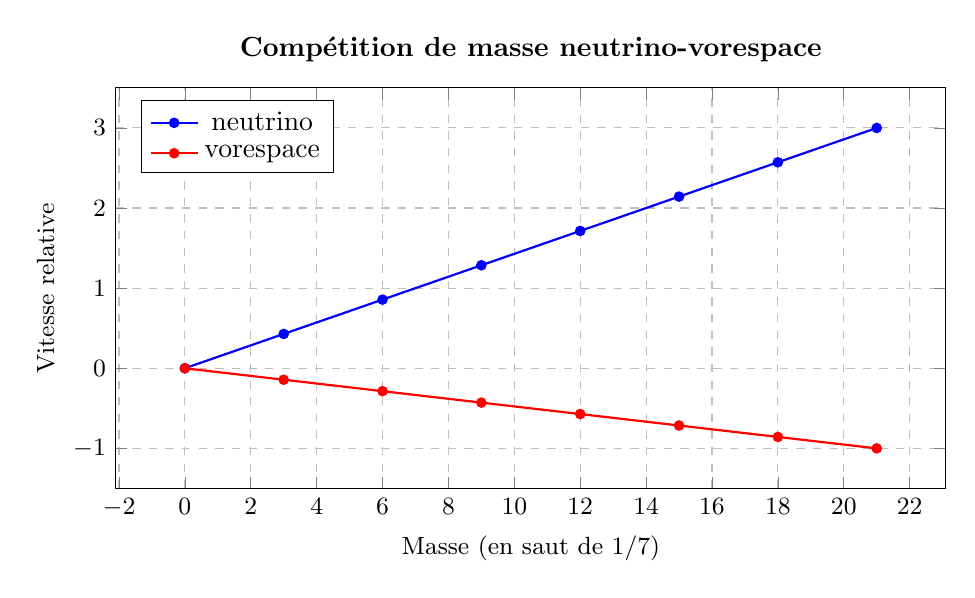
\begin{tikzpicture}
		\begin{axis}[
			width=\columnwidth,          % <-- largeur exacte de la page
			height=0.55\columnwidth,     % hauteur proportionnelle (tu peux ajuster)
			%width=14cm,
			%height=9cm,
			xlabel={Masse (en saut de 1/7)},
			%
			ylabel={Vitesse relative},
			title={Compétition de masse neutrino-vorespace},
			xmajorgrids=true,
			ymajorgrids=true,
			grid style=dashed,
			%ymode=log,                  % <--- échelle logarithmique sur l'axe y
			%log basis y=10,
			ymin=-1.5,                   % pour éviter le log(0)
			ymax=3.5,
			xlabel style={font=\small},
			ylabel style={font=\small},
			title style={font=\bfseries},
			tick label style={font=\small},
			legend pos=north west,
			]
			
			% Données (x = indice, y = valeur)
			\addplot[
			color=blue,
			thick,
			mark=*, 
			mark size=1.5pt,
			] coordinates {
				(0,0)
				(3,3/7)
				(6,6/7)
				(9,9/7)
				(12,12/7)
				(15,15/7)
				(18,18/7)
				(21,21/7)
			};
			\addlegendentry{neutrino}
			\addplot[
			color=red,
			thick,
			mark=*, 
			mark size=1.5pt,
			] coordinates {
				(0,0)
			 	(3,-1/7)
			 	(6,-2/7)
			 	(9,-3/7)
			 	(12,-4/7)
			 	(15,-5/7)
			 	(18,-6/7)
			 	(21,-7/7)
			 };   
			\addlegendentry{vorespace}
			
		\end{axis}
	\end{tikzpicture}
\end{center}
%\vspace*{-0.5cm}
\begin{center}
	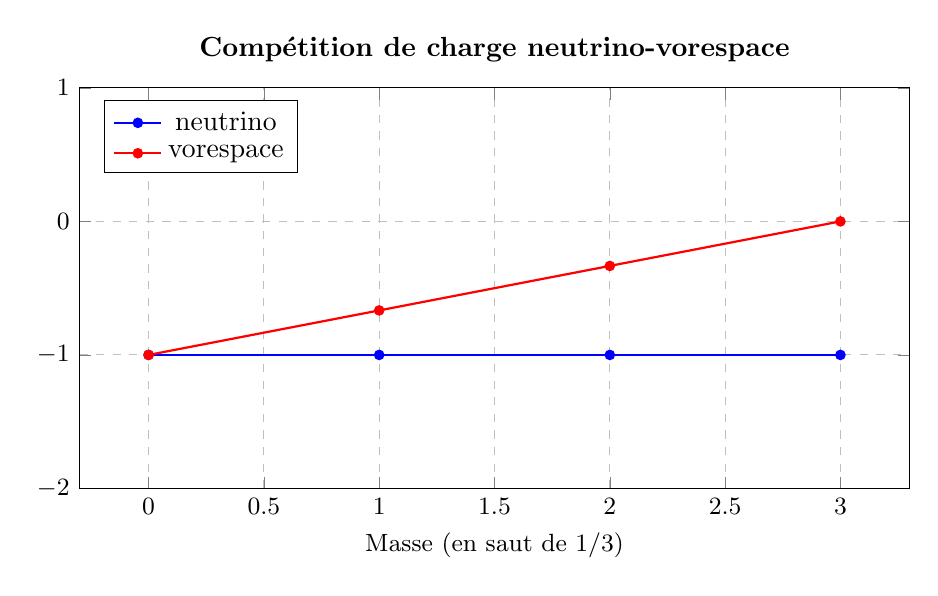
\begin{tikzpicture}
		\begin{axis}[
			width=\columnwidth,          % <-- largeur exacte de la page
			height=0.55\columnwidth,     % hauteur proportionnelle (tu peux ajuster)
			%width=14cm,
			%height=9cm,
			xlabel={Masse (en saut de 1/3)},
			%ylabel={Vitesse relative},
			title={Compétition de charge neutrino-vorespace},
			xmajorgrids=true,
			ymajorgrids=true,
			grid style=dashed,
			%ymode=log,                  % <--- échelle logarithmique sur l'axe y
			%log basis y=10,
			ymin=-2.0,                   % pour éviter le log(0)
			ymax=1.0,
			xlabel style={font=\small},
			ylabel style={font=\small},
			title style={font=\bfseries},
			tick label style={font=\small},
			legend pos=north west,
			]
			
			% Données (x = indice, y = valeur)
			\addplot[
			color=blue,
			thick,
			mark=*, 
			mark size=1.5pt,
			] coordinates {
				(0,-1)
				(7/7,-1)
				(14/7,-1)
				(21/7,-1)
			};
			\addlegendentry{neutrino}
			\addplot[
			color=red,
			thick,
			mark=*, 
			mark size=1.5pt,
			] coordinates {
				(0,-1)
				(7/7,-2/3)
				(14/7,-1/3)
				(21/7,0)
			};   
			\addlegendentry{vorespace}
			
		\end{axis}
	\end{tikzpicture}
\end{center}

Un photon étant un révélateur entropique, il va être sensible à la disparité des états internes de chacun des objets et ne pas réagir de la même façon suivant les états. Il traversera le vorespace, mais sera bloqué dans l'électron. La différence entre les deux est minimale --~c'est la constante de structure fine $\alpha$~--, mais suffisante pour changer les règles du jeu de l'interaction du photon avec les nœuds de type $S_3$.

Or la masse est duale avec le champ magnétique: c'est le flux $\Phi$ de l'électromagnétisme. On peut donc voir la répartition des valeurs de masse comme une répartition duale des valeurs de charges magnétiques du monopole associé. En ramenant les charges à des valeurs uniquement positives, on a donc:

%\vspace*{-1.0cm}
\begin{center}
	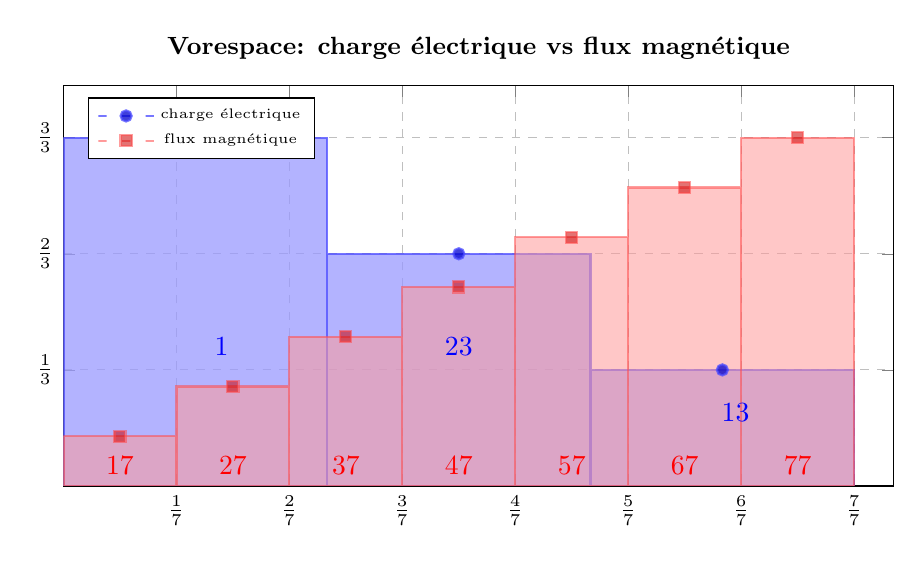
\begin{tikzpicture}
	\begin{axis}[
		width=\columnwidth,          % <-- largeur exacte de la page
		height=0.55\columnwidth,     % hauteur proportionnelle (tu peux ajuster)
		xmin=0, xmax=1.05,
		ymin=0, ymax=1.15,
		grid style=dashed,
		%xlabel={Position \( x \)},
		%ylabel={Hauteur},
		title={Vorespace: charge électrique vs flux magnétique},
		grid=major,
		legend pos=north west,
		legend style={font=\tiny},
		title style={font=\bfseries\small},
		% === Configuration de l'axe x en fractions de 1/7 ===
		xtick={1/7,2/7,3/7,4/7,5/7,6/7,7/7},
		xticklabels={
			\( \frac{1}{7} \), \( \frac{2}{7} \), \( \frac{3}{7} \), 
			\( \frac{4}{7} \), \( \frac{5}{7} \), \( \frac{6}{7} \), \( \frac{7}{7} \)
		},
		xticklabel style={font=\small}, % rotate=45, anchor=east}, % pour éviter le chevauchement
		ytick={1/3, 2/3, 3/3},
		yticklabels={
				\( \frac{1}{3} \), \( \frac{2}{3} \), \( \frac{3}{3} \), 
		},
		yticklabel style={font=\small}, 
		]
		% ==================== Série 1/3 : barres larges (largeur = 1/3) ====================
		\addplot+[ybar, bar width=1/3, fill=blue!40, draw=blue!70, thick, opacity=0.75] 
			coordinates {
				(1/6,  1)   % centre de la première barre
				(1/2,  2/3)   % centre de la deuxième barre
				(5/6,  1/3)     % centre de la troisième barre
				};
		% ==================== Série 1/7 : barres étroites (largeur = 1/7) ====================
		\addplot+[ybar, bar width=1/7, fill=red!40, draw=red!70, thick, opacity=0.55] 
			coordinates {
				(1/14, 1/7)
				(3/14, 2/7)
				(5/14, 3/7)
				(7/14, 4/7)
				(9/14, 5/7)
				(11/14,6/7)
				(13/14,1)
				};
		\legend{charge électrique, flux magnétique};
		\node[color=red] at (2/28, 0.06) {\R{1}{7}};
		\node[color=red] at (6/28, 0.06) {\R{2}{7}};
		\node[color=red] at (10/28, 0.06) {\R{3}{7}};
		\node[color=red] at (14/28, 0.06) {\R{4}{7}};
		\node[color=red] at (18/28, 0.06) {\R{5}{7}};
		\node[color=red] at (22/28, 0.06) {\R{6}{7}};
		\node[color=red] at (26/28, 0.06) {\R{7}{7}};
		\node[color=blue] at (0.2, 0.4) {1};
		\node[color=blue] at (0.5, 0.4) {\R{2}{3}};
		\node[color=blue] at (0.85, 0.21) {\R{1}{3}};
		\end{axis}
		\end{tikzpicture}
\end{center}
%\vspace*{-1.5cm}
\begin{center}
	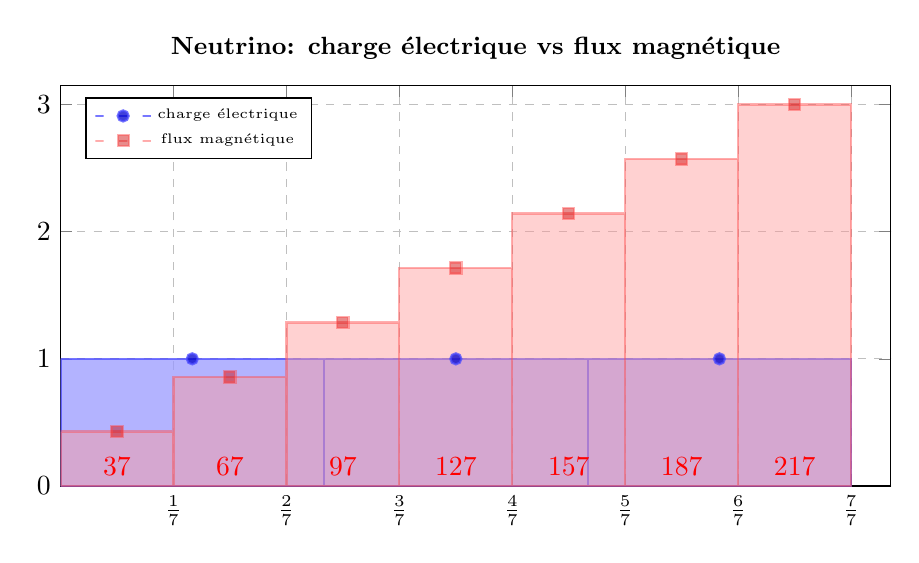
\begin{tikzpicture}
		\begin{axis}[
			width=\columnwidth,          % <-- largeur exacte de la page
			height=0.55\columnwidth,     % hauteur proportionnelle (tu peux ajuster)
			xmin=0, xmax=1.05,
			ymin=0, ymax=3.15,
			grid style=dashed,
			%xlabel={Position \( x \)},
			%ylabel={Hauteur},
			title={Neutrino: charge électrique vs flux magnétique},
			grid=major,
			legend pos=north west,
			legend style={font=\tiny},
			title style={font=\bfseries\small},
					xtick={1/7,2/7,3/7,4/7,5/7,6/7,7/7},
			xticklabels={
				\( \frac{1}{7} \), \( \frac{2}{7} \), \( \frac{3}{7} \), 
				\( \frac{4}{7} \), \( \frac{5}{7} \), \( \frac{6}{7} \), \( \frac{7}{7} \)
			},
			xticklabel style={font=\small},
			]
			% ==================== Série 1/3 : barres larges (largeur = 1/3) ====================
			\addplot+[ybar, bar width=1/3, fill=blue!40, draw=blue!70, thick, opacity=0.75] 
			coordinates {
				(1/6,  1)   % centre de la première barre
				(1/2,  1)   % centre de la deuxième barre
				(5/6,  1)     % centre de la troisième barre
			};
			
			% ==================== Série 1/7 : barres étroites (largeur = 1/7) ====================
			\addplot+[ybar, bar width=1/7, fill=red!40, draw=red!70, thick, opacity=0.45] 
			coordinates {
				(1/14, 3/7)
				(3/14, 6/7)
				(5/14, 9/7)
				(7/14, 12/7)
				(9/14, 15/7)
				(11/14,18/7)
				(13/14,21/7)
			};
			\legend{charge électrique, flux magnétique};
			\node[color=red] at (2/28, 0.15) {\R{3}{7}};
			\node[color=red] at (6/28, 0.15) {\R{6}{7}};
			\node[color=red] at (10/28, 0.15) {\R{9}{7}};
			\node[color=red] at (14/28, 0.15) {\R{12}{7}};
			\node[color=red] at (18/28, 0.15) {\R{15}{7}};
			\node[color=red] at (22/28, 0.15) {\R{18}{7}};
			\node[color=red] at (26/28, 0.15) {\R{21}{7}};	
		\end{axis}
	\end{tikzpicture}
\end{center}

Pour le vorespace, la charge magnétique est induite: elle est le résultat de la présence d'une charge électrique. En revanche, pour le neutrino, la charge magnétique est intrinsèque et la charge électrique est induite. Le neutrino est le seul véritable monopole magnétique\footnote{Un nouvel axe d'approche pour capturer des neutrinos serait de les faire dévier dans un champ magnétique.}.

Il n'est pas nécessaire, à l'instar du monopole magnétique de Dirac, d'inventer une quelconque «ligne de Dirac» pour décrire le champ du monopole, car le phonon de charge (magnétique), en tout point équivalent au phonon de masse, décrit totalement le champ.

On a ici le flux qui varie par saut entier. On a donc

\begin{equation*}
	\Phi_m = \sum_{i=1}^{7} \vec{B_i} \cdot \vec{S_i} = \mu_0 q_m
\end{equation*}
soit
\begin{equation*}
	B_i S_i = \mu_0 q_{m_i}
\end{equation*}

Or, les surfaces de pale varient proportionnellement selon un rapport de \R{1}{7}:
\begin{equation*}
	S_i = \frac{i}{7} S_0 = \frac{i}{7} \pi \frac{L_p^2}{2}
\end{equation*}

d'où
\begin{equation*}
	q_{m_i} \mu_0 = \frac{i}{7} B_i S_0
\end{equation*}

Soit
\begin{equation*}
	\left\{
	\begin{split}
		\mu_0  &\propto S_0  \\ 
		q_{m_i}&\propto \frac{i}{7} B_i 
	\end{split}
	\right.
\end{equation*}

La perméabilité magnétique est bien proportionnelle à la surface de la pale et la charge magnétique est quantifiée. On retrouve donc sans surprise la quantification de la charge magnétique de Dirac, les mesures de l'effet Hall quantique \cite{klitzing1980new} et la solution trouvée est proche du soliton de Chern-Simons \cite{jackiw1990solitons}.

\begin{center}
	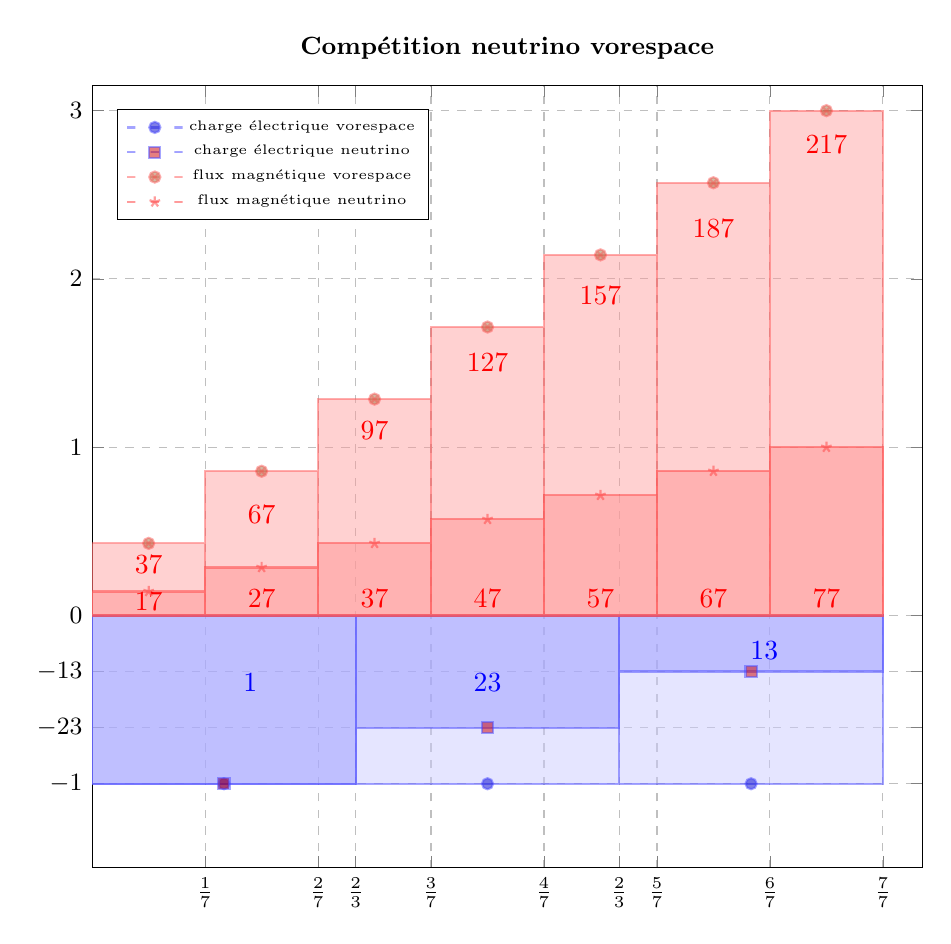
\begin{tikzpicture}
		\begin{axis}[
			width=\columnwidth,          % <-- largeur exacte de la page
			height=0.95\columnwidth,     % hauteur proportionnelle (tu peux ajuster)
			xmin=0, xmax=1.05,
			ymin=-1.5, ymax=3.15,
			grid style=dashed,
			%xlabel={Position \( x \)},
			%ylabel={Hauteur},
			title={Compétition neutrino vorespace},
			grid=major,
			legend pos=north west,
			legend style={font=\tiny},
			title style={font=\bfseries\small},
			xtick={1/7,2/7,1/3,3/7,4/7,2/3,5/7,6/7,7/7},
			xticklabels={
				\( \frac{1}{7} \), \( \frac{2}{7} \), \( \frac{2}{3} \), \( \frac{3}{7} \), 
				\( \frac{4}{7} \), \( \frac{2}{3} \), \( \frac{5}{7} \), \( \frac{6}{7} \), 
				\( \frac{7}{7} \)
				},
			xticklabel style={font=\small},
			ytick={-1, -2/3, -1/3, 0, 1, 2, 3},
			yticklabels={
					\( -1 \), 	\( \Ru{-}{2}{3}{} \), \( \Ru{-}{1}{3}{} \),
					\( 0 \),  \( 1 \), \( 2 \), \( 3 \),
				},
			yticklabel style={font=\small},	
			]
			% ==================== Série 1/3 : barres larges (largeur = 1/3) ====================
			\addplot+[ybar, bar width=1/3, fill=blue!20, draw=blue!70, thick, opacity=0.5] 
			coordinates {
				(1/6,  -1)   % centre de la première barre
				(1/2,  -1)   % centre de la deuxième barre
				(5/6,  -1)     % centre de la troisième barre			
			};
			\addplot+[ybar, bar width=1/3, fill=blue!40, draw=blue!70, thick, opacity=0.5] 
			coordinates {
				(1/6,  -1)   % centre de la première barre
				(1/2,  -2/3)   % centre de la deuxième barre
				(5/6,  -1/3)     % centre de la troisième barre
			};
			% ==================== Série 1/7 : barres étroites (largeur = 1/7) ====================
			\addplot+[ybar, bar width=1/7, fill=red!40, draw=red!70, thick, opacity=0.45] 
			coordinates {
				(1/14, 3/7)
				(3/14, 6/7)
				(5/14, 9/7)
				(7/14, 12/7)
				(9/14, 15/7)
				(11/14,18/7)
				(13/14,21/7)
			};
			\node[color=red] at (2/28, 0.3) {\R{3}{7}};
			\node[color=red] at (6/28, 0.6) {\R{6}{7}};
			\node[color=red] at (10/28, 1.1) {\R{9}{7}};
			\node[color=red] at (14/28, 1.5) {\R{12}{7}};
			\node[color=red] at (18/28, 1.9) {\R{15}{7}};
			\node[color=red] at (22/28, 2.3) {\R{18}{7}};
			\node[color=red] at (26/28, 2.8) {\R{21}{7}};	
			% == vorespace ==
			\addplot+[ybar, bar width=1/7, fill=red!40, draw=red!70, thick, opacity=0.55] 
			coordinates {
				(1/14, 1/7)
				(3/14, 2/7)
				(5/14, 3/7)
				(7/14, 4/7)
				(9/14, 5/7)
				(11/14,6/7)
				(13/14,1)
			};
			\legend{charge électrique vorespace, charge électrique neutrino, flux magnétique vorespace, flux magnétique neutrino, };
			\node[color=red] at (2/28, 0.08) {\R{1}{7}};
			\node[color=red] at (6/28, 0.1) {\R{2}{7}};
			\node[color=red] at (10/28, 0.1) {\R{3}{7}};
			\node[color=red] at (14/28, 0.1) {\R{4}{7}};
			\node[color=red] at (18/28, 0.1) {\R{5}{7}};
			\node[color=red] at (22/28, 0.1) {\R{6}{7}};
			\node[color=red] at (26/28, 0.1) {\R{7}{7}};
			\node[color=blue] at (0.2, -0.4) {1};
			\node[color=blue] at (0.5, -0.4) {\R{2}{3}};
			\node[color=blue] at (0.85, -0.21) {\R{1}{3}};
		\end{axis}
	\end{tikzpicture}
\end{center}

Comment déterminer désormais la constante de structure fine? On note deux faits troublants. En premier lieu, la valeur de cette constante est étonnamment proche de la masse du neutrino ($7,2\cdot10^{-3}$ vs $7,6\cdot10^{-3}$). Par ailleurs, la «constante» de structure fine n'est pas$\ldots$ constante. Elle varie en effet logarithmiquement en grossissant pour le boson Z\cite{workman2022review}. Si l'on extrapole les mesures expérimentales des constantes de l'électron et du boson Z\footnote{En prenant $\alpha_{e^-}=7,297\cdot10^{-3}$ et $\alpha_{Z}=7,815\cdot10^{-3}$, on obtient la droite $y=6,475\cdot10^{-5}\log_2{x}+5,743\cdot10^{-3}$, où $\log_2$ est le logarithme de base 2.} en traçant une courbe logarithmique, on obtient:
	
\begin{center}
	\begin{tikzpicture}
		\begin{axis}[
			xmode=log,
			log basis x=2,                  % échelle logarithmique en base 2
			xmin=2^0, xmax=2^36,           % plage en x
			ymin=0.0055, ymax=0.0082,
			xlabel={Nœuds},
			ylabel={},
			title={Constantes de structure fine\\ (échelle logarithmique)},
			grid=major,
			xmajorgrids=true,
			ymajorgrids=true,
			grid style=dashed,
			title style={align=center, font=\bfseries},
			width=0.95\columnwidth,          % <-- largeur exacte de la page
			height=0.55\columnwidth,     % hauteur proportionnelle (tu peux ajuster)
			% Formatage des ticks en puissance de 2
			xtick={2^0, 2^8, 2^16, 2^24, 2^32, 2^36},
			xticklabels={
				\(\underset{neutrino}{1}\), \(8\), \(16\), 
				\(\underset{\acute{e}lectron}{24}\), \(\underset{boson\ Z}{32}\), \(36\),
			},
			xticklabel style={font=\small},
			ytick={ 0.005, 0.006, 0.007, 0.008},
			yticklabels={
			    \(0.005\), \(0.006\), 
				\(0.007\), \(0.008\),
			},
			yticklabel style={font=\small},
			scaled y ticks=false,
			]
			% Points exacts
%			\addplot[blue,	mark=*,] coordinates {
%			%	(2^0, 0.00565)
%				(2^24, 0.0073)
%				(2^32, 0.0078)
%			};
			\addplot[blue, thick, domain=2^0:2^32] 
			{6.25e-5 * log2(x) + 0.0058};
			\addplot[blue, only marks, mark=*, mark size=1.5pt] 
			coordinates {
				(2^0, {0.0000625 * log2(2^0) + 0.0058})
				(2^8, {0.0000625 * log2(2^8) + 0.0058})
				(2^16, {0.0000625 * log2(2^16) + 0.0058})
				(2^24, {0.0000625 * log2(2^24) + 0.0058})
				(2^32, {0.0000625 * log2(2^32) + 0.0058})
			};
		\end{axis}
	\end{tikzpicture}
\end{center}

Il existe donc une constante par nœud du plenum (celle du neutrino valant approximativement $5,743\cdot10^{-3}$, soit environ $1/174$), ce qui n'a rien en soi d'extraordinaire, car la contante mesure l'effet de masse (ou du magnétisme) des constituants d'un nœud par rapport au modèle du vorespace (uniquement chargé électriquement). Que l'effet suive une loi logarithmique est donc intrinsèque à la \PQ.

Regardons comment évoluent ces constantes en calculant leurs valeurs approximatives, à partir de la droite calculée expérimentalement.

\vspace*{-0.5cm}
\begin{center}
	\begin{longtblr}[
		%theme=widecaption 
		caption={\footnotesize{\textbf{Calcul des valeurs approximatives des constantes de structure fine}}},
		label = {tblr:5-0-3},
		]{
			colspec={Q[c,m]  Q[2.2cm,c,m] Q[3.5cm,c,m] },
			rowspec={Q[c,m]},
			row{odd}={bg=blue!10!white},
			row{1}={c,mode=text,fg=white,bg=pkcolor, cmd=\textbf}, %cmd=\textbf, blue!80!orange
			rowsep=2pt, colsep=3pt,
			vline{2-Y} = {1}{0.3pt,gray!50},
			vline{2-Y} = {2-Z}{0.3pt,gray!30},
			hline{Z} = {0.1pt,blue},
			% nombre de col début et fin qui apparaissent à chaque page
			% 1 pour le titre par exempel
			rowhead = 1, %rowfoot = 1, 
		}		
		Nœuds  &   $\alpha$               &  Rapport (approximatif)   \\
          1    & 5,743$\cdot 10^{-3}$     &     1/174                 \\
          8    & 6,261$\cdot 10^{-3}$     &     1/160                 \\ 
         16    & 6,779$\cdot 10^{-3}$     &     1/148                 \\ 
         24    & 7,297$\cdot 10^{-3}$     &     1/137                 \\
         32    & 7,815$\cdot 10^{-3}$     &     1/125                 \\
         40    & 8,333$\cdot 10^{-3}$     &     1/120                 \\
         48    & 8,851$\cdot 10^{-3}$     &     1/113                 \\
         56    & 9,369$\cdot 10^{-3}$     &     1/107                 \\
         64    & 9,887$\cdot 10^{-3}$     &     1/101                 \\          
	\end{longtblr}
\end{center}

On «sent» donc qu'il existe une loi de construction logarithmique à base de $2^8$ et on «sent» aussi que cette loi agit fractalement, d'abord dans le nœud, puis dans la série des nœuds. On a déjà une telle loi, naturellement, de par la masse (ou le magnétisme), en interne. L'extrapoler en externe n'est pas coûteux, car c'est très ockhamien.

En calculant les rapports de deux constantes de structure fine consécutives, on se rend compte que la valeur varie très peu, sans doute uniquement à cause des approximations précédentes. Il est donc judicieux de choisir la valeur qui correspond aux variables connues, comme l'électron et le boson Z, ce qui donne une valeur d'environ 1,07, soit $1 + \R{7}{100}$. En appelant $\Phi$ cette valeur, on en déduit la loi de variation logarithmique des constantes de structure fine:
\begin{equation}
	\label{eq:structure-fine}
	\alpha_{S_i} = \Phi^i \alpha_{S_0}, \text{ i variant de 0 à 8.} 
\end{equation}

Étudions l'action du vorespace et du neutrino. Dimentionnellement, l'action des systèmes suit le produit de la charge électrique et de la charge magnétique (Weber $\times$ Coulomb, soit $Wb\cdot C=V\cdot s \cdot A \cdot s = kg \cdot m^2 \cdot s = J \cdot s$). On peut donc tracer l'évolution des actions, en considérant que la charge magnétique est proportionnelle au flux (et donc que l'échelle de l'action du neutrino n'est pas respectée):
\vfill

\clearpage
\begin{center}
	\begin{longtblr}[
		%theme=widecaption 
		caption={\footnotesize{\textbf{Actions du vorespace et du neutrino}}},
		label = {tblr:10-0-2},
		note{a}  = {à une constante multiplicative près.},           % ← Définition de la note
		]{
			colspec={Q[c,m] Q[3.5cm, c,m] Q[3.5cm,c,m] },
			rowspec={Q[c,m]},
			row{odd}={bg=blue!10!white},
			row{1}={c,mode=text,fg=white,bg=pkcolor, cmd=\textbf}, %cmd=\textbf, blue!80!orange
			rowsep=2pt, colsep=3pt,
			vline{2-Y} = {1}{0.3pt,gray!50},
			vline{2-Y} = {2-Z}{0.3pt,gray!30},
			hline{Z} = {0.1pt,blue},
			% nombre de col début et fin qui apparaissent à chaque page
			% 1 pour le titre par exempel
			rowhead = 1, %rowfoot = 1, 
		}		
		Pas       &   Vorespace     &  Neutrino \TblrNote{a}   \\
		\R{1}{7}  &    \R{1}{7}     &   \R{3}{7}  \\
		\R{2}{7}  &    \R{2}{7}     &   \R{6}{7}  \\
		\R{3}{7}  &    \R{5}{63}    &   \R{9}{7}  \\
		\R{4}{7}  &    \R{8}{21}    &   \R{12}{7} \\
		\R{5}{7}  &    \R{5}{63}    &   \R{15}{7} \\
	    \R{6}{7}  &    \R{2}{7}     &   \R{18}{7} \\
	    \R{7}{7}  &    \R{2}{21}    &   \R{21}{7} \\		    	
	\end{longtblr}
\end{center}
\begin{center}
	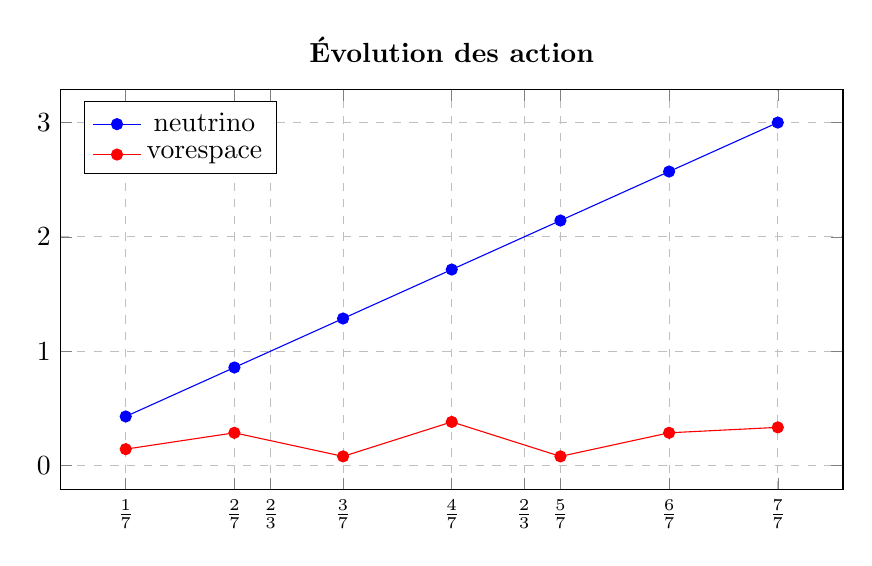
\begin{tikzpicture}
		\begin{axis}[
			%xmode=log,
			%log basis x=2,                  % échelle logarithmique en base 2
			%xmin=2^0, xmax=2^36,           % plage en x
			%ymin=0.0055, ymax=0.0082,
			xlabel={},
			ylabel={},
			title={Évolution des action},
			grid=major,
			xmajorgrids=true,
			ymajorgrids=true,
			grid style=dashed,
			title style={align=center, font=\bfseries},
			width=0.95\columnwidth,          % <-- largeur exacte de la page
			height=0.55\columnwidth,     % hauteur proportionnelle (tu peux ajuster)
			legend pos=north west,
			% Formatage des ticks en puissance de 2
			xtick={1/7,2/7,1/3,3/7,4/7,2/3,5/7,6/7,7/7},
			xticklabels={
				\( \frac{1}{7} \), \( \frac{2}{7} \), \( \frac{2}{3} \), \( \frac{3}{7} \), 
				\( \frac{4}{7} \), \( \frac{2}{3} \), \( \frac{5}{7} \), \( \frac{6}{7} \), 
				\( \frac{7}{7} \)
			},
			xticklabel style={font=\small},
			]
			% Points exacts
			\addplot[blue, mark=*,] 
			coordinates {
				(1/7, 3/7)
				(2/7, 6/7)
				(3/7, 9/7)
				(4/7, 12/7)
				(5/7, 15/7)
				(6/7, 18/7)
				(7/7, 21/7)
			};
			\addplot[red, mark=*,]
			coordinates {
				(1/7, 1/7)
				(2/7, 2/7)
				(3/7, 5/63)
				(4/7, 8/21)
				(5/7, 5/63)
				(6/7, 2/7)
				(7/7, 7/21)
			} ;
			\legend{neutrino, vorespace};
		\end{axis}
	\end{tikzpicture}
\end{center}

Il s'ensuit que, dans le cadre du monopole magnétique, l'action varie par saut d'entiers:
\begin{equation*}
	q_e q_m \propto i, \text{ i variant de 1 à 7.} 
\end{equation*}

Le processus étant fractal, ses propriétés sont invariantes par facteur d'échelle. On peut donc trouver le facteur de proportion en étudiant n'importe quel nœud similaire, en particulier l'électron. Or on a vu que l'énergie sur un cycle complet était un photon d'énergie $h$, donc d'action $h$ sur un cycle. Il s'agit ici de réduire le cycle au seul électron, donc sur un demi-cycle. On a donc
\begin{equation*}
	q_e q_m = i\frac{h}{2}, \ \text{ i variant de 1 à 7.} 
\end{equation*}

Il s'ensuit que le premier dipôle magnétique est l'association neutrino-antineutrino. Le couplage des deux phonons de charge boucle sur lui-même, créant le premier champ magnétique bipolaire.

Bien évidemment, cette structure est hautement instable et le premier nœud stable qui garde invariant le champ magnétique bipolaire est le nœud $S_1$. Le second nœud du même genre est le $S_4$, le bozon Z. Ces deux nœuds sont les hopfions décrits en page~\pageref{figure:1-hopfion} à la figure~\ref{figure:1-hopfion}. On peut désormais largement améliorer leur représentation en dessinant un tore de turbines à la place du simple tore de la figure~\ref{figure:1-hopfion}. Dans le monde macroscopique, les particules magnétiques sont bien entendu composites.

Il faut bien différencier les champs magnétiques dont on parle. Le monopole magnétique crée un champ $\vec{H}$ à potentiel central. Les nœuds de type $S_3$, des monopoles électriques, engendrent des champs magnétiques induits $\vec{B}$. Tous les autres nœuds engendrent des champs magnétiques $\vec{H}$, mais ce sont des bipoles magnétiques, donc avec des lignes de champs bouclées. On peut résumer le tout dans le tableau \ref{tblr:11-0-2}:
\end{multicols}
\vspace*{-1.0cm}
\begin{center}
	\begin{longtblr}[
		%theme=widecaption 
		caption={\footnotesize{\textbf{Structure électromagnétique des nœuds}}},
		label = {tblr:11-0-2},
		%note{a}  = {à une constante multiplicative près.},           % ← Définition de la note
		]{
			colspec={Q[2cm,c,m] Q[2.8cm,c,m] Q[2.8cm,c,m] Q[2.8cm,c,m] Q[2.8cm,c,m]},
			rowspec={Q[c,m]},
			row{odd}={bg=blue!10!white},
			row{1}={c,mode=text,fg=white,bg=pkcolor, cmd=\textbf}, %cmd=\textbf, blue!80!orange
			rowsep=2pt, colsep=3pt,
			vline{2-Y} = {1}{0.3pt,gray!50},
			vline{2-Y} = {2-Z}{0.3pt,gray!30},
			hline{Z} = {0.1pt,blue},
			% nombre de col début et fin qui apparaissent à chaque page
			% 1 pour le titre par exempel
			rowhead = 1, %rowfoot = 1, 
		}		
		Nœud        &Monopole électrique &Monopole magnétique&Dipole magnétique& Champ magnétique \\
		$S_0(-1,0)$ &    \vraiV          &   \fauxR          &    \fauxR       &       $\vec{B}$  \\
		$S_0(0,1) $ &    \fauxR          &   \vraiV          &    \fauxR       &       $\vec{H}$  \\
		$S_1(0,1) $ &    \fauxR          &   \fauxR          &    \vraiV       &       $\vec{H}$  \\
		$S_2(0,1) $ &    \fauxR          &   \fauxR          &    \vraiV       &       $\vec{H}$  \\
		$S_3(-1,1)$ &    \vraiV          &   \fauxR          &    \fauxR       &       $\vec{B}$  \\
		$S_4(0,1) $ &    \fauxR          &   \fauxR          &    \vraiV       &       $\vec{H}$  \\
		$S_5(0,1) $ &    \fauxR          &   \fauxR          &    \vraiV       &       $\vec{H}$  \\
		$S_6(-1,1)$ &    \vraiV          &   \fauxR          &    \fauxR       &       $\vec{B}$  \\
	\end{longtblr}
\end{center}

\begin{multicols}{2}
	Comme
\begin{equation*}
	\begin{split}
		[q_e q_m] &= [ \text{Action} ]                         \\
		          &= [\text{Moment cinétique}]                 \\
		          &= [\text{Quantité de mouvement}             \\
		          &\phantom{= [} \ \text{angulaire de rotation}] \\
	\end{split}
\end{equation*}
et en rapprochant l'action des nœuds et le magnétisme, il s'ensuit que le spin est \textit{l'expression du moment magnétique des nœuds de type $S_3$}. Il est donc lié tant à la présence de la charge électrique qu'à la forme des pales, leur largeur (le bi-vecteur) et leur épaisseur (tri-vecteur).

\clearpage
\begin{mybox}[breakable,colback=blue!10, colbacktitle=pkcolor]{Le spin}
	Le spin n'est pas une propriété sortie \textit{ex nihilo} de la dimension quantique. C'est l'expression du moment magnétique induit par l'excitation de la charge électrique d'un nœud de type $S_3$.
\end{mybox}

On a donc
\begin{equation*}
	S = q_e q_m = n \frac{h}{2}, \text{ n variant de 1 à 7.} 
\end{equation*}

Enfin, le spin étant à la fois colinéaire et proportionnel au flux, et multiple de la charge électrique et magnétique, il est donc le \textit{vecteur de Poynting} au niveau du nœud $S_3$:
\begin{equation*}
	\vec{S} = \vec{E} \wedge \vec{H} 
\end{equation*}

%Ainsi, $\vec{S}$ est le résultat de la combinaison de deux mouvements, l'un de rotation, l'autre de précession, le premier représentant la charge électrique et le second la charge magnétique.

%Il existe donc deux moments cinétiques à l'origine du moment cinétique de spin. Un moment cinétique de charge, qu'on appelera \textit{orbital} pour être en phase avec la \MQ, et un moment cinétique purement \textit{magnétique}, correspondant au mouvement de précession.

%Contrairement à la \MQ, la \PQ\ postule que le moment cinétique total d'un nœud $S_3$ est le moment cinétique de spin, et non la somme du moment cinétique orbital et du moment cinétique de spin. Techniquement, cela ne change pas grand-chose, mais ce renversement permet de remettre les moments dans leur ordre de préséance naturelle.

Le spin est donc la \textit{densité de flux magnétique}, c'est-à-dire \textit{la puissance du rayonnement magnétique}, dont l'origine peut être électrique (vorespace, électron) ou bien purement magnétique comme avec le dipôle magnétique qu'est le neutrino. Quoi qu'il en soit, il naît de la rotation d'un nœud et est donc étroitement lié à ce mouvement. On appelera moment cinétique \textit{orbital} $\vec{L}$ le moment cinétique dû à la rotation. $\vec{S}$ et $\vec{L}$ sont donc les deux faces d'un même mouvement, d'un côté la charge électrique, de l'autre le champ magnétique induit.

Le moment cinétique orbital $\vec{L}$ correspondant à la charge, il tourne obligatoirement par valeur entière de tour. Il varie donc par saut d'entier naturel. On appelera $l$ la valeur de ce moment.

On peut s'en persuader en revenant à la défintion d'un moment cinétique:
\begin{equation*}
	\vec{L} = \vec{r} \wedge \vec{p} 
\end{equation*} 
soit
\begin{equation*}
		l = m r^2 \omega = 2n \pi m r^2 
\end{equation*}
avec $n$ le nombre de tours et $r$ le rayon de la pale, qui dépend donc de la taille du nœud $S_i$: $r=r(i)$.

La rotation des pales induit aussi un moment cinétique purement magnétique $\vec{\mathcal{M}}$, colinéaire au moment cinétique orbital, dont il est en quelque sorte le dual. $\vec{\mathcal{M}}$ est donc proportionnel à $\vec{L}$. Il est trivial de montrer que le facteur de proportionnalité correspond au rapport gyroscopique $\gamma = q_e/2m$, le calcul et la démarche classique pouvant s'appliquer ici.

On a donc
\begin{equation*}
	\vec{\mathcal{M}} = \frac{q_e}{2m} \vec{L} 
\end{equation*} 
 

\begin{figure}[H]
	%\captionsetup{width=5cm}
	\label{figure:Moment-0}
	\centering
	
\includegraphics[width=0.8\columnwidth]{moments-cinetiques.pdf}
	\caption{\footnotesize{\textbf{Moments cinétiques des pales.} La pale (en marron clair) fait un angle avec la verticale (représentée par l'axe $(Oz)$), marque de la charge électrique. Le moment cinétique orbital $\vec{L}$ est perpendiculaire à la pale, tandis que le moment cinétique magnétique, assimilé au moment magnétique, en vert, lui est colinéaire. En orange, le flux à un endroit donné, dépend donc du rayon. Le spin est la densité de flux magnétique --~le vecteur de Poynting~--, donc la moyenne du flux sur la surface de la pale. Le flux, ainsi que le spin, est perpendiculaire à la surface. La figure n'est pas à l'échelle.}}
\end{figure}

Il faut bien se rappeler que la pale est une pale d'hélicoïde et qu'elle est mieux représentée comme suit (à l'épaisseur variable près):
\begin{center}
	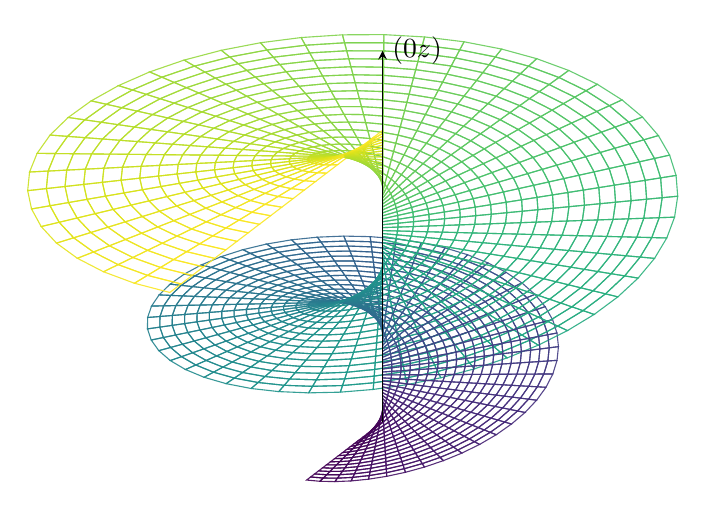
\begin{tikzpicture}
		\def\a{0.2}
		\def\b{0.25}
		\begin{axis}[
			% Configuration de la vue et des axes
			view={120}{30},     % Angle de vue (azimut, élévation)
			width=\columnwidth, height=\columnwidth,
			axis lines=none,    % Masquer les axes pour un rendu plus propre
			xmin=-8, xmax=2,
			ymin=-7, ymax=5,
			zmin=-1, zmax=4,
			% Paramètres de rendu
			colormap/viridis,   % Palette de couleurs
			]
			% Tracé de l'hélicoïde
			\addplot3 [
			%surf,               % Type de tracé : surface
			mesh,               % fil de fer
			shader=interp,      % Lissage des couleurs
			opacity=0.9,        % Transparence avec surf
			domain=0:4*pi,      % Angle (rotation)
			domain y=0:2.5,     % Rayon (extension)
			samples=100,         % Nombre d'échantillons (précision)
			samples y=20,
			] (
			{(1 + (1/7)*x)*y*cos(deg(x))},    % x = r * cos(theta)
			{(1 + (1/7)*x)*y*sin(deg(x))},    % y = r * sin(theta)
			%{\b*(x + (1 - (1/7)*x) * y * 0.577)}   % si inclinaison (tan(30°)) 
			{\b*x}
			);
			% Optionnel : Tracer l'axe central
			%\addplot3 [black, thick, domain=-0.5:3*pi, samples=2, samples y=0] 
			%(0,0,{0.2*x});
			\draw[thin, -stealth] (axis cs:0,0,0) -- (axis cs:0,0,4) node[right] {$(0z)$};
		\end{axis}
	\end{tikzpicture}
\end{center}

La \MQ\ a pris le parti de considérer l'ensemble $\vec{S}+\vec{L}$ comme caractéristique de l'objet quantique. En réalité, le spin n'est pas totalement indépendant du moment cinétique magnétique intrinsèque, car il en est la somme sur 2 tours.

En effet, si l'on considère le nœud d'un point de vue énergétique, donc du travail, on a
\begin{equation*}
	\left\{
	\begin{split}
		\delta W &= P(t) dt = S dt \\
		\delta W &= \mathcal{M} d\theta
	\end{split}
	\right.
\end{equation*}
soit
\begin{equation*}
	S = \mathcal{M} \frac{d\theta}{dt} = \mathcal{M} \omega
\end{equation*}

Comme la vitesse de rotation du vorespace est la moitié de celui du neutrino, on obtient pour toute particule massique:
\begin{equation*}
	S = 2  \mathcal{M} \omega = 2 \frac{q_e}{2 m} = g \frac{q_e}{2 m}
\end{equation*}

%


Le \textit{facteur de Landé}, sorti un peu miraculeusement des équations de Dirac\cite{dirac1928quantum}, n'est en réalité que l'expression de la masse (donc du magnétisme) des particules que l'on mesure, c'est-à-dire des particules massiques.

Or la mesure du facteur de Landé montre qu'il n'est pas rigoureusement égal à 2, mais à 2 «plus un \R{2}{1000}». Le neutrino tourne donc un peu plus vite que deux fois la vitesse du vorespace. Si le facteur était de 2, ce serait un facteur fractal qui ne changerait pas les propriétés du vorespace, à savoir que le photon «traverse» le vorespace. Mais comme le facteur est très légèrement plus grand, la géométrie de la pale est très légèrement modifiée, et le photon ne peut plus «traverser» le nœud massique: il va buter dessus en transférant sa quantité de mouvement, créant l'interaction électromagnétisme.

Notez que l'on aurait pu directement intuiter ce résultat en disant tout simplement que le flux du vorespace est moitié moindre que celui du neutrino.

Notez enfin qu'en choisissant comme nombre quantique magnétique la projection de $\vec{L}$, la \MQ\ crée une confusion entre les genres. Certes, le moment cinétique orbital est relié au magnétisme, au sens où ce dernier est induit par la rotation, mais il aurait été bien plus heureux de nommer les nombres quantiques $m_l$ comme les projections de $\vec{\mathcal{M}}$. Il sera peut-être très difficile de remettre de l'ordre, à cause des habitudes. Mais la facilité de compréhension des domaines sous-jacents y gagnerait énormément\dots
\medskip

On peut désormais relier le facteur de Landé avec la constante de structure fine. Conformément aux calculs de la \MQ, le facteur de Landé correspond à l'agrandissement du cercle magnétique. C'est donc la partie du rayon excédentaire, et on retrouve donc classiquement le fait qu'il soit proportionnel à la constante de structure fine et que son facteur de proportion soit le tour d'un cercle complet:
\begin{equation*}
	g = \frac{\alpha}{2\pi}
\end{equation*} 

La masse, ou le magnétisme, induit donc une transformation plus subtile qu'un simple élargissement de la surface de la pale et de son épaisseur: elle induit un gonflement de l'épaisseur qui s'arrondit, un peu sur le modèle d'une chambre à air. Cet allongement, par rapport à l'épaisseur, est exactement le facteur de Landé, soit environ \R{2}{1000}.

Ce surplus rend le passage du photon impossible. Là où il passait en éfleurant le vorespace, la surépaisseur des nœuds massiques le bloque, induisant mécaniquement une interaction entre les photons et les nœuds de type $S_3$.

En outre, le rayon de la pale étant proportionnelle à la taille du nœud, on retrouve la loi logarithmique de la constante de structure fine \eqref{eq:structure-fine}.

Enfin, la vitesse apparente du neutrino, double du vorespace, ne doit pas cacher que seule la pale magnétique porte la vitesse réelle, soit le triple de la vitesse de celle du vorespace. Le surplus de vitesse s'applique par conséquence uniquement à cette pale, qui tourne donc un peu plus vite que 3. Pour l'électron, elle tourne à 3,002\,319\,304, soit un peu plus de 7\,~\% que la vitesse théorique. On retrouve bien le saut d'un peu plus de \R{7}{100} énoncé dans la loi fractale.
\medskip

Malheureusment, je n'ai pas été capable de calculer la valeur exacte de $g$ (ou de $\alpha$). Soit cela nécessite un esprit plus astucieux, soit cette constante est instrinsèque au plenum, et est donc la seule véritable constante fine de l'univers. Le modèle du Big Bang proposé plus bas peut faire pencher en faveur de cette hypothèse: il s'agirait du réglage exact correspondant à la quantité d'énergie nécesaire à la création du neutrino qui permet de développer l'interaction électromagnétisme dans l'univers.\footnote{Le fait que ce soit la seule «anomalie» rigoureusement non démontrable  chiffonne l'auteur. Toute la \PQ\ est structurellement mécanique et explicable, et cela devrait  aussi être  le cas ici. S'il est exact qu'il est impossible de calculer cette constante, alors elle serait effectivement le seul réglage fin de l'univers.}

\subsubsection{Les autres constantes de la physique}

Il faudrait prendre le temps de reconstruire toutes les constantes de
la physique, même si, à ce stade, on peut très bien tout reconstruire
mécaniquement avec celles déjà trouvées, car c'est \textit{grosso modo} ce que
fait la physique actuellement.

Il faut remarquer qu'une constante n'a aucun sens réel, c'est la
charge de Planck. C'est un simple effet de bord de l'extrapolation des
unités de Planck à toutes les caractéristiques de la physique: en
postulant une charge de Planck et en la définissant comme charge
élémentaire portée par une particule de Planck, une particule de la
taille de Planck. On a donc une impossibilité physique de représenter
une telle particule, sauf à l'associer à deux vorespaces ou à deux
neutrinos. La définition précédente renvoie au rayon de Schwarzschild,
c'est-à-dire à la masse maximale d'un objet, donc il s'agirait plutôt
d'un assemblage de neutrinos. Or, par définition, les neutrinos n'ont
pas de charge!

\section{Équivalence de la plénodynamique quantique avec la physique actuelle}

\subsection{Introduction} 

Il est nécessaire de s'assurer que la \PQ\  est compatible avec toute la
physique, si elle veut prétendre être une physique du tout. Elle s'est
construite sur la mécanique et sur la thermodynamique, ainsi que
sur l'électromagnétisme. Elle est déjà compatible avec ces théories.
Il faut toutefois encore passer l'épreuve des trois grandes théories
de la physique, à savoir les relativités restreinte et générale, ainsi que
la mécanique quantique.

\subsection{Relativité restreinte}

En ce qui concerne la relativité restreinte, c'est la partie la plus
facile, car la \PQ\ s'est construite justement en respectant les bases de
la relativité restreinte, à savoir un transfert d'information basé
sur la vitesse de la lumière comme vitesse maximale.

D'une certaine façon, la \PQ\ peut être vue comme le pendant réel de la
relativité restreinte, qui se trouve d'ordinaire être un cadre
général, valide partout. La \PQ\ incarne donc la relativité restreinte.

Il est aisé de retrouver le facteur de Lorentz dans une particule en
déplacement. Son évolution en chenille marque une différence entre le
début de son déplacement et la fin, que l'on peut triangulariser dans
un triangle rectangle qui permet alors d'extraire le facteur de
Lorentz.

Le temps ne se dilate pas à proprement dit, mais le temps de
recollement de la chenille s'allonge, car le chemin à parcourir est de
plus en plus grand.

De même, la tension dans la chenille augmente avec la vitesse, ce qui
donne en échange une augmentation de la masse, proportionnelle à cette
tension.

La \PQ\ est donc pleinement compatible avec la relativité restreinte:
on peut même dire que la \PQ\ \textbf{est} la relativité restreinte.

\subsection{Relativité générale}

Une part du travail a aussi déjà été réalisée dans le cadre de la
relativité générale. Ainsi, dans la théorie d'Einstein, une
masse courbe l'espace-temps et dans la \PQ, une masse agit sur le plenum
en lui imprimant une onde de cisaillement, le phonon de masse.

Là où Einstein montre que la lumière suit une géodésique de
l'espace-temps, le photon du plenum épouse le phonon de masse, en tant
que surfeur entropique. Il remonte les talwegs d'entropie, qui se
dirigent vers les masses.

Dans l'espace-temps d'Einstein, à proximité d'une masse, le temps
ralentit. Dans le plenum, le phonon de masse diminue les capacités de
transfert entropique, pénalisant le temps de transfert: plus le
phonon est massif, et plus le temps de transfert est pénalisé. La
masse agit bien comme un ralentisseur de temps autour d'elle.

Enfin, la relativité générale postule l'équivalence entre la masse
inerte et la masse grave. En \PQ, la masse grave est la masse du
vorespace, la tension qu'on peut appliquer à une turbine. La masse
inerte est celle engendrée par l'inertie de ce vorespace. Par
construction, elles sont identiques.

La \PQ\ est donc pleinement compatible avec la relativité générale.

\subsection{Mécanique quantique}

\subsubsection{Introduction}

On entre ici dans l'ultime étape. Si l'on peut prouver l'équivalence
entre la \PQ\ et la mécanique quantique, on aura alors uni les trois
grandes physiques et la \PQ\ sera définitivement compatible avec une
physique du tout.

On achèvera cette partie par la construction du modèle de l'atome
selon le point de vue de la \PQ, modèle qui permettra non seulement
de modéliser l'atome, mais aussi d'expliquer pourquoi il fonctionne
ainsi.

\subsubsection{La dualité onde-corpuscule}

Il va de soi que le phonon de masse et de charge (si besoin) autour
d'une particule constitue la fameuse onde des particules quantiques.
Elle n'est plus du tout mystérieuse, puisqu'il s'agit simplement de
l'interaction d'une masse, un corpuscule donc, avec le plenum.

Cette onde a néanmoins des propriétés intéressantes. C'est une onde
stationnaire heptagonale composite, au sens où elle est à la fois la
somme des ondes de chacun des sous-nœuds de la particule et de la
rotation de la particule elle-même.

Ainsi, dans le cadre de l'électron par exemple, composé de $2^{24}$ neutrinos, elle
est la composition de $2^{24}$~mini-ondes heptagonales mélangées à une onde
heptagonale de l'électron lui-même. \textit{Techniquement, l'onde n'est donc
pas composée d'une infinité d'ondes, mais d'un nombre fini.} Bien
entendu, la composition rend ce nombre «assez grand», ce qui rend
l'approximation «infinie» comme acceptable dans un premier temps.

À noter que l'onde définit entièrement la position de la particule. On
pourrait étudier seulement l'onde et rendre compte des
caractéristiques de la particule. De ce point de vue, l'onde
«pilote» bien la particule, ce qui était le point de vue de Louis de
Broglie.\cite{debroglie1924recherches}

Toutefois, c'est bien la particule qui donne naissance à l'onde et il
est plus juste de dire que \textit{la particule pilote l'onde}. Ce n'est donc
pas \textit{stricto sensu} une onde-pilote, mais plutôt une \textbf{particule-pilote},
si l'on veut garder la terminologie de Louis de Broglie.


À noter une différence majeure entre les deux théories: le
déterminisme est absolu en \PQ. Il «suffit» de calculer à quoi
ressemble l'onde pour déterminer à quoi ressemble la particule, et
vice-versa: l'une et l'autre étant en relation d'équivalence totale,
en bijection diraient les mathématiciens, il suffit de connaître l'une
pour tout savoir de l'autre.

Cette équivalence répond à la grande question quantique de ce que
représente exactement la fonction d'onde. L'école de Copenhague
affirme qu'elle contient en germes tout ce qu'il est possible de
connaître des propriétés de la particule quantique. C'est exact, au
sens où elle est engendrée par la particule quantique en question,
selon une relation déterministe qui tient compte de tous ses états. La
mécanique quantique part de cette fonction d'onde comme
référence de l'information, alors que la référence réelle est la
particule. En quelque sorte, la mécanique quantique suit un objet
éclairé par le soleil en suivant son ombre. Quand la mécanique
quantique mesure l'ombre, elle tourne alors son regard vers l'objet,
et affirme que l'ombre s'est transformée --~effondrée~-- en l'objet.
En réalité, \textit{la mesure quantique est juste un changement de point de
vue.}

Enfin, on a vu précédemment que la dualité onde-corpusculaire et la
quantification de l'impulsion entraînaient mécaniquement la formule de
de Broglie.

\subsubsection{Le cas du photon}

Le photon, notre surfeur entropique, pose un réel problème. Par
construction, il n'est qu'une onde. La dualité ne s'applique pas à son
cas, ce qui est pour le moins embêtant pour Albert Einstein qui a reçu
son prix Nobel après avoir expliqué le seuil de l'effet
photoélectrique par la présence de corpuscules de lumière!

En effet, la \PQ\ assume totalement changer le statut du photon en
physique. De même qu'elle a expliqué la nature réelle et la provenance
du photon, elle assume que le photon n'est qu'une onde pure.

La question qui se pose alors immédiatement est comment expliquer que
des milliers d'expériences de physique au cours de ces dernières
années mettent en évidence la double nature du photon? La réponse est
contenue dans la question: ce n'est pas la nature du photon que les
expériences mesurent, mais$\ldots$ les instruments eux-mêmes. Ainsi, quand
un photon se rapproche d'un détecteur physique, ce dernier, par sa composition
atomique, influe sur le plenum en créant un phonon de
masse, et même parfois de charge. Le photon, en tant que surfeur
phonique, «obéit» immédiatement au changement du plenum, créant
l'illusion qu'il est lui aussi doté d'une double-nature.

C'est peut-être la plus grosse révolution apportée par la \PQ: les
physiciens mesurent en réalité leurs instruments depuis des années
quand ils mettent en œuvre des photons!

\subsubsection{Le rôle de la mesure}

Voilà une transition toute trouvée pour examiner le rôle de la
mesure. Indépendamment du cas particulier du photon, qui est pourtant
l'acteur privilégié de la physique expérimentale actuelle, il faut se pencher
sur la notion de mesure en général.

En \MQ, la mesure impacte l'état du système, le réduisant à un état
propre, celui mesuré. La \MQ\ postule qu'un état quelconque de tous les
états superposés a été tiré au sort, selon un véritable hasard. Le
système est alors irrémédiablement réduit dans l'état mesuré.

On a vu ci-dessus qu'en réalité, la mesure quantique est un changement
de point de vue. Il n'y a pas d'écroulement de fonction d'onde, pour
la bonne raison que la nature révèle le réel et le réel est l'objet,
pas sa relation avec l'éther, même si cette relation peut
indirectement le définir. Il va de soi que lorsque les physiciens mesurent un
électron, c'est bien l'objet \node{$S_3(-1,1)$} qu'ils s'attendent à voir et à
mesurer, pas l'onde heptagonale qui l'entoure, même si cette dernière
n'est pas sans conséquence sur la mesure.

On a vu en effet que la mesure n'est pas sans impact au
niveau de la \PQ. En effet, les instruments de mesure, macroscopiques
par essence, ont un impact direct sur le plenum. \textit{Ils ne sont donc pas
neutres}. Pour expérimenter réellement, le physicien doit retirer le biais introduit par l'instrument lui-même.
Il sera compliqué de s'affranchir totalement de ce biais, quand on
mesure des objets de la taille quantique.

Reprenons par exemple le cas classique des interférences de l'électron
à travers deux fentes. L'électron possède une onde, c'est certain.
Elle peut très avantageusement interférer entre deux ouvertures,
forçant le passage de l'électron dans l'une plutôt que dans l'autre.

Mais quelle est la part du phonon de masse de chaque ouverture dans cette
histoire? Autour des deux ouvertures se créent deux couloirs de
phonon$\ldots$ Est-on certain que chaque ouverture est atomiquement
rigoureusement le miroir de l'autre (sinon, leur phonon de masse
risque de différer et, donc, de favoriser une mesure plutôt qu'une
autre)? De plus, il faut être certain de «taper pile au milieu des
fentes», car le lancer d'électron est déterministe en \PQ.
C'est-à-dire qu'en théorie, en lançant de façon identique les
électrons, ces derniers devraient suivre exactement la même trajectoire et
tous passer par le même trou. Bien entendu, il suffit de n'importe
quoi en cours de trajectoire pour changer un micro-paramètre et
changer le résultat final. Or l'air ambiant est rempli
d'interférences!

Bien entendu, la statistique vient comme bien souvent sauver l'expérience:
étant donné le grand nombre de paramètres incontrôlables, on peut
estimer raisonnable qu'ils s'annihilent statistiquement. On devrait donc retrouver
une justesse expérimentale via la statistique.

Quoi qu'il en soit, la question se pose de ce que l'on mesure
réellement aujourd'hui en physique$\ldots$ au moins au niveau quantique
quand on travaille sur les interférences.

Il va de soi que dès que le phonon de masse ou de charge peut avoir
une incidence dans une quelconque mesure, il faut en tenir compte, ne
serait-ce que pour prendre de la distance avec le résultat.

\subsubsection{L'intrication: le leurre du hasard}

Le fameux article EPR\cite{einstein1935can} d'Einstein, de Podolsky et de Rosen a lancé un
débat qui a pris fin récemment, mais que la \PQ\ se propose de relancer,
avec une conclusion inattendue. L'expérience postule que si la \MQ\ est
juste, alors il existe un état d'intrication entre deux particules et
que cet état viole la relativité restreinte, puisque l'information qui
circule entre les deux particules circulerait plus vite que la vitesse
de la lumière. L'expérience d'Aspect\cite{aspect1982experimental} a montré que cette affirmation
était vérifiée.

Pourtant, la \PQ\ affirme que le déterminisme existe et que, de fait,
l'intrication n'existe pas. Il s'agit simplement d'un effet de bord de la
théorie de la mécanique quantique, qui n'est pas la représentation la plus simple de
la réalité, mais une théorie plus complexe, comme évoquée par Poincaré\cite{poincare:1902:sh}.

La mécanique quantique emprunte donc un chemin indirect pour exprimer les
effets quantiques. Le chemin de la \PQ, plus direct, ne possède
pas les effets de bord de la mécanique quantique.

En effet, la mécanique quantique cache ce qu'elle ne connaît pas sous le
nom de hasard quantique. N'étant pas capable de calculer les
caractéristiques réelles d'une particule quantique, elle a élaboré
une technique divinatoire, excellente au demeurant, pour expliquer le
comportement des objets quantiques. Mais cette technique postule
l'idée d'un hasard irréductible, donc d'un indéterminisme structurel,
qui n'est pas le reflet de la réalité.

Prenons l'exemple de deux électrons d'un atome d'hélium. Ils sont
intriqués, au sens où chacun possède un spin opposé à l'autre. La \MQ\
affirme que seule la mesure lève cette indétermination. En réalité, il
n'y a pas d'indétermination: chaque électron possède réellement un
spin opposé à l'autre. Si vous en mesurez un, vous ne changez pas la
valeur de l'autre. L'intrication est une conséquence de la structure
(que l'on expliquera dans le modèle de l'atome), pas de la mesure.
L'intrication n'existe donc pas selon le point de vue de la
plénodynamique quantique. Vous pouvez déplacer deux objets intriqués
chacun à un bout de l'univers, en mesurer un, aucune information ne
circulera vers l'autre: les deux valeurs sont déterminées avant la
mesure.

Ainsi, l'article EPR qui supposait que la mécanique quantique fût
juste pour postuler la suite reste exact: c'est juste que l'hypothèse
de départ, la justesse de la \MQ, n'est pas conforme au réel. La
mécanique quantique utilise un hasard non réaliste qui a des
conséquences dans la mécanique quantique, pas dans la réalité.
L'intrication existe dans la mécanique quantique, pas dans la réalité,
car la mécanique quantique ne représente pas le réel, mais un moyen
mathématique et compliqué de décrire le réel. C'est une superbe illustration 
des dangers de l'utilisation des mathématiques pour décrire la physique, tel que l'énonçait de Broglie\cite{debroglie1976physique}.

Alors, comment se fait-il que l'expérience d'Aspect soit juste? Pour
exactement la même raison que les expériences sur les photons sont
justes: elles ne mesurent pas l'intrication \textit{in se}, mais l'interaction
des photons avec les instruments. Pour palier cette interférence des
capteurs, ici des lames, il faudrait mesurer les photons avec des
objets de la même nature que le photon lui-même. Sacré défi!

Quoi qu'il en soit, cela ne retire en rien à Alain Aspect d'avoir réalisé
cette expérience hors du commun.

\subsubsection{Le principe d'exclusion de Pauli}

Le principe d'exclusion de Pauli postule que deux fermions au même
endroit ne peuvent avoir des caractéristiques identiques. Ce principe
découle naturellement de la structure $S_3$ des fermions qui, pour être
ensemble, doivent avoir des caractéristiques physiques compatibles:
par exemple, pour assembler 2 $S_3$, il faut en retourner un, donc
inverser son spin, afin que les sens de vissage soient compatibles. Ce
principe est donc structurel dans la \PQ.

On verra dans le modèle de l'atome une raison plus fine de ce principe
qui découle en réalité de la minimisation de l'énergie des électrons dans les orbites atomiques.

\subsubsection{Théorème CPT}

La conservation CPT est structurellement conservée dans un nœud $S_3$
par la symétrie des 64 premiers états et des 64 suivants. L'inversion
de chiralité oblige à passer par tous les états intermédiaires. La
symétrie CPT est assurée par la structure de la turbine.

Quoi qu'il en soit et quels que soient les nœuds, la structure à 128
états est structurellement compatible avec la conservation CPT.

\subsubsection{Le principe d'indétermination d'Heisenberg}

La \PQ\ ne remet pas en cause le principe d'indétermination
d'Heisenberg. Ce dernier ne dépend en effet pas de la théorie
mathématique de la mécanique quantique: c'est un constat «évident»
que deux caractéristiques liées ne peuvent être mesurées en même temps,
les temps de mesure respectifs n'étant pas compatibles entre eux.

De plus, la quantification spatio-temporelle du plenum rend trivial le
principe d'indétermination.

\subsubsection{Conclusion sur la compatibilité}

La \PQ\ et la \MQ\ sont donc pleinement compatibles. La \PQ\ permet
simplement de corriger légèrement le tir de la \MQ, dont le hasard
intrinsèque a conduit à des conclusions parfois$\ldots$ hasardeuses. Le
déterminisme retrouve son plein droit dans le monde quantique qui n'a
plus rien de bizarre, les particules quantiques ayant retrouvé une
trajectoire déterminée.

\subsection{Le modèle atomique}

\subsubsection{Introduction}

Jusqu'à aujourd'hui, la physique a constaté que l'atome existait et en
a déduit un modèle basé sur des données purement expérimentales. C'est
un cas classique d'une «loi», extrapolée à partir de constatations
expérimentales\cite{poincare:1902:sh}. Si le modèle est juste, car il colle à l'expérience,
il ne propose en revanche aucune explication du «pourquoi» les choses
fonctionnent ainsi, et notamment, il n'apporte aucune réponse à la
\textbf{grande question}: «pourquoi l'électron ne tombe-t-il pas sur le
noyau?», question qui pourrait se poser via sa version contraposée:
«pourquoi l'électron tourne-t-il sans dépenser d'énergie?» La \PQ\
se propose de résoudre cette énigme et d'apporter pour la première
fois une réponse consistante.

Sans entrer dans les détails, l'idée générale de la construction de l'atome est de
trouver un état stable naturel à partir des particules élémentaires.
Ces dernières ne sont qu'une étape avant la stabilisation finale, qui
est l'atome. La stabilisation dans le plenum est toujours assurée par
un nœud auto-similaire à $S_3$, donc, sans surprise, on va retrouver cette
structure dans l'atome. L'électron et le noyau vont jouer le rôle des
hélices et «s'emmêler» pour former un nœud de type $S_3$. Bien
entendu, à ce stade avancé des particules, la fusion ne sera physiquement 
plus possible, et le nœud $S_3$ sera fortement distendu:
l'électron et le noyau ne seront donc plus collés.

En revanche, cet espacement laisse de la place libre pour former un
enchevêtrement complexe de nœuds $S_3$ dont chaque nœud ajouté
correspondra à un atome du tableau de Mendeleïev. La nature a tant
besoin d'épouser cette forme de nœud $S_3$ pour se stabiliser que
l'ensemble des couches électroniques forme lui-même un nœud de type
$S_3$!

Alors, prêt pour le voyage au cœur de l'atome? C'est parti$\ldots$

\subsubsection{Les bases du noyau atomique}

On a vu que les quarks, pour converger vers une structure stable de
nœud de type $S_3$, s'associaient par triplet pour former un neutron et un
proton.

Techniquement, la nature aurait pu s'arrêter là, mais la présence
d'électrons va forcer les neutrons et les protons à trouver une forme
commune de nœud pour encore plus de stabilité.

On pourrait s'étonner d'inclure le neutron dans le problème, car une
bête association proton-électron suffit par exemple à assurer la
neutralité électrique. Mais cette association seule ne permet pas de
dérouler tout l'ensemble des nœuds possibles, seulement de l'initier. Le neutron va
assurer la «glue» permettant de construire cet ensemble. Pour le
moment, admettons la nécessité d'inclure le neutron pour construire le
noyau et étudions ce qu'il se passe.

La seule forme stable pour un proton et un neutron est de former un
nœud de type $S_3$, donc un enroulement de trois quarks. C'est un modèle
légèrement hybride par rapport au modèle standard du plenum qui veut qu'il y ait
seulement une double hélice. Ici, on a une triple hélice et il est
raisonnable d'admettre que l'hélice double composée des mêmes quarks
joue un rôle unique, celui de la seconde hélice dans le modèle
standard (de la \PQ!) En effet, s'il y a trois hélices, l'objet obtenu n'est plus un
spineur. Un doute persiste sur laquelle des deux hélices va travailler de
concert avec l'autre. Il est plus «ockhamien» de choisir les quarks
identiques pour jouer un rôle similaire.

Le proton et le neutron sont donc techniquement des nœuds $S_3$,
c'est-à-dire des turbines, à l'instar des vorespaces du plenum. Pour
s'associer, ils doivent donc suivre les règles des turbines, et donc
permettre l'emboîtement des pas de vis. Un neutron et un proton
doivent donc se présenter tête-bêche, afin de tourner en sens
contraire, pour ne pas se repousser. L'aspect général forme donc un
tore. Le spin de l'ensemble vaut 0.

À noter que dans la nature, il s'agit d'un nœud peu stable, d'où la
nécessité de s'unir avec un tiers pour former un nœud plus stable.
On s'arrêtera là pour le moment afin de construire notre premier
modèle d'atome, car la structure elle-même du noyau méritera ensuite
une partie dédiée.

\subsubsection{Les bases du modèle atomique}

Prenons l'exemple de l'atome d'hydrogène pour commencer: sa
simplicité apparente va puissamment nous aider à comprendre la suite.
Jusqu'à aujourd'hui, la physique considère l'atome d'hydrogène comme composé
d'une charge positive, le proton, et d'une charge négative,
l'électron. C'est juste, mais seulement en apparence. 

En réalité, le
proton n'est pas la charge opposée de l'électron: on a vu qu'il
s'agit du positon, qui est un \node{$S_3(1,1)$}. Le proton, quant à lui,
possède la \textbf{charge apparente} du positon, mais sa répartition est
totalement différente: il est composé de 2 charges \Ru{+}{2}{3}{e} et d'une
charge \Ru{-}{1}{3}{e}. Si l'on comparait la «turbine protonique» à la «turbine
positonique», elles ne se ressembleraient pas du tout. La seconde est une
turbine inversée de l'électron, donc une vis conique à l'envers,
tournant dans le sens opposé de celui de l'électron, tandis que le proton ressemble sans doute
à une vis à deux goulots, un large bien au-dessous de sa moitié et un
plus petit, juste au dessus. Surtout, il y a une énorme différence:

\textit{Les deux hélices du proton tournent simultanément.}

Il s'ensuit que le modèle classique de l'atome d'hydrogène basée sur une
pure charge électrique négative et sur une pure charge électrique positive
est faux. La charge positive est composite: elle émet deux phonons
de charge correspondant à la charge \Ru{+}{2}{3}{e} et un phonon de charge
correspondant à la charge \Ru{-}{1}{3}{e}. Si les hélices \Ru{+}{2}{3}{e} fonctionnent de
concert, on peut réduire les deux premiers phonons à un seul double,
de \Ru{+}{4}{3}{e}.

Comme les hélices sont emmêlées, alors les phonons le sont aussi. Il y
a donc interférence et il se crée un champ phonique autour du noyau,
composition des ondes heptagonales précédentes, avec des pics à \Ru{+}{4}{3}{e},
des pics à \Ru{-}{1}{3}{e} et des pics à $e$. Bien sûr, il existe toutes les
combinaisons. Globalement, il va exister des zones pseudo-circulaires
autour du proton, dans lesquelles une charge sera privilégiée.

Quand l'électron arrive dans un tel champ, il est guidé par la
thermodynamique du plenum. Il suit donc les chemins de basse énergie,
c'est-à-dire les vallées de néguentropie. Lui a sa charge négative qui
ne change pas: c'est une vraie charge $-e$. Il va donc suivre un chemin
d'équilibre entre les talwegs de \Ru{+}{4}{3}{e} et les talwegs de \Ru{-}{1}{3}{e}.
C'est un chemin de basse énergie, qui n'en consomme donc aucune:
l'électron orbite sans effort.

En revanche, il passe devant des pics de charges et il est obligé de
s'adapter devant chacune des charges: \textit{il doit donc se retourner pour
présenter une opposition de charge qui le maintient naturellement dans
la vallée de basse énergie}. L'électron oscille, et son spin alterne
à chaque fois qu'il se présente devant une nouvelle charge, les charges étant
réparties uniformément autour de la trajectoire. L'électron oscille
donc régulièrement tout le long de sa trajectoire satellitaire.

On peut encore rendre hommage à la vision de de Broglie qui avait
proposé un modèle très proche d'oscillation de l'électron au cours de
sa trajectoire, en lui donnant une longueur d'onde spécifique.\cite{debroglie1956tentative} En
réalité, encore une fois, le modèle doit être retourné: c'est la
trajectoire qui impose l'oscillation, l'électron n'oscillant pas de
lui-même, en tout cas pas dans ce cas.

Que se passe-t-il quand on ajoute un neutron? L'atome d'hydrogène
devient du deutérium et le neutron épouse le proton selon le processus
évoqué précédemment. Encore une fois, la physique actuelle «voit»
une charge nulle dans le neutron, mais si c'était le cas, ce serait un
nœud \node{$S_3(0,1)$}, une masse pure, c'est-à-dire un neutrino. Le neutron est
composé de 2 charges négatives \Ru{-}{1}{3}{e} et d'une positive \Ru{+}{2}{3}{e}. Par un
raisonnement analogue au précédent, il se forme une double hélice
bâillonnée, dont les deux fonctionnent de concert, celles de même charge
étant synchronisées. Il faut ajouter au champ précédent un nouveau qui
est la superposition des deux phonons évoqués. Fort heureusement, c'est
un champs proche, qui change peu le champ en place. Il se contente de
«resserrer» très légèrement la trajectoire.

On peut mesurer cette différence par les énergies de ionisation, en
ajoutant le tritium, avec un neutron de plus:
\end{multicols}

\vspace*{-1cm}
\begin{center}
	\begin{longtblr}[
		%theme=widecaption 
		caption={\footnotesize{\textbf{Énergie de première ionisation des trois premiers atomes}}},
		label = {tblr:5-0-4},
		]{
			colspec={Q[c,m]  Q[c,m] Q[c,m] Q[c,m] },
			rowspec={Q[c,m]},
			row{odd}={bg=blue!10!white},
			row{1}={c,mode=text,fg=white,bg=pkcolor, cmd=\textbf}, %cmd=\textbf, blue!80!orange
			rowsep=2pt, colsep=3pt,
			vline{2-Y} = {1}{0.3pt,gray!50},
			vline{2-Y} = {2-Z}{0.3pt,gray!30},
			hline{Z} = {0.1pt,blue},
			% nombre de col début et fin qui apparaissent à chaque page
			% 1 pour le titre par exempel
			rowhead = 1, %rowfoot = 1, 
		}
		
	Isotope               &  Composition                  &  Énergie d'ionisation &    Écart/Protons seuls  \\
	Hydrogène (\ce{^1H}) H&    1 proton                   &       13,59844 eV     &             --          \\
	Deutérium (\ce{^2H}) D&  1 proton + 1 neutron         &       13,60215 eV     &      $+0,00371\,eV$     \\
	Tritium   (\ce{^3H}) T&  1 proton + 2 neutrons        &       13,60338 eV     &      $+0,00494\,eV$     \\
	\end{longtblr}
\end{center}


\begin{multicols}{2}
C'est une confirmation. La trajectoire ne change globalement pas et
subit un léger effet correctif, à chaque ajout de neutron.
\medskip

Que se passe-t-il désormais quand on ajoute un proton? L'atome
devient de l'hélium avec deux protons et un neutron. On verra dans la
partie suivante comment s'arrange le noyau pour valider cette
association. On admet seulement à ce stade que le neutron sépare les
deux protons de façon à les isoler l'un de l'autre, en évitant autant
que possible leur répulsion. Le double emboîtement proton + neutron
inversé + proton est mécaniquement stable.

D'un point de vue de la charge électrique, il s'ajoute donc au champ du
deutérium un second champ protonique. Comme il s'agit de champs
harmoniques, les conséquences ne sont pas catastrophiques: il se
construit un champ similaire au précédent, décalé dans un sens ou dans
l'autre. Les mesures de rayon atomique montrent que ce champ se décale en
réalité vers le noyau.

Pour l'équilibre électrique recherché, il est nécessaire d'ajouter un
second électron. Pour les mêmes raisons que précédemment, l'électron suit la
même trajectoire que le premier et orbite donc au même endroit. 

La
présence d'un premier électron est cependant perturbante pour deux raisons:

\begin{itemize}
	\item La première est qu'il est de même charge, donc les deux électrons se repoussent;
	\item La seconde est que le premier a créé une onde phonique et que le
	second va entrer dedans.
\end{itemize}

Étudions la première conséquence. Le second électron va chercher un
emplacement qui minimise l'énergie entre les deux, en raison de la
répulsion électrique.\textit{ Les deux électrons vont donc essayer de se
placer naturellement aux antipodes l'un de l'autre.}

La seconde conséquence est encore plus impactante. L'onde phonique,
«l'onde de de Broglie», créée par le passage du premier électron,
est une onde oscillante, qui se propage tout au long de la
trajectoire. Le second électron, même placé aux antipodes, a deux
choix: lutter contre cette onde ou surfer dessus. Comme il suit bien
entendu toujours la trajectoire de moindre effort énergétique, il va
se placer en opposition de phase. Les deux électrons vont alterner de
façon opposée: \textit{c'est l'explication topologique de la règle de Pauli.}
Attention, il faut bien comprendre qu'elle n'est valide que parce que
les électrons suivent la même trajectoire.

On va arrêter là le modèle pour le moment et retourner voir ce qu'il
se passe dans le noyau.

\subsubsection{Le modèle fin du noyau atomique}

Si on sait que s'ajoutent les neutrons et les protons dans le noyau, on
ne sait cependant pas comment ils se structurent physiquement. Le modèle qui domine
aujourd'hui est celui du modèle en couches du noyau, qui se contente de
structurer le noyau en couches, sur le modèle des électrons, sans
expliquer les relations physiques entre les objets.

Le problème à résoudre est de savoir comment répartir les neutrons et les
protons selon l'ordre atomique. Bien entendu, la première idée qui vient à l'esprit, et
c'est une bonne idée, est de séparer les protons par des neutrons,
afin d'assurer une isolation électrique, pour éviter un éclatement due
à la répulsion. C'est donc la règle de base:

\begin{mybox}[breakable,colback=blue!10, colbacktitle=pkcolor]{Postulat 13}
	Toute paire de protons du noyau atomique doit être reliée par un neutron.
\end{mybox}
\medskip

De plus, en «vissant» un proton dans un neutron inversé, on peut
«visser» de nouveau, en ajoutant une même paire à chaque fois.

On peut essayer plein de possibilités d'associations, mais rien ne ressemble
rapidement de près ou de loin au modèle du tableau périodique. Il faut
revenir à la racine de stabilité du plenum et penser que l'arrangement
va singer un nœud $S_3$, donc une spirale croissante. Mais la répulsion
inter-proton va obliger à «bricoler» la spirale en cours de
formation, afin d'ajouter des neutrons «isolants» supplémentaires,
pour stabiliser la structure, en raison des vis-à-vis protoniques
qui apparaissent.

Pour bien comprendre le modèle 3D, il suffit de le projeter en 2D.
Tout est résumé dans la figure \ref{fig:6-0}.

L'idée est d'associer un neutron au proton précédent en le
décalant de $2\pi/7$ afin de former peu à peu une spirale logarithmique,
propre à la géométrie du plenum. L'hydrogène initie la chaîne et c'est
le deutérium qui engage vraiment la spirale, en décalant son neutron.
Ensuite, l'hélium se forme par ajout d'un proton. Le vis-à-vis des
protons est suffisamment partiel et ne permet pas de contrer la
spirale naissante.

Par contre, l'atome suivant est impossible à construire par simple
ajout de proton. En effet, le proton du lithium serait alors en
vis-à-vis avec l'hydrogène, et la répulsion électrique
forcerait à ouvrir la spirale. Il est donc nécessaire d'introduire
simultanément un neutron avec le proton, qui va non seulement isoler
électriquement les deux protons concernés, mais aussi les relier
mécaniquement. La spirale est ainsi «vissée» et doit suivre le
chemin minimal d'énergie.

\begin{figure}[H]
	\centering
	
\includegraphics[width=0.8\columnwidth]{construction-noyaux-atomiques.pdf}
	\caption{\footnotesize{\textbf{Construction pas à pas des noyaux atomiques.} Le proton en vert est lié avec un neutron en jaune. L'association se fait par un décalage de $2\pi/7$ (que l'on peut suivre avec les points rouges), en créant une spirale. Pour éviter l'éclatement de la spirale par répulsion électrique, il est nécessaire de décaler l'emplacement d'un proton (en jaune clair) afin de lier deux protons non consécutifs. Le premier lien neutronique est entre le proton du lithium et le proton de l'hydrogène, le second entre le béryllium et l'hydrogène.}}
	\label{fig:6-0}
\end{figure}

On peut ainsi construire tout le tableau périodique. La figure
2D poussée jusqu'au calcium est la figure \ref{fig:7-0}.

On remarque que, même si la figure n'a pas été
exactement réalisée, l'oxygène et le calcium devant se
«rejoindre»:

\begin{itemize}
	\item les nombres magiques \cite{goeppert1949magic} apparaissent comme cycle d'achèvement du pas de
	vis;
	\item on résout au passage le saut du potassium qui nécessite deux
	neutrons, et rompt la série d'incréments de 1 dans le tableau
	périodique. En effet, il n'est pas possible topologiquement de
	joindre le potassium sans ajouter un neutron de liaison (en bleu) et
	il est aussi nécessaire de protéger le proton du potassium de celui
	de l'azote (en clair).
\end{itemize}

Le modèle du noyau est donc une spirale à 7 pas de vis.

\begin{figure}[H]
	\centering
	
\includegraphics[width=0.8\columnwidth]{noyau-atomique-Calcium.pdf}
	\caption{\footnotesize{\textbf{Projection 2D d'un noyau de calcium.}
			Les points rouges permettent
			de suivre la rotation de la spirale (déphasage de $2\pi/7$), les neutrons
			clairs sont les neutrons à ajouter obligatoirement avec un proton pour
			équilibrer l'hélice (l'atome est alors marqué en orange). En rouge,
			les fins de cycle. La projection, ou plus sûrement mes talents
			perfectibles de dessinateur de spirale, ont faussé la figure:
			l'oxygène et le calcium devraient être alignés verticalement). }}
			\label{fig:7-0}
\end{figure}



\subsubsection{La force faible}

On a vu que la force forte était due à la structure d'emboîtement des
nœuds $S_3$ que sont les protons et les neutrons. Qu'en est-il de la
radioactivité, l'interaction faible?

Le modèle précédent du noyau permet d'imaginer ce qu'il se passe quand
il se met en rotation. Les éléments les plus hauts de la spirale, ceux
sur les pas de vis les plus élevés, ont mécaniquement une plus grande
vitesse de rotation, car ils sont sur un disque plus large.

Il existe un moment où la taille du disque, donc la vitesse des
couples de neutron-proton, est suffisante pour concurrencer la liaison
mécanique. Il suffit de trouver l'endroit où il y a peu de liens
neutroniques, ceux qui «vissent» les paires à la spirale.

Ce sont les paires en bout de l'hélice qui vont s'arracher. La raison
pour laquelle elles se séparent en doubles n'est pas forcément
claire sans calcul. Il est probable que l'énergie cinétique de la
double-paire soit exactement ce qu'il faut pour rompre un vissage
neutron-proton. C'est donc un noyau d'hélium 4 qui est éjecté, provoquant
le rayonnement $\alpha$.

\subsection{Les orbites électroniques}

Il faut conclure ce survol (trop rapide) du modèle atomique par un
petit mot sur les orbitales atomiques.

Le modèle de type $S_3$ pour le noyau impose un champ externe assez
complexe à calculer. Si l'on pouvait relativement l'intuiter sur les
deux premiers atomes, la complexité exponentielle rend en revanche vaine toute
explication «avec les mains» pour les suivantes.

Toutefois, à ce stade, en attendant une modélisation mathématique de la
\PQ, on peut extrapoler les résultats de la physique atomique pour les
introduire dans le modèle de la \PQ. On va donc récupérer les orbitales
de la mécanique quantique, en changeant leurs perspectives
de probabilité par une perspective de trajectoire.

La question qui se pose immédiatement est: pourquoi ne peut-on pas
mettre trois électrons dans une orbitale $s$? Tout simplement parce qu'il
n'y a pas assez de place pour réunir toutes les conditions en même
temps, à savoir équidistance des électrons et opposition de spin par
minimisation de l'énergie. L'introduction d'un troisième électron
obligerait un «placement à 120°» des trois électrons, ce qui
empêcherait un électron d'être dans un minimum d'énergie. Il
augmenterait la tension du phonon de «l'onde de de Broglie»,
bouleversant l'équilibre du système. Il est plus simple pour cet
électron de se placer dans un autre talweg de néguentropie, sur
l'orbite au-dessus.

Maintenant, rapprochons le nombre de couches électroniques de celui
des couches du noyau. Elles se répondent, évidemment, car l'association
couche électronique -- couche du noyau constitue en réalité une forme
dégénérée de nœud $S_3$, l'espacement entre les deux couches marquant la
dégénérescence.

Cette dégénérescence est en réalité intrinsèque à notre univers, «non
fini» comme on le verra dans le modèle du Big Bang. Elle indique
clairement la voie finale que prendra l'univers à sa fin: le dénouement
de tous les nœuds$\ldots$

Enfin, on peut ajouter que l'émission de photon de l'électron qui
change d'orbite trouve pleinement son emploi dans ce modèle. Chaque
orbite correspond à une vitesse donnée de rotation de l'électron, donc
à une exergie. Pour changer d'orbite, l'électron doit récupérer ou
céder les quanta d'énergie nécessaires à l'augmentation ou la
diminution de l'exergie. Si les orbitales sont assez proches,
l'électron semble sauter immédiatement de l'une à l'autre, alors qu'il
accélère (ou décélère) en réalité, pendant un temps multiple du nombre
de quanta utilisés. Il serait intéressant d'observer la trajectoire
réelle de l'électron et la manière dont il trouve un chemin entre les
talwegs de néguentropie «perpendiculaires» à l'orbite qu'il occupait
précédemment.

\subsection{Conclusion}

La \PQ\ est formellement compatible avec toutes les physiques, en résolvant
au passage quantité de problématiques physiques, comme le fonctionnement réel
de l'atome, la nature du photon ou la «supercherie» de l'intrication
quantique. Il faudrait désormais formaliser son statut mathématique
pour compléter la théorie. La partie suivante se contentera d'en
donner un bref aperçu.

Quoi qu'il en soit, la \PQ\ est à ce stade une théorie physique du tout.

\section{Formalisme mathématique de la plénodynamique quantique}

\subsection{Introduction}

Pour être exaustive, la \PQ\ doit également adopter un formalisme rigoureux. L'approche qualitive précédente a au moins le
mérite d'exprimer en mots et en images simples, et concrètes, le
formalisme mathématique sous-jacent qui est, lui, beaucoup moins
évident.

Toutefois, et par chance, ce formalisme est déjà connu et a été mis en œuvre
maintes fois pour donner du corps à toutes les théories physiques.
C'est une des raisons pour lesquelle il ne sera pas développé outre mesure. La
seconde raison est que l'auteur est trop faible en mathématiques pour
le faire en un temps raisonnable.

\subsection{Les bases mathématiques}

L'espace de la \PQ\ est celui de l'algèbre de Clifford $Cℓ_{7,0}(\mathbb{R})$,
c'est-à-dire un espace euclidien de dimension 7. Il engendre une série
de sous-algèbres de dimension 1 à 7 qui seront les bases des nœuds de la
\PQ.

$Cℓ_{7,0}(\mathbb{R})$ seule ne suffit pas pour définir la \PQ: il faut ajouter un
sens de rotation, une vitesse de rotation, vitesse qui sera le support
de l'énergie et une dimension (norme) contrainte. C'est ce quatuor qui
forme le modèle mathématique de la \PQ.

À cela doit s'ajouter le principe de fractalité reposant sur les
sous-algèbres de $Cℓ_{7,0}(\mathbb{R})$.

À noter que la contrainte spatiale ne change pas l'algèbre $Cℓ_{7,0}(\mathbb{R})$
\textit{stricto sensu}, qui reste une algèbre $Cℓ_{7,0}(\mathbb{R})$ à «rayon constant».

Enfin, les sous-algèbres de $Cℓ_{7,0}(\mathbb{R})$ sont très «parlantes» pour la
physique, car elles sont déjà très utilisées pour définir et manipuler
les objets sous-jacents, à savoir les nœuds de la \PQ.

Ainsi, pour résumer brièvement, on a

\clearpage
\begin{center}
	\begin{longtblr}[
		%theme=widecaption 
		caption={\footnotesize{\textbf{Listes des spineurs de $Cℓ_{7,0}(\mathbb{R})$ en fonction de la dimension}}},
		label = {tblr:5-0-4},
		]{
			colspec={Q[c,m]  Q[5cm, c,m]},
			rowspec={Q[c,m]},
			row{odd}={bg=blue!10!white},
			row{1}={c,mode=text,fg=white,bg=pkcolor, cmd=\textbf}, %cmd=\textbf, blue!80!orange
			rowsep=2pt, colsep=3pt,
			vline{2-Y} = {1}{0.3pt,gray!50},
			vline{2-Y} = {2-Z}{0.3pt,gray!30},
			hline{Z} = {0.1pt,blue},
			% nombre de col début et fin qui apparaissent à chaque page
			% 1 pour le titre par exempel
			rowhead = 1, %rowfoot = 1, 
		}
		dimension   & type de spineur                      \\
		   2        & Dirac, Weyl, Majorana, Majorana–Weyl \\
		   3        & Dirac, Majorana \\ 
		   4        & Dirac, Weyl, Majorana \\
		   5        & Dirac, symplectique-Majorana \\
		   6        & Dirac, Weyl, symplectique-Majorana-Weyl \\
		   7        & Dirac, symplectique-Majorana \\
	\end{longtblr}
\end{center}

Il est donc probable que le neutrino soit un spineur de Majorana, (car le \node{$S_3(0,1)$} est sa propre anti-particule), et que l'électron soit un spineur de Dirac (car le \node{$S_3(-1,1)$} n'est pas sa propre anti-particule).

Il n'y a donc rien de «nouveau» d'un point de vue mathématique dans
la \PQ. La \PQ\ ne fait que réutiliser les concepts mathématiques
qu'utilise la physique depuis près d'un siècle. \cite{hestenes1966space, lounesto2001clifford}

\subsection{L'équation de propagation}

Toutes les mécaniques physiques ont leur équation de propagation et il
serait sympathique d'en fournir une à la \PQ.

Bien sûr, en théorie, il faudrait développer la partie précédente pour
la démontrer. Mais il est peut-être possible de la fournir, car il y a une
grande chance que le travail ait --~là aussi~-- déjà été effectué.

On cherche une équation la plus compatible possible avec celle de la
mécanique quantique, la physique qui est quand même la plus proche de
la \PQ. Il faut donc prendre l'équation de Schrödinger et la
«corriger» pour tenir compte de la réalité physique qu'elle ignore,
et que la mécanique quantique contourne avec sa vision probabiliste.

Cette correction doit tenir compte de la loi fractale du plenum: elle est donc
une correction logarithmique.

Or il se trouve que cette équation existe déjà: c'est celle du
\textbf{gausson}, un soliton qui a toutes les propriétés des nœuds du plenum.\cite{bialynicki1976gaussons,}

L'équation de propagation d'un nœud pourrait donc être, à une dimension

\begin{equation*}
 i \hbar {\frac {\partial \psi} {\partial t}}=-\frac {\hbar^2}{2m} \frac {\partial ^{2}\psi }{\partial x^{2}}-\alpha\ln |\psi |^{2}\psi
\end{equation*}

ou, à 3 dimensions:

\begin{equation*}
	i \hbar {\frac {\partial \psi} {\partial t}}=-\frac {\hbar^2}{2m} \nabla^2 \psi  -\alpha\ln |\psi |^{2}\psi
\end{equation*}

C'est bien entendu une équation non-linéaire, ce qui ne va pas du tout
arranger les calculs à venir!

En revanche, il est probable que $\alpha$ soit la constante de structure fine, ou l'un de ses multiples.

\subsection{Conclusion}

L'auteur n'ira pas plus loin pour le moment sur le plan mathématique.
Pour être honnête, il lui faudra de l'aide pour y arriver! Mais il
reste confiant, tant le socle sous-jacent est archi-pratiqué depuis des
décennies.

\section{Les défis de la science et la plénodynamique quantique}

\subsection{Introduction}

Il peut être plaisant, pour finir de valider le modèle de la \PQ, de
s'essayer à résoudre certains problèmes que rencontre la physique
actuelle. La \PQ\ en a déjà résolu un certain nombre au cours de cette
présentation. On va ajouter seulement trois problèmes, parmi les plus
emblématiques, faute de place et de temps dans cet article. Une version ultérieure pourrait en présenter d'autres.

\subsection{Le modèle du Big Bang}

\subsubsection{Introduction}

Le Big Bang est le casse-tête absolu de la physique, étant une sorte
de quadrature du cercle. Qui naît de quoi et comment? On va voir que
non seulement la \PQ\ résout le problème de façon élégante, mais que
sa résolution apporte un grand nombre de réponses connexes que se
pose l'astrophysique: c'est en quelque sorte le «bouquet final
cosmologique».

\subsubsection{Le modèle}

On a vu que la \PQ\ est fondée sur une loi fractale et que le photon est
issu d'une dimension inférieure. Il est donc pratiquement évident 
que le plenum n'est aussi qu'une étape fractale d'un déroulement à
l'échelle inférieure.

Si le plenum est une échelle intermédiaire d'une loi fractale qui suit
l'algèbre de Clifford de dimension 7, à rayon contraint, alors le plenum est
forcément l'étape~3 (c'est-à-dire $Cℓ_3(\mathbb{R})$). Il existe donc, toujours
à rayon contraint, une étape $Cℓ_2$, une étape $Cℓ_1$ et une étape $Cℓ_0$.

L'étape $Cℓ_0$ est celle du bi-vecteur de Clifford «pur». Il
«définit» un rayon délimité, l'espace actuel, et engage une rotation
vers la gauche à une vitesse correspondant à l'énergie totale de
l'univers actuel. Le mouvement lévogyre trouve sa confirmation par
observation de l'univers actuel: la fractalité ne change pas les
caractéristiques fondamentales d'un objet par passage à l'échelle.

D'un point de vue d'un observateur «extérieur», l'univers est un
point, dans lequel est concentrée toute l'énergie. C'est la singularité
initiale.

Très rapidement, au temps $T_1$, sans doute de l'ordre de $10^{-512}\,s$ (on
doit pouvoir le calculer de façon exacte en extrayant la loi normale
du système), se crée le premier nœud: un cercle contient deux
cercles, chacun d'eux contenant deux cercles, selon une profondeur de 7, tous
étant décalés de $2\pi/7$. Il y a donc en tout $2^8$~cercles.

L'énergie de rotation initiale s'applique toujours au système qui, en 7
tours de vis, «sature» totalement les capacités d'emmagasinement de
l'énergie de chacun des cercles. Le système n'a d'autre choix que de
changer d'échelle et de monter vers le nœud supérieur.

Juste avant la bascule, un observateur extérieur a vu passer le point
précédent d'un état fixe à un état oscillant (sur la dimension de
l'espace). Le point a oscillé 7 fois.

C'est désormais le temps $T_2$, sans doute autour de $10^{-128}\,s$. Le
processus fractal s'applique et chacun des cercles précédents n'a
d'autre choix que de grossir d'une dimension, toujours selon un
processus de pas de 7: il y a donc $2^{16}$ doubles cercles. Mais comme le
processus se trouve multiplié en dimensions, il y en a  $2^{16} \times 2^{16}$ soit
$2^{32}$. L'univers commence à se peupler, mais d'une quantité d'objets assez 
peu importante, en regard de sa taille.

L'énergie des $2^8$ cercles précédents se répartit dans les
proto-photons nouvellement créés, par conservation de l'énergie. Les
photons sont en rotation, mais sans déplacement: ils s'illuminent. La
lumière jaillit pour la première fois dans l'univers.

L'excès d'énergie initiale continue à se répandre. Toujours au centre
de l'univers, la rotation s'effectue et, en 7 pas, se répand dans tous
les proto-photons. Ils saturent en énergie et n'ont d'autre choix que
d'effectuer une transformation fractale pour évacuer le trop plein. Au
moment de la transformation, le proto-photon quitte son status de
photon et n'émet plus de lumière. La lumière de l'univers s'éteint.

Le même observateur, toujours s'il pouvait exister, a constaté avant
l'extinction des feux que l'espace est désormais plan et qu'il est
balayé par deux points synchronisés, chacun sur un axe.

C'est le temps de Planck, là où commence notre physique actuelle, et
surtout notre univers. La troisième dimension apparaît et l'équilibre
thermodynamique conduit à construire exactement le plenum.

Chacun des $2^{32}$ proto-photons donne naissance à $2^8$ vorespaces, soit
$2^{256}$ vorespaces. Mais comme il y a une dimension supplémentaire,
alors le nombre croit par $2^{256} \times 2^{256}$ soit $2^{512}$ vorespaces.

On peut d'ores et déjà ce stade calculer la taille de l'espace. En effet, on a
\begin{equation*}
L_{espace} = 2^{512} \times \R{1}{2} L_p = 1,08 \cdot 10^{119}\,m
\end{equation*}

On note que cette taille justifie que la masse du photon, environ
$10^{-57}\,eV/c²$ soit invisible, car non mesurable.

On note aussi que la rotation des vorespaces, et donc des
neutrinos, selon un sens unique lévogyre, confirme l'hypothèse du sens
de rotation initial.

Le processus fractal continue et le trop plein d'énergie se
«déverse», toujours au centre de l'univers.

La façon dont se visse l'énergie, toujours dans le sens lévogyre de
départ, est importante à comprendre. En $Cℓ_1$, elle se vissait selon un nœud $S_1$,
en $Cℓ_2$, selon un nœud $S_2$ et donc dans le plenum, selon un nœud $S_3$.
\medskip

Il y a, à ce stade, deux cas de figures:

\begin{itemize}
	\item soit l'énergie est suffisante pour pousser jusqu'au stade $Cℓ_4$;
	\item soit il n'y a pas assez d'énergie.
\end{itemize}
 

Si l'on était dans le cas 1, alors l'histoire serait déjà terminée
et l'on serait déjà à l'étape suivante, ce qui n'est visiblement pas le
cas. Même en faisant l'hypothèse (très hasardeuse) que le processus de
diffusion de l'énergie est très lent, plusieurs milliards d'années, il
ne serait pas possible de créer quoi que ce soit  d'autre dans ce modèle
qu'une production continue de neutrinos, saturant peu à peu le plenum.
Le simple fait que ce ne soit visiblement pas le cas invalide cette
hypothèse.

Il n'y a donc pas assez d'énergie pour boucler une étape fractale
supplémentaire : l'univers s'arrête définitivement à l'étape 3, celle
de notre univers.

Que se passe-t-il donc à $t_3$, c'est-à-dire au temps de Planck, $10^{-43}$
seconde après le début du processus de création de l'univers?

L'énergie précédente des photons s'est distribuée dans les vorespaces
pour leur donner leur énergie de masse $\omega_v$, l'énergie du système à
l'équilibre. L'exécédent d'énergie se «visse» au centre de l'univers,
toujours selon la même procédure, ici donc sous la forme d'un nœud
$S_3$.

Tous les vorespaces contenus dans ce nœud géant tournent à la même
vitesse, la vitesse maximale, soit celle d'un neutrino. C'est une
concentration gigantesque de neutrinos, et comme le vissage a vissé
aussi les vorespaces qui tournaient dans l'autre sens, il y a autant
de neutrinos que d'anti-neutrinos.

D'un seul coup, le vissage s'arrête. Tout ce que l'on peut en dire, c'est
qu'il s'est arrêté entre le coup de vis numéro 1 et le numéro 6, car
s'il avait atteint le 7, le plenum aurait été saturé et, par
fractalité, aurait basculé dans $Cℓ_4$. Comme la taille de l'univers
visible est très faible par rapport à la taille du plenum, on peut
légitimement supposer qu'il y a eu très peu de coups de vis et, même,
supposer qu'il n'y en a eu qu'un.

Quoi qu'il en soit, le nœud $S_3$ est brutalement lâché sans pression à
ce instant-là. C'est alors la fournaise du Big Bang. Les neutrinos les plus à
l'extérieur sont beaucoup plus rapides que ceux coincés près de l'axe
central. Ils subissent une force de coriolis: c'est la mystérieuse
\textbf{énergie noire.} Le nœud se détend donc, dans un mélange d'éloignement
et de refroidissement, chaque neutrino et antineutrino pouvant alors
fusionner ensemble selon le modèle évoqué dans la \PQ. Il
fait suffisamment chaud pour que tous les nœuds $S_1$ à $S_7$ se créent,
ces derniers accaparant toute la masse. Il y a profusion de photons et
de pseudo-particules.

Puis, la température se refroidit, détendant le nœud $S_7$, et
permettant de dérouler le processus inverse qui va mener aux
particules élémentaires de notre univers. On retrouve notre bon vieil
électron, bien qu'il soit brièvement apparu lors de l'étape précédente.

\subsubsection{L'avenir de l'univers}

On peut se poser la question du devenir de l'univers. Le processus de
refroidissement défait clairement les nœuds massiques du plenum. La
fameuse stabilité de l'électron n'est en fait qu'une stabilité
d'équilibre et il est à craindre que dans un avenir très lointain, où
la température sera beaucoup plus basse, l'électron se dénoue en un
nœud $S_2$, qui se dénouera lui-même en un nœud $S_1$, puis en un neutrino.

Le final de l'univers ressemble à une soupe neutritronique à l'équilibre où chaque
neutrino occupera la maille d'un cristal géant. Il est possible que si
leur nombre est assez faible par rapport au nombre de
vorespaces, les neutrinos se diluent tout simplement, augmentant d'une
fraction l'énergie la masse de chaque vorespace.

\subsubsection{L'astrophysique de l'univers}

L'univers visible est donc un nœud $S_3$ géant en déroulement. Il n'est
donc pas plat, et sa courbure varie selon une double-hélice. Il existe
un axe central, qui explique le fameux «axe du diable» où les objets célestes semblent
absents. La tension de Hubble vient du fait que,
d'un côté on mesure le fond diffus cosmolgique, proche de nous et, de
l'autre des astres, sans tenir compte de l'effet de rotation de
l'hélice de l'univers visible,  ce que des travaux récents postulent en donnant une rotation à l'univers\cite{lodha2024hubble}. Cette hypothèse n'est d'ailleurs pas récente, car elle est postulée dans le modèle de Gödel\cite{godel1949example}.

\subsubsection{Conclusion}

Pour la première fois est exposé un modèle qui tient compte de
l'instant zéro et des étapes précédant le temps de Planck. D'autre
part, de ce modèle émerge aussi une vision nouvelle du
fonctionnemement de notre univers et il devrait être possible, avec la
masse fantastique des données de relevés astronomiques, de confirmer
assez rapidement ce modèle.

\subsection{Le trou noir}

Le trou noir est une singularité issue du modèle de la gravité selon
la relativité générale. Comme l'espace-temps d'Einstein n'a pas
d'essence, son repliement mathématique converge fatalement vers un
point géométrique, sans dimension, obligeant la gravité à devenir
infinie.

La \PQ\ résout bien entendu cette singularité, preuve de la limite de la
relativité générale. Par gravité, on peut, dans le plenum, dénouer tous les
nœuds et converger vers une densité maximale, celle où tous les
vorespaces d'une zone sont des neutrinos\footnote{Rien n'empêche que le processus respecte scrupuleusement l'ordonnancement des particules, donc une soupe de neutrons, puis une soupe de quarks, avant de finir en soupe de neutrinos.}. La dimension de l'espace
reste bien entendu finie, ainsi que la valeur de la gravité.

Le trou noir peut d'ailleurs se modéliser comme un énorme neutrino,
imposant une onde heptagonale gigantesque et «aspirant» tous les
objets à sa portée. L'horizon du trou noir est donc sa surface. Les
objets aspirés ne disparaissent pas, et pour ceux qui ne sont pas
capables de se transformer en neutrinos, ils restent collés dans le sillage
du trou noir. Aucune entropie n'est bien entendu perdue.

La question se pose de l'avenir du trou noir dans l'univers, à la fin
des temps. Il y a deux modèles: le premier modélise le petit trou
noir. Il reste compact jusqu'à la fin des temps, créant une verrue
dans le plenum. Le second modèle s'occupe du gros trou noir. Sa masse
gigantesque crée une vitesse de rotation différente entre les
neutrinos du cœur et les neutrinos périphériques. Le trou noir finit
par éclater, comme dans le modèle du Big Bang. Mais il n'y a plus
d'anti-neutrinos, seulement des neutrinos et le processus de fusion
n'opère plus. Les neutrinos sont expulsés et vont errer à l'infini, en
créant un cristal de neutrinos. C'est l'équivalent de l'évaporation
des trous noirs de Hawking. \cite{hawking1975particle}

\subsection{La catastrophe du vide}

La catastrophe du vide est l'écart entre la faible valeur de
la densité de l'énergie du vide observée (dont la valeur est limitée par celle
de la constante cosmologique) et la grande valeur théorique de
l'énergie du point zéro suggérée par la théorie quantique des champs,
qui peut atteindre $10^{120}$.

Si l'on calcule l'énergie de la structure de l'univers, on trouve

\begin{equation*}
	\begin{split}
	E_{struct} &= m_v \cdot 2^{512} \\
	           &= 3.8 \cdot 10^{-3} \cdot 2^{512} \\
	           &= 5,1 \cdot 10^{151}\,eV/c^2
	\end{split}
\end{equation*}

La matière noire représenterait environ 27\,\%\ de la matière totale et la matière baryonique environ 5\,\%. C'est la seule matière disponible, donc la seule énergie à disposition. Le dernier consensus de mesure donne environ 0,05 atome par mètre cube de matière baryonique, qui ne représente que 20\,\%\ de la matière totale. On doit donc tourner autour de 0,25 atome/m³, atome étant à prendre au sens large, puisque cela inclut la matière noire, qui ne peut arriver au stade atomique.

Les relevés du satellite Planck (2018) donnent une densité du vide de
l'ordre de 3.3\,GeV/m³, soit pratiquement 3 protons par mètre cube. Cette mesure inclut l'énergie noire, qui représente environ 70\,\%\ du tout. Il reste environ 1\,GeV/c² pour la matière, soit moins d'un atome par mètre cube. 

Dans un mètre cube, il y a $(1/2L_p)^3$ vorespaces, soit $1,9 \cdot 10^{105}$
vorespaces. Cela fait une énergie de structure de $7,22 \cdot 10^{102}\,eV/c^2$, soit environ $7,22 \cdot 10^{111}\,eV/c^2$ en ajoutant le baryon moyen.

\subsection{Pourquoi des spirales partout?}

On retrouve partout dans l'univers, et sur Terre, à toutes les échelles, une omniprésence de spirales logarithmiques. Elle s'explique par la convergence fractale naturelle vers des nœuds stables, de type $S_3$. Voici quelques exemples:

\begin{figure}[H]
	%\captionsetup{width=5cm}
	\centering
	
\includegraphics[width=0.7\columnwidth]{Whirpool_Galaxy-1.jpg}
	\caption{\footnotesize{\textbf{Galaxie M51.} Crédit: Wikipédia.}}
\end{figure}

\begin{figure}[H]
	%\captionsetup{width=5cm}
	\centering
	
\includegraphics[width=0.8\columnwidth]{Low_pressure_system_over_Iceland-1.jpg}
	\caption{\footnotesize{\textbf{Cyclone polaire au large de l'Islande.} Crédit: Wikipédia}}
\end{figure}

\begin{figure}[H]
	%\captionsetup{width=5cm}
	\centering
	
\includegraphics[width=0.9\columnwidth]{NautilusCutawayLogarithmicSpiral-1.jpg}
	\caption{\footnotesize{\textbf{Coupe sagittale d'une coquille de nautile.} Crédit: Wikipédia}}
\end{figure}

\begin{figure}[H]
	%\captionsetup{width=5cm}
	\centering
	
\includegraphics[width=0.9\columnwidth]{Close_up_Helianthus_annuus-2.jpg}
	\caption{\footnotesize{\textbf{Détail d'une fleur de tournesol.} Crédit: Wikipédia}}
\end{figure}

Il faudra bien entendu par la suite ajouter une représentation de l'électron, du neutrino ou des noyaux atomiques!

Mais la nature a beau tendre vers le nœud $S_3$, le «nœud admirable» de la \textit{spira mirabilis} de Bernouilli, elle n'y arrive pas toujours. Le modèle dévie parfois vers la spirale d'Archimède, dont le rayon est cette fois à incrément constant. On retrouve cette forme dans certaines plantes ou quelques phénomènes tourbillonnaires.

Quoi qu'il en soit, la nature est bien gérée par une loi fractale de type Fibonacci, de dimension 7, que l'on pourrait nommer une suite «heptanacci», avec une période de Pisano de 7. Quant à la «suite de Lucas», elle pourrait représenter les états d'énergie de chacun des nœuds. 

Il est donc normal de retrouver les spirales logarithmiques à toutes les échelles, preuve ultime du bien-fondé de la \PQ. 

\subsection{Pourquoi la vie?}

La question de la naissance de la vie, dans un article de physique
fondamentale, peut paraître au premier abord surprenante, voire saugrenue. Mais elle ne l'est qu'en
apparence. En effet, le modèle du Big Bang de la \PQ, et la \PQ\ en
générale, remet le déterminisme au centre de la physique. À une
condition donnée (une cause) existe une seule réponse possible (la
finalité).

Ainsi, la façon dont ont été réglées les conditions initiales de
l'univers, à savoir une rotation gauche, une énergie donnée, un rayon
contraint et 7 degrés de liberté, a engendré l'univers actuel sans qu'il
ne soit possible d'y changer quoi que ce soit. Ainsi, la matière est
née selon un ordre et cet ordre a donné une physique cosmologique dont
aucun paramètre ne relève du hasard.

Notre Terre est donc née de ce mouvement initial, comme une inévitable
conséquence de tout ce qui a précédé. Il est probable qu'un simple
changement de placement d'un atome à un temps cosmologique précédant
la création de la Terre aurait entraîné un univers assez différent:
c'est l'effet papillon à l'échelle cosmologique.

Il n'y a donc plus une trace de hasard dans le processus de création
qui a mené à la vie sur Terre.

Toutefois, il faut noter que le hasard s'arrête à l'aspect purement
mécanique du processus créatif: dès qu'un objet vivant est créé, ce
dernier ne suit plus une loi fractale, du moins est-il capable de s'en
éloigner dans son comportement particulier, même si le comportement
général procède toujours d'une fusion pour assurer la reproduction de
l'espèce \cite{queirosconde2003entropie}.
Le vivant n'a donc qu'un impact local sur le processus général à
l'échelle de l'univers.

Il faut aussi noter que le vivant est une rupture dans le processus
créatif. Dans notre univers, le nœud massique stable est de type $S_3$,
c'est-à-dire un nœud chiral. L'espèce humaine n'est pas chirale, comme
si le nœud exploitait ses capacités totales, une sorte de super
synthèse de tout le processus initial. De ce point de vue, il est
possible de voir l'espèce humaine comme le sommet, au sens de l'exploitation maximale, des capacités
créatives de l'univers.

\section{Métaphysique de la plénodynamique quantique}

Au \textsc{xvi}\ieme\ siècle, l'introduction par Newton des mathématiques dans la physique eut un effet de bord: la physique renonça à la métaphysique, puisque tout était mécanisme. Il suffisait de mettre le monde en équation pour l'expliquer.

Ce fut la mécanique quantique qui inversa la tendance quatre siècles plus tard, en introduisant
l'indéterminisme, à cause de sa base probabiliste. Si les
physiciens des anciens temps étaient tous formés à la métaphysique, ce
n'était pas --~et n'est toujours plus~-- le cas aujourd'hui. L'on eut depuis droit à
toute une série d'interprétations un peu bizarres où chacun y allait de
sa théorie, des univers multiples à l'intervention de la conscience de
l'observateur: tout semblait possible, à condition de renoncer à tout
esprit logique et à tout bon sens élémentaire.

La \PQ\ réintroduit de force un déterminisme absolu. Ce retour inattendu
du déterminisme a deux conséquences. La première est de déconstruire
toute la métaphysique se basant sur le «flou quantique» des
soixante-dix dernières années. La seconde pourrait être un formidable
retour en arrière de quatre siècles: tout est redevenu mécanique, fermez le
ban!

Mais est-ce vrai? Le modèle semble d'une grande robustesse et offre
pour la première fois une physique du tout cohérente, sans vrai trou.
On peut donc s'y fier.

\textit{Mais que dit-elle en substance?}

Qu'à l'origine du monde, il y a un bi-vecteur. Et qu'est-ce qu'un
bi-vecteur, si ce n'est un couple de deux objets liés si fort qu'ils sont
fusionnels? N'est-ce pas une définition très précise de la Sainte
Trinité? Deux personnes, le Père et le Fils, sont si liées qu'elles ont
donné naissance à une troisième personne, le Saint Esprit? \cite{aleteia_trinite_ref}

La coïncidense pourrait s'arrêter là. Mais que racontent les
Écritures? Dieu le Père, le vecteur de gauche, a soufflé (l'énergie)
et envoyé Son Fils, le Verbe, placé à Sa droite (le vecteur de
droite, qui lui passe donc devant en effectuant une rotation vers la
gauche), selon un processus effectué en sept étapes (\textit{cf}. la Genèse \cite{aelf_genese1}). Ne
sont-ce pas \textbf{exactement} les conditions initiales?

Poursuivons et observons ce que décrit le livre de la Genèse qui a été longtemps
décrié, à cause de la prétendue inversion de l'ordre des moments de création.
 Le Père commence par envoyer Son souffle à l'étape initiale
($Cℓ_0$), la terre et le ciel se créent, figuration des deux cercles
emboîtés ($Cℓ_1$), puis la lumière jaillit (le fameux «Fiat Lux») à $Cℓ_2$. La
Genèse est donc parfaitement en phase avec le modèle du Big Bang si,
bien entendu, on replace la notion de jour avec la notion de temps
fractal du modèle.

De plus, on peut voir un clin d'œil du roi David, dans le psaume 147,
verset 15, qui dit que «Il (le Seigneur) envoie sa parole sur la
terre: rapide, Son Verbe la parcourt.», \cite{aelf_psaume147} qui est une façon très poétique
de synthétiser le processus de la Création.

Notez que par construction fractale, tout est à l'image du bi-vecteur initial, donc à l'image de Dieu.

Enfin, la vie est une conséquence inévitable des conditions
initiales: il n'y a aucun hasard dans l'apparition de la vie. Si l'on associe Dieu au bi-vecteur de départ, alors la vie est bien une volonté initiale de Dieu qui a mis en place les conditions exactes de son apparition. 

Seule la vie engendre une rupture indéterministe dans le processus et cette
rupture est aussi expliquée dans les Écritures par le libre-arbitre. \cite{vatican_libre_arbitre}

La seule chose que la \PQ\ n'explique pas est l'âme. Mais si l'on se fie aux Écritures,
l'âme serait dans une autre dimension que notre univers, donc non
descriptible par cette théorie, ce qui rend raisonnable cette
affirmation. L'homme matériel serait le nœud le plus évolué de la Création et son âme un don de Dieu: il serait donc doublement et pleinement à l'image de Dieu (\textit{imago Dei}). 

Il serait cependant possible d'imaginer à quoi pourrait ressembler le monde invisible via la \PQ. En effet, dans les Écritures, il y a toujours une association entre le monde invisible et la lumière\cite{aleteia_lumiere_ref}. Le Christ est la Lumière du monde, les anges sont des êtres de lumière et Lucifer est lui-même l'être lumineux par excellence. D'autre part, la description d'un tunnel de lumière revient sans cesse dans les expériences de mort imminente. Le monde invisible est donc asssocié à la lumière et il a été créé avant le monde visible. Dans le processus de création via la \PQ, seuls deux états peuvent être associés à la lumière: $Cℓ_2$ et $Cℓ_5$, qui sont des ères photoniques. $Cℓ_2$ est l'ère pré-planckienne, avec peu d'éléments engendrés ($2^{32}$), ce qui semble insuffisant pour peupler le monde invisible de «myriades de myriades d'anges», expression biblique qui désigne une quantité astronomique. Seule l'ère $Cℓ_5$ semble être une bonne candidate à cet écrin de création. En effet, ses dimensions supérieures à $Cℓ_3$ et le nombre impressionnant d'objets constituant son «plenum» lui permettent d'engendrer --~probablement selon un processus identique à celui du nôtre, à savoir une énergie vissante non suffisante pour créer la bascule vers $Cℓ_6$~-- tous les êtres de lumière de la Création. Quant à savoir comment ils communiquent avec notre univers $Cℓ_3\dots$

Enfin, il «suffit» au bi-vecteur originel d'effectuer deux coups de vis pour créer les deux mondes au même endroit: le premier coup de vis, beaucoup plus énergétique que le second, crée l'univers du monde invisible, et le second permet de créer notre monde. Les deux mondes se superposent ainsi, sans qu'il soit nécessaire de créer deux physiques différentes\dots. 

Pour conclure en revenant à la physique, le souffle, c'est-à-dire l'énergie initiale, correspondrait exactement à l'une des conditions nécessaires à la création de l'univers. La constante de structure fine, l'unique réglage fin de l'univers et parfait excédent d'énergie du neutrino pour engendrer l'interaction électromagnétisme, pourrait ainsi être considérée comme la constante de Dieu.

\section{Conclusion} 

Il est temps de conclure. La plénodynamique quantique se veut 
être une théorie du tout et elle a de solides arguments à faire
valoir. Il lui faut encore passer le feu de la critique des pairs, et
à lui ajouter un développement mathématique complet. Mais avant de créer cette
base, il serait peut-être sain de continuer à explorer ses capacités
purement mécaniques, afin d'aller jusqu'au bout du modèle, dont
l'objectif reste d'être accessible au plus grand nombre. Et surtout,
de rester une théorie physique!

Quoi qu'il en soit, la \PQ\ a déjà atteint son premier objectif:
présenter de façon «simple» sa physique, afin que tous puissent
l'intégrer, tout en conservant à la physique un sens onthologique.

Il ne faut pas oublier Louis de Broglie au passage, dont de nombreuses
idées ont pu être confirmées tout au long de cette présentation. De
Broglie était un visionnaire et il est peut-être temps de lui rendre
l'hommage et la place qui lui sont dus. La physique doit rester la
physique et les mathématiques un outil. Celui qui confond l'objet avec
le moyen finit par se perdre. On peut d'ailleurs le citer à ce sujet: «[\ldots] On ne doit jamais oublier que ces représentations abstraites [les modèles mathématiques] n'ont aucune réalité physique. Seule a une réalité physique le déplacement d'éléments localisés dans l'espace au cours du temps. Pour cette raison, l'emploi de ces représentations n'est pas sans représenter quelques dangers.» \cite{debroglie1976physique}

Enfin, on peut s'émerveiller devant la beauté mécanique de la \PQ: la
simplicité du modèle n'a d'égale que son élégance. La loi fractale se
retrouve partout et à toutes les échelles, du plenum à l'immensité
cosmologique, comme un clin d'œil permanent aux chercheurs qui
avaient la solution sous le nez depuis toujours. 



\section{Bibliographie}

	
\printbibliography

\section{Source}

\section*{S\MakeLowercase{ource du document}}

%Le présent article a été publié sur la plateforme HAL (\url{https://hal.science/}) qui l'a relié sur arXiv (\url{https://arxiv.org/}).
\medskip

Voici le lien du dépôt original:

\url{https://github.com/patricekaratchentzeff/plenodynamique-quantique}
\medskip

Le document a été compilé sous Lua\LaTeX\ avec la version \TeX Live 2023.20240207-1.

Le présent article est librement accessible et diffusable, sous licence CC BY. Cela veut dire que vous pouvez en faire ce que vous voulez, à condition de citer l'auteur.

\section{Table des matières}

\tableofcontents
\listoffigures
\listoftables

\end{multicols}


